\phantomsection
\chapter[Analyzing the Coronavirus Spike Protein]{Analyzing the Coronavirus Spike Protein\chapsubhead{Chris Lee and Phillip Compeau}}
\label{chapter:coronavirus}
\renewcommand{\chaptertitle}{Analyzing the Coronavirus Spike Protein}
\addcontentsline{cc}{chapter}{Chapter \thechapter} % Adds chapter number to table of contents


\FloatBarrier

\section{A Tale of Two Doctors}
\label{sec:introduction}
\phantomsection

\begin{displayquote}
	One of the world's most important warning systems for a deadly new outbreak is a doctor's or nurse's recognition that some new disease is emerging and then sounding the alarm. It takes intelligence and courage to step up and say something like that, even in the best of circumstances.
	
	Tom Inglesby, Director of the Center for Health Security at Johns Hopkins Bloomberg School of Public Health
\end{displayquote}

\FloatBarrier
\phantomsection
\subsection{The world's fastest outbreak}

On February 21, 2003, a Chinese doctor named Liu Jianlun flew to Hong Kong to attend a wedding and checked into Room 911 of the Metropole Hotel. The next day, he became too ill to attend the wedding and was admitted to a hospital. Two weeks later, Dr. Liu was dead.

On his deathbed, Dr. Liu stated that he had recently treated sick patients in Guangdong Province, China, where a highly contagious respiratory illness had infected hundreds of people. The Chinese government had made brief mention of this incident to the World Health Organization but had concluded that the likely culprit was a common bacterial infection. By the time anyone realized the severity of the disease, it was already too late to stop the outbreak. On February 23, a man who had stayed across the hall from Dr. Liu at the Metropole traveled to Hanoi and died after infecting 80 people. On February 26, a woman checked out of the Metropole, traveled back to Toronto, and died after initiating an outbreak there. On March 1, a third guest was admitted to a hospital in Singapore, where sixteen additional cases of the illness arose within two weeks.

Consider that it took four years for the Black Death, which killed over a third of all Europeans in the 14th Century, to travel from Constantinople to Kiev. Or that HIV took two decades to circle the globe. In contrast, this mysterious new disease had crossed the Pacific Ocean within a week of entering Hong Kong.

As health officials braced for the impact of the fastest-traveling virus in human history, panic set in. Businesses were closed, sick passengers were removed from airplanes, and Chinese officials threatened to execute anyone deliberately spreading the disease. In the process, the mysterious new illness earned a name: \textdef{Severe Acute Respiratory Syndrome}{Severe Acute Respiratory Syndrome}{FILL IN}, or \textbf{SARS}.

\FloatBarrier
\phantomsection
\subsection{Finding the source of the outbreak}

SARS was deadly, killing close to 10\% of those who became sick.[^cdc-factsheet] But it also struggled to spread within the human population, and it was contained in July 2003 with fewer than 10,000 confirmed symptomatic cases worldwide.

Scientists initially thought that humans had contracted SARS from palm civets, which are native to Guangdong. But research would later show that the disease likely originated in bats, a notorious disease carrier.

In 2017, researchers published the result of five years of sampling horseshoe bats from a cave in Yunnan province. They found that the bats harbored coronaviruses with remarkable genetic similarity to SARS, and they hypothesized that the virus may have come from horseshoe bats. Yet their work has become infamous because they identified additional viruses in the bats that were related to SARS but just as capable of entering human cells. Their words are now chilling:

\begin{displayquote}
	We have also revealed that various [viruses] ... are still circulating among bats in this region. Thus, the risk of spillover into people and emergence of a disease similar to SARS is possible. This is particularly important given that the nearest village to the bat cave we surveyed is only 1.1 km away, which indicates a potential risk of exposure to bats for the local residents. Thus, we propose that monitoring of SARSr-CoV evolution at this and other sites should continue, as well as examination of human behavioral risk for infection and serological surveys of people, to determine if spillover is already occurring at these sites and to design intervention strategies to avoid future disease emergence.
\end{displayquote}

\FloatBarrier
\phantomsection
\subsection{A new threat emerges}

On December 30, 2019, a Chinese ophthalmologist named Li Wenliang sent a WeChat message to fellow doctors at Wuhan Central Hospital, warning them that he had seen several patients with symptoms resembling SARS. He urged his colleagues to wear protective clothing and masks to shield them from this new potential threat.

The next day, a screenshot of his post was leaked online, and local police summoned Dr. Li and forced him to sign a statement that he had "severely disturbed public order". He then returned to work, treating patients in the same Wuhan hospital.

Meanwhile, the World Health Organization (WHO) received reports of multiple pneumonia cases from the Wuhan Municipal Health Commission and activated a support team to assess the new disease. The WHO declared on January 14 that local authorities had seen "no clear evidence of human-to-human transmission of the novel coronavirus". By this point, it was now too late.

Throughout January, the virus silently raged through China, spreading to both South Korea and the United States as Lunar New Year celebrations took place within the country. By the end of the month, the disease was in 19 countries, becoming a pandemic and earning a name in the process: \textdef{coronavirus disease 2019 (COVID-19)}{coronavirus disease 2019 (COVID-19)}{FILL IN}.

As for Dr. Li? Despite warning against the risk of this new virus, he contracted the disease from one of his patients on January 8. He continued working in the hospital, and entered the hospital on January 31. Within a week, he was dead, one of the first of millions of COVID-19 casualties.

\FloatBarrier
\phantomsection
\subsection{Why were the two outbreaks so different?}

The similarity between SARS and COVID-19 extends well beyond their symptoms. The respective viruses causing these diseases, \textdef{SARS coronavirus (SARS-CoV)}{SARS coronavirus (SARS-CoV)}{FILL IN} and \textdef{SARS coronavirus 2 (SARS-CoV-2)}{SARS coronavirus 2 (SARS-CoV-2)}{FILL IN} are both \textdef{coronaviruses}{coronaviruses}{FILL IN}, which means that their outer membranes are covered in a layer of \textdef{spike proteins}{spike proteins}{FILL IN} that cause them to look like the sun's corona during an eclipse.

\begin{figure}[h]
	\centering
	\mySfFamily
	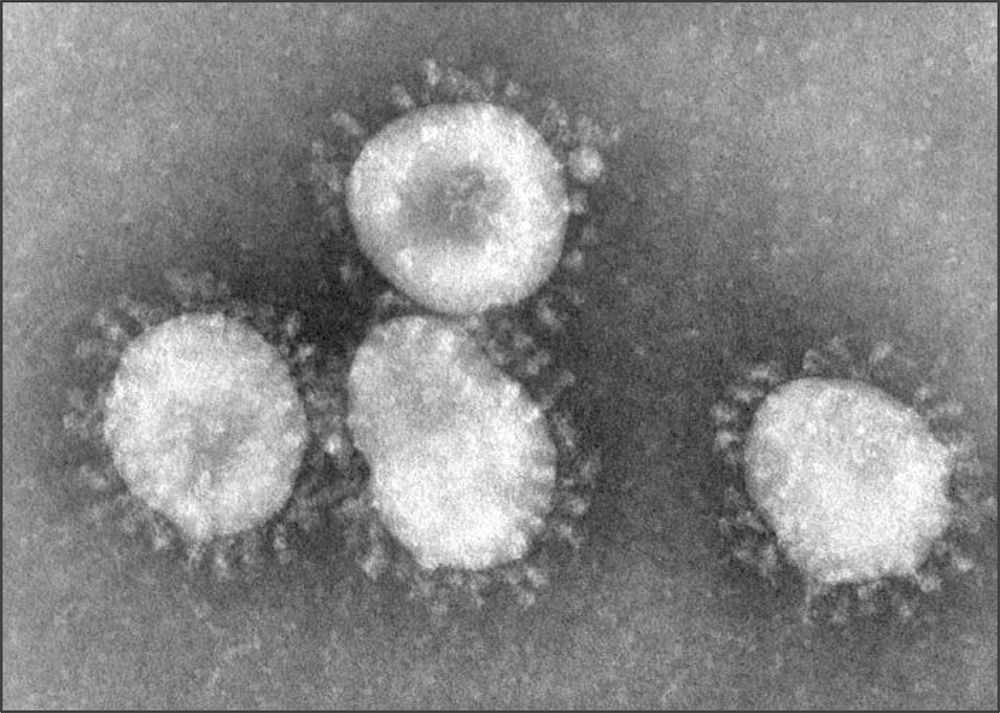
\includegraphics[width = 0.7\textwidth]{../images/coronavirus.png}
	\caption{Coronviruses as seen under a microscope. The fuzzy blobs on the cell surface are spike proteins, which the virus uses to gain entry to host cells. Figure courtesy F. Murphy and S. Whitfield, CDC.}
	\label{fig:coronavirus}
\end{figure}

Under a microscope, the two viruses look identical, and they use the same mechanism to infect human cells, when the spike protein on the virus surface bonds to the ACE2 enzyme on a human cell's membrane. So why did SARS fizzle, but SARS-CoV-2, a disease that is on average less harmful and less deadly to individuals who contract it, transform into a pandemic? The most likely explanation for the ability of SARS-CoV-2 to spread across far more countries and remain a public health threat even in the face of lockdowns is that it spreads more easily; that is, it is more \textdef{infectious}{infectious}{FILL IN}.

Part of the reason for the rapid spread of SARS-CoV-2 is that it can be spread by individuals that are asymptomatic, a method of transmission that was never found for SARS-CoV. But we also wonder if we can find a molecular explanation for the increased infectiousness of SARS-CoV-2.

In this chapter, we will place ourselves in the shoes of early SARS-CoV-2 researchers studying the new virus in January 2020. The virus's \textdef{genome}{genome}{FILL IN} (the 30,000 nucleotide sequence making up its DNA) was published on January 10, and an annotation of this genome showing the position of the virus's genes is shown in \autoref{fig:SARSCoV2Annotation}. Upon sequence comparison, SARS-CoV-2 was found to be related to several coronaviruses isolated from bats and distantly related to SARS-CoV.

\begin{figure}[h]
	\centering
	\mySfFamily
	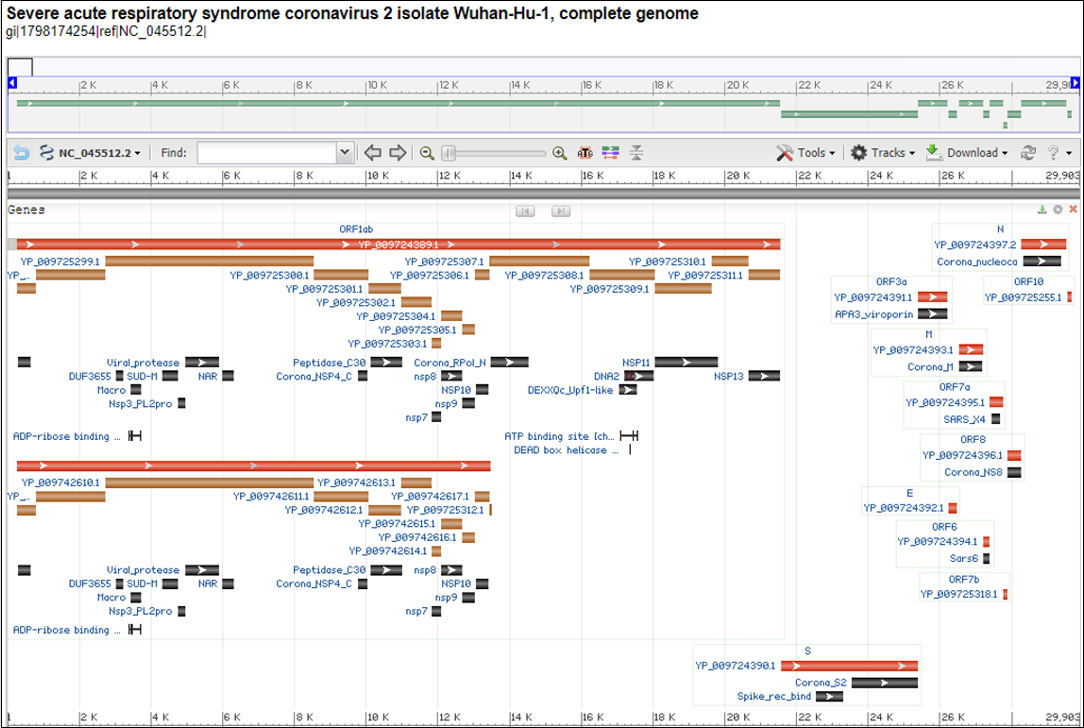
\includegraphics[width = 0.7\textwidth]{../images/SARSCoV2Annotation.png}
	\caption{An annotated genome of SARS-CoV-2. The Spike protein, found at the bottom of this image, is labeled "S" and begins at position 21,563. Accessed from GenBank: \url{https://go.usa.gov/xfzMM}}
	\label{fig:SARSCoV2Annotation}
\end{figure}

Recall from our discussion of transcription factors in \autoref{chapter:motifs} that by the central dogma of molecular biology, DNA is transcribed into RNA, which is then translated into protein. According to the genetic code, triplets of RNA nucleotides called codons are converted into single amino acids. The resulting chain of amino acids is called a \textdef{polypeptide}{polypeptide}{FILL IN}.

The polypeptide chain for the SARS-CoV-2 spike protein is shown below. Each of 20 possible amino acids is represented by a letter taken from the Latin alphabet (all letters except for "B", "J", "O", "U", "X", and "Z" are used for amino acids). Consider how such a global mayhem can ultimately be caused by something so tiny.

\texttt{>YP_009724390.1 S [organism=Severe acute respiratory syndrome coronavirus 2] [GeneID=43740568] \\
	MFVFLVLLPLVSSQCVNLTTRTQLPPAYTNSFTRGVYYPDKVFRSSVLHSTQDLFLPFFSNVTWFHAIHV
	SGTNGTKRFDNPVLPFNDGVYFASTEKSNIIRGWIFGTTLDSKTQSLLIVNNATNVVIKVCEFQFCNDPF
	LGVYYHKNNKSWMESEFRVYSSANNCTFEYVSQPFLMDLEGKQGNFKNLREFVFKNIDGYFKIYSKHTPI
	NLVRDLPQGFSALEPLVDLPIGINITRFQTLLALHRSYLTPGDSSSGWTAGAAAYYVGYLQPRTFLLKYN
	ENGTITDAVDCALDPLSETKCTLKSFTVEKGIYQTSNFRVQPTESIVRFPNITNLCPFGEVFNATRFASV
	YAWNRKRISNCVADYSVLYNSASFSTFKCYGVSPTKLNDLCFTNVYADSFVIRGDEVRQIAPGQTGKIAD
	YNYKLPDDFTGCVIAWNSNNLDSKVGGNYNYLYRLFRKSNLKPFERDISTEIYQAGSTPCNGVEGFNCYF
	PLQSYGFQPTNGVGYQPYRVVVLSFELLHAPATVCGPKKSTNLVKNKCVNFNFNGLTGTGVLTESNKKFL
	PFQQFGRDIADTTDAVRDPQTLEILDITPCSFGGVSVITPGTNTSNQVAVLYQDVNCTEVPVAIHADQLT
	PTWRVYSTGSNVFQTRAGCLIGAEHVNNSYECDIPIGAGICASYQTQTNSPRRARSVASQSIIAYTMSLG
	AENSVAYSNNSIAIPTNFTISVTTEILPVSMTKTSVDCTMYICGDSTECSNLLLQYGSFCTQLNRALTGI
	AVEQDKNTQEVFAQVKQIYKTPPIKDFGGFNFSQILPDPSKPSKRSFIEDLLFNKVTLADAGFIKQYGDC
	LGDIAARDLICAQKFNGLTVLPPLLTDEMIAQYTSALLAGTITSGWTFGAGAALQIPFAMQMAYRFNGIG
	VTQNVLYENQKLIANQFNSAIGKIQDSLSSTASALGKLQDVVNQNAQALNTLVKQLSSNFGAISSVLNDI
	LSRLDKVEAEVQIDRLITGRLQSLQTYVTQQLIRAAEIRASANLAATKMSECVLGQSKRVDFCGKGYHLM
	SFPQSAPHGVVFLHVTYVPAQEKNFTTAPAICHDGKAHFPREGVFVSNGTHWFVTQRNFYEPQIITTDNT
	FVSGNCDVVIGIVNNTVYDPLQPELDSFKEELDKYFKNHTSPDVDLGDISGINASVVNIQKEIDRLNEVA
	KNLNESLIDLQELGKYEQYIKWPWYIWLGFIAGLIAIVMVTIMLCCMTSCCSCLKGCCSCGSCCKFDEDD
	SEPVLKGVKLHYT}

We will ask ourselves two questions. First, can we use this sequence of amino acids to determine the structure of its spike protein? Second, once we know the structure of the SARS-CoV-2 spike protein, how does its structure and function differ from the same protein in SARS-CoV?

We will split our work on these questions over two parts. If you are already familiar with protein structure prediction, then you may want to skip ahead to the second part of the chapter, in which we discuss differences between the spike proteins of the two viruses.

\FloatBarrier
\phantomsection

\section{Protein Structure Prediction is Difficult}
\label{sec:structure_intro}
\phantomsection
\subsection{Determining protein structure is fundamental to understanding protein function}

In the \autoref{sec:introduction}, we showed the polypeptide chain for the SARS-CoV-2 spike protein. After this polypeptide chain is formed, it will "fold" into a three-dimensional shape and attach to the exterior of the virus. The folding process occurs spontaneously and without any outside influence, and the same polypeptide chain will almost always fold into the same 3-D structure in a manner of microseconds. This means that nature is applying some "magic algorithm" that produces the folded structure of a protein from its sequence of amino acids. But how does this algorithm work?

Predicting the folded structure of a polypeptide is called the \textdef{structure prediction problem}{structure prediction problem}{FILL IN}, and this problem is simple to state but deceptively difficult to solve. In fact, it has been an active area of biological research for several decades.

Why do we care about protein structure? Knowing a protein's structure is essential to determining its function and how it interacts with other proteins or molecules in its environment. Determining protein function is still an active area of research: there are still a few thousand proteins in humans alone whose function is unknown.

Furthermore,  a huge amount of biological research is devoted to understanding protein interactions. For example, a disease may be caused by a faulty protein, in which case researchers want to find a drug that binds to the protein and causes some change of interest in that protein, such as inhibiting its behavior.

For a more visual example of how protein structure affects protein function, consider the following video of a ribosome (which is a complex of RNA and proteins) translating a messenger RNA into protein. For translation to succeed, the ribosome needs to have a very precise shape, including a "slot" into which the messenger RNA strand can fit.

\texttt{NEED FIGURE HERE -- TO REPLACE VIDEO}\\
% include video id="TfYf_rPWUdY" provider="youtube" %

As we have seen throughout this course, molecular interactions are ruled by probability. Any two molecules may \textit{interact}, but their rate of \textit{dissociation} will be much higher if they do not fit together well. Furthermore, two colliding molecules need to have the correct orientation in order to produce an interaction

Because structure prediction is such a fundamental problem, researchers wish to catalog the varied shapes of different proteins. This variety is evident in \autoref{fig:different_protein_shapes_2020}, which shows the "proteins of the month" in 2020 named by the \textdef{Protein Data Bank (PDB)}{Protein Data Bank (PDB)}{FILL IN}. Yet the question remains: how do we know these protein structures?

\begin{figure}[h]
	\centering
	\mySfFamily
	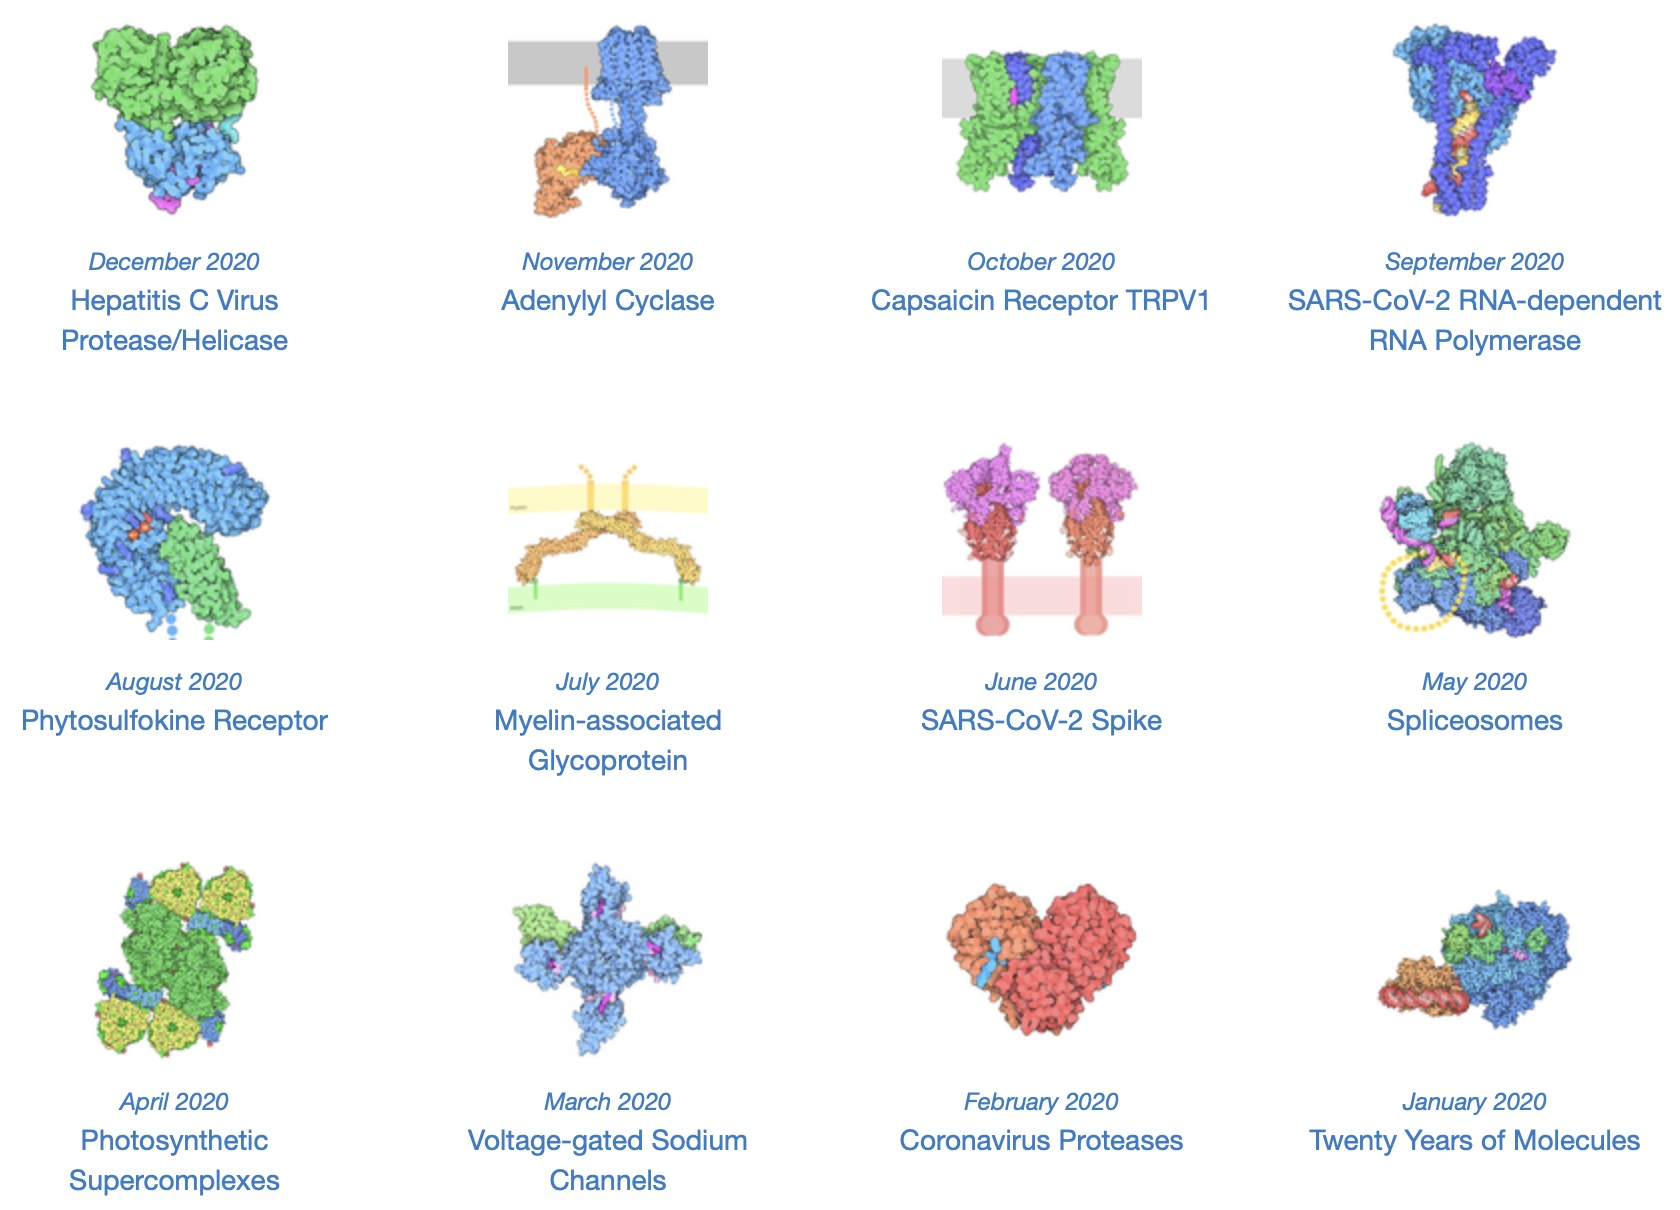
\includegraphics[width = 0.7\textwidth]{../images/different_protein_shapes_2020.jpg}
	\caption{Each "molecule of the month" in 2020 named by the PDB. These proteins have widely varying shapes and accomplish a wide variety of cellular tasks. Note that the SARS-CoV-2 spike protein was the molecule of the month in June 2020. Image courtesy: David Goodsell.}
	\label{fig:different_protein_shapes_2020}
\end{figure}

\FloatBarrier
\phantomsection
\subsection{Laboratory methods for determining protein structure}

We will introduce two popular and sophisticated laboratory methods for accurately determining protein structure. We appeal to high-quality videos explaining them if you are interested.

In \textdef{X-ray crystallography}{X-ray crystallography}{FILL IN}, researchers crystallize many copies of a protein and then shine an intense beam of X-rays at the crystal. The light hitting the protein is diffracted, creating patterns from which the position of every atom in the protein can be inferred. If you are interested in learning more about X-ray crystallography, check out the following excellent two-part video series from The Royal Institution.

\texttt{NEED FIGURE HERE -- TO REPLACE VIDEO}\\
% include video id="gLsC4wlrR2A" provider="youtube" %

\texttt{NEED FIGURE HERE -- TO REPLACE VIDEO}\\
% include video id="WJKvDUo3KRk" provider="youtube" %

X-ray crystallography is over a century old and has been the \textit{de facto} approach for protein structure determination for decades. Yet a newer method is now rapidly replacing X-ray crystallography.

In \textdef{cryo-electron microscopy (cryo-EM)}{cryo-electron microscopy (cryo-EM)}{FILL IN}, researchers preserve thousands of copies of a protein in non-crystalline ice and then examine these copies with an electron microscope. Check out the following YouTube video from the University of California San Francisco for a detailed discussion of cryo-EM.

\texttt{NEED FIGURE HERE -- TO REPLACE VIDEO}\\
% include video id="WJKvDUo3KRk" provider="youtube" %

Unfortunately, laboratory approaches for structure determination are expensive and cannot be used on all proteins. X-ray crystallography costs upward of \$2,000 per protein; furthermore, crystallizing a protein is a challenging task, and each copy of the protein must line up in the same way, which does not work for very flexible proteins. As for cryo-EM, an electron microscope costs upwards of millions of dollars. And to study bacterial proteins, we need to culture the bacteria in the lab, but microbiologists have estimated that less than 2\% of bacteria can currently be cultured.

Protein structures that have been determined experimentally are typically stored in the PDB. This database contains over 160,000 proteins, most of which have been added this century.

This number may seem large, but a recent study estimated that humans have between 620,000 and 6.13 million protein isoforms (i.e., differently-shaped protein variants). If we hope to catalog the proteins of all living things, then our work on structure determination is just beginning.

\FloatBarrier
\phantomsection
\subsection{What makes protein structure prediction so difficult?}

Predicting protein structure from amino acid sequence is very challenging. On the one hand, small perturbations in the sequence of a protein can drastically change the protein's shape and even render it useless. On the other, different amino acids can have similar chemical properties, and so some mutations will hardly change the shape of the protein. As a result, two very different amino acid sequences can fold into proteins with similar structure and comparable function.

For example, \autoref{fig:SequenceStructureExample} compares the sequences and structures of hemoglobin subunit alpha taken from three species: humans (PDB: 1si4), shortfin mako sharks (PDB: 3mkb), and emus (PDB: 3wtg). Hemoglobin is the oxygen-transport protein in the blood, consisting of two alpha "subunit" proteins and two beta subunit proteins that combine into a protein complex; because hemoglobin is well-studied and much shorter than the SARS-CoV-2 spike protein, we will use it as an example throughout this chapter. The alpha subunits for the three species are markedly different in terms of amino acid sequence, and yet their 3-D structures are essentially identical.

\begin{figure}[h]
	\centering
	\mySfFamily
	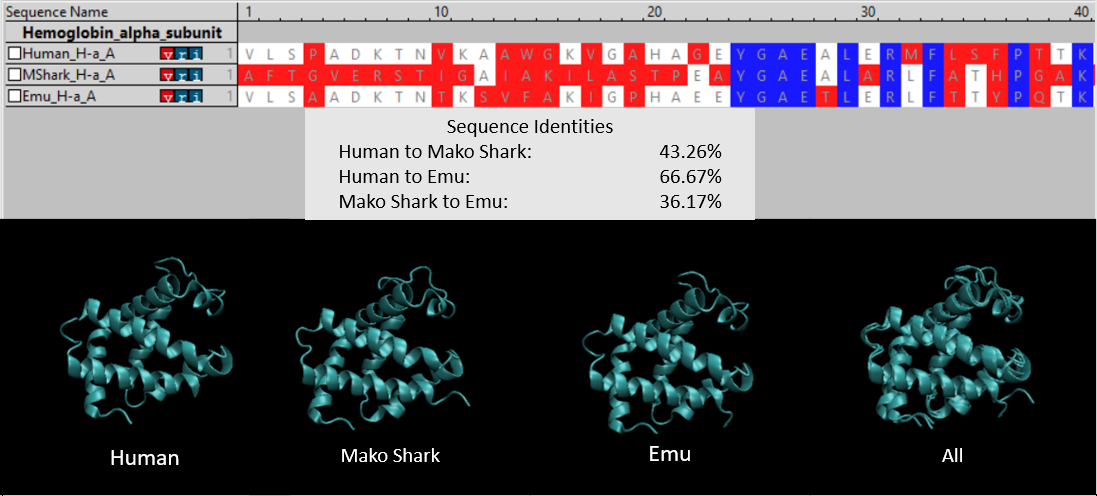
\includegraphics[width = 0.7\textwidth]{../images/SequenceStructureExample.png}
	\caption{(Top) An amino acid sequence comparison of the first 40 (out of 140) amino acids of hemoglobin subunit alpha for three species: human, shortfin mako shark, and emu. A column is colored blue if all three species have the same amino acid, white if two species have the same amino acid, and red if all amino acids are different. Sequence identity calculates the number of positions in two amino acid sequences that share the same amino acid. (Bottom) Side by side comparisons of the 3-D structures of the three proteins. The final figure on the right superimposes the first three structures to highlight their similarities.}
	\label{fig:SequenceStructureExample}
\end{figure}

Another reason why protein structure prediction is so difficult is because a polypeptide is very flexible, with the ability to rotate in multiple ways at each amino acid, which means that the polypeptide is able to fold into a staggering number of different shapes. A good analogy for polypeptide flexibility is the "Rubik's Twist" puzzle, shown in the video below, which consists of a linear chain of flexible blocks that can form a huge number of different shapes.

\texttt{NEED FIGURE HERE -- TO REPLACE VIDEO}\\
% include video id="auNLb75QRfg" provider="youtube" %

The flexibility of a polypeptide owes to the molecular structure of amino acids. As shown in \autoref{fig:AminoAcid}, an amino acid comprises four parts. In the center, a carbon atom (called the \textdef{alpha carbon}{alpha carbon}{FILL IN}) is connected to four different molecules: a hydrogen atom (H), a \textdef{carboxyl group}{carboxyl group}{FILL IN} (–COOH), an \textdef{amino group}{amino group}{FILL IN} (-NH\textsubscript{2}), and a \textdef{side chain}{side chain}{FILL IN} (denoted "R" and often called an \textdef{R group}{R group}{FILL IN}). The side chain is a molecule that differs between different amino acids and ranges in mass from a single hydrogen atom (glycine) up to -C\textsubscript{8}H\textsubscript{7}N (tryptophan).

\begin{figure}[h]
	\centering
	\mySfFamily
	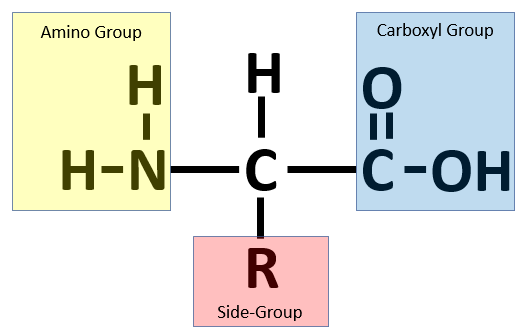
\includegraphics[width = 0.7\textwidth]{../images/AminoAcid.png}
	\caption{An amino acid consists of a central, alpha carbon attached to a hydrogen atom, a side group, a carboxyl group, and an amino group.}
	\label{fig:AminoAcid}
\end{figure}

To form a polypeptide chain, consecutive amino acids are linked together during a condensation reaction in which the amino group of one amino acid is joined to the carboxyl group of another, while a water molecule (H\textsubscript{2}O) is expelled (see in \autoref{fig:dipeptide_reaction}).

\begin{figure}[h]
	\centering
	\mySfFamily
	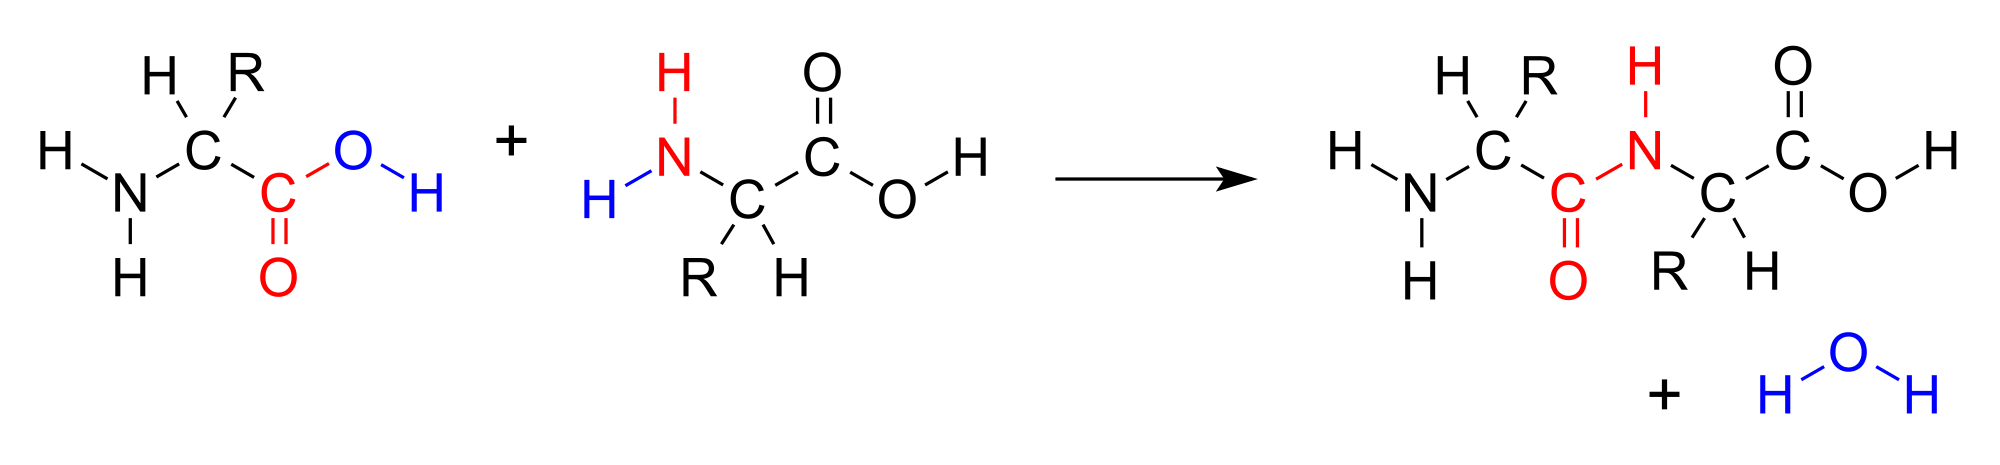
\includegraphics[width = 0.7\textwidth]{../images/dipeptide_reaction.png}
	\caption{A condensation reaction joins two amino acids into a "dipeptide" by joining the amino group of one amino acid to the carboxyl group of the other. A water molecule is expelled, which is why the reaction is a condensation reaction. Source: \url{https://bit.ly/3q0Ph8V}}
	\label{fig:dipeptide_reaction}
\end{figure}

The resulting bond that is produced between the carbon atom of one amino acid's carboxyl group and the nitrogen atom of the next amino acid's amino group, called a \textdef{peptide bond}{peptide bond}{FILL IN}, is very strong. The peptide has very little rotation around this bond, which is almost always locked at 180\textdegree. As peptide bonds are formed between adjacent amino acids, the polypeptide chain takes shape, as shown in \autoref{fig:backbone}.

\begin{figure}[h]
	\centering
	\mySfFamily
	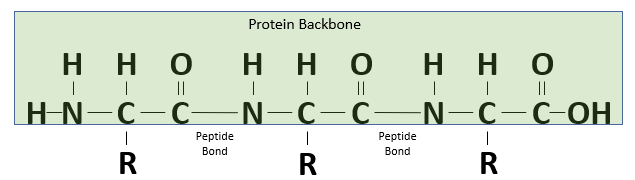
\includegraphics[width = 0.7\textwidth]{../images/Backbone.png}
	\caption{A protein backbone formed of three amino acids.}
	\label{fig:backbone}
\end{figure}

However, the bonds \textit{within} an amino acid, joining the alpha carbon to its carboxyl group and amino group, are not as rigid, and the polypeptide is free to rotate around these two bonds. This rotation produces two angles of interest, called the \textdef{phi angle (φ)}{phi angle (φ)}{FILL IN} and \textdef{phi angle (ψ)}{psi angle (ψ)}{FILL IN} (see \autoref{fig:torsion_angles}), which are formed at the alpha carbon's connections to its amino group and carboxyl group, respectively.

\begin{figure}[h]
	\centering
	\mySfFamily
	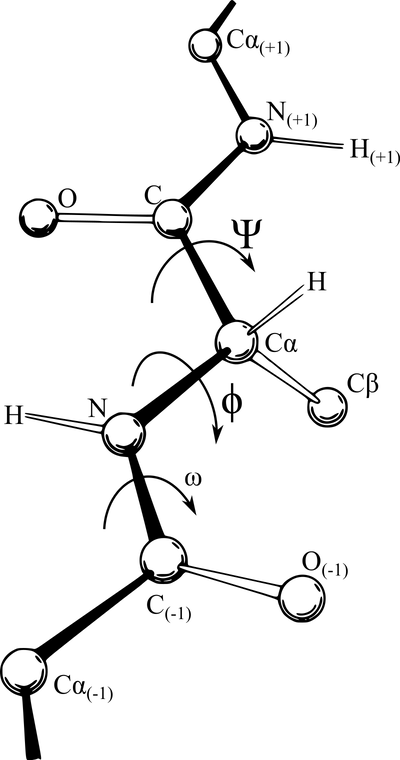
\includegraphics[width = 0.7\textwidth]{../images/torsion_angles.png}
	\caption{A polypeptide chain of multiple amino acids with the torsion angles φ and ψ indicated. The angle ω indicates the angle of the peptide bond, which is typically 180\textdegree. Image courtesy: Adam Rędzikowski.}
	\label{fig:torsion_angles}
\end{figure}

\url{https://youtu.be/1usemtIYe_s} is an excellent video from Jacob Elmer illustrating how changing φ and ψ at a single amino acid can drastically reorient a protein's shape.

A polypeptide with $$n$$ amino acids will have $$n - 1$$ peptide bonds, meaning that its shape is influenced by $$n - 1$$ phi angles and $$99 n - 1$$ psi angles. If each bond has $$k$$ stable conformations, then there are $$k^{2n-2}$$ total possible conformations of the polypeptide. For example, if $$k$$ is 3 and $$n$$ is just 100 (a short polypeptide), then the number of potential protein structures is more than the number of atoms in the universe! (The concept of combinatorial explosion, introduced in \autoref{chapter:chemotaxis}, appears again.) The ability for the protein to reliably find a single conformation using the magic algorithm despite such an enormous number of potential shapes is called \textdef{Levinthal's paradox}{Levinthal's paradox}{FILL IN}.

Although protein structure prediction is difficult, it is not impossible; nature's algorithm is not, after all, magic. Furthermore, researchers have spent decades cataloging the genomes of thousands of species. As a result, biologists know the \textit{sequence} of amino acids for many proteins whose structures have not been validated experimentally. In our case, although the SARS-CoV-2 genome was sequenced in January 2020, the structure of its spike protein was unknown at that time.  In the next section, we will place ourselves in the shoes of early SARS-CoV-2 researchers working before the structure of the virus's spike protein had been experimentally determined to see if we can predict its structure and give biologists a head start on fighting the pandemic.


\FloatBarrier
\phantomsection

\section{Ab initio Protein Structure Prediction}
\label{sec:ab_initio}
\phantomsection
\subsection{Distributing the work of protein structure prediction around the world}

The determination of the SARS-CoV-2 spike protein structure was remarkable because in many senses it was a community effort, dividing the computational heavy lifting over thousands of volunteers' computers around the world. Two leading structure prediction projects, Rosetta@home (\url{https://boinc.bakerlab.org}) and Folding@home (\url{https://foldingathome.org}), encourage volunteers to download their software and contribute to a gigantic \textit{distributed} effort to predict protein shape. Even with a modest laptop, a user can donate some of their computer's idle resources to contribute to the problem of protein structure prediction. But how does this software work?

Predicting a protein’s structure using only its amino acid sequence is called \textdef{\textit{ab initio} structure prediction}{\textit{ab initio} structure prediction}{FILL IN} (\textit{ab initio} means “from the beginning” in Latin). In this section, we will explain a little about how \textit{ab initio} structure prediction algorithms work.

As we dive into structure prediction, we should be more precise about two things. First, we will specify what we mean by the "structure" of a protein. Second, although we know that a polypeptide always folds into the same final three-dimensional shape, we have not said anything about \textit{why} a protein folds in a certain way. We will therefore need a better understanding of how the physicochemical properties of amino acids affect a protein's final structure.

\FloatBarrier
\phantomsection
\subsection{The four levels of protein structure}

Protein structure is a broad term that encapsulates four different levels of description. A protein's \textdef{primary structure}{primary structure}{FILL IN} refers to the amino acid sequence of the polypeptide chain. The primary structure of human hemoglobin subunit alpha can be downloaded as a FASTA file from the Protein Data Bank (\url{https://www.rcsb.org/structure/1SI4}), and the primary structure of the SARS-CoV-2 spike protein, which we showed earlier, can be downloaded from the Protein Data Bank (\url{https://www.rcsb.org/structure/6VXX}) as well.

A protein's \textdef{secondary structure}{secondary structure}{FILL IN} describes its highly regular, repeating intermediate substructures that form before the overall protein folding process completes. The two most common such substructures, shown in \autoref{hemoglobin_secondary_structure}, are \textdef{alpha helices}{alpha helices}{FILL IN and \textdef{beta sheets}{beta sheets}{FILL IN}. Alpha helices occur when nearby amino acids wrap around to form a tube structure; beta sheets occur when nearby amino acids line up side-by-side.

\begin{figure}[h]
	\centering
	\mySfFamily
	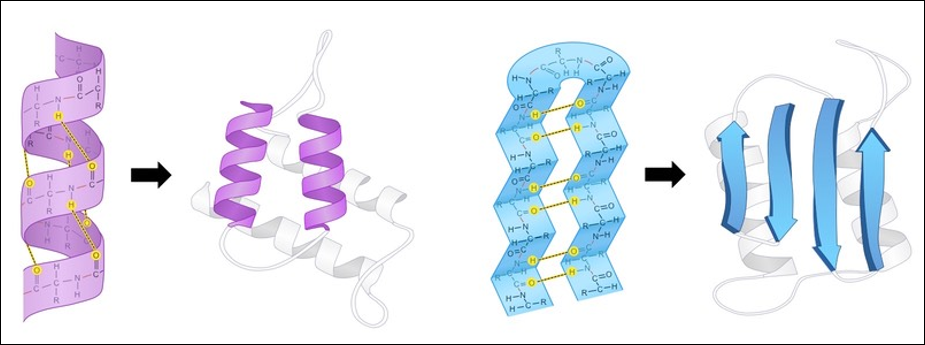
\includegraphics[width = 0.7\textwidth]{../images/hemoglobin_secondary_structure.png}
	\caption{General shape of secondary structure alpha helices (left) and beta sheets (right). Source: Cornell, B. (2016). https://ib.bioninja.com.au/higher-level/topic-7-nucleic-acids/73-translation/protein-structure.html}
	\label{fig:hemoglobin_secondary_structure}
\end{figure}

A protein's \textdef{tertiary structure}{tertiary structure}{FILL IN} describes its final 3D shape after the polypeptide chain has folded and is stable. Throughout this chapter, when discussing the "shape" or "structure" of a protein, we are almost exclusively referring to its tertiary structure. \autoref{fig:hemoglobin_tertiary_structure} shows the tertiary structure of human hemoglobin subunit alpha. For the sake of simplicity, \autoref{fig:hemoglobin_tertiary_structure} does not show the position of every atom in the protein but rather represents the protein shape as a composition of secondary structures.

\begin{figure}[h]
	\centering
	\mySfFamily
	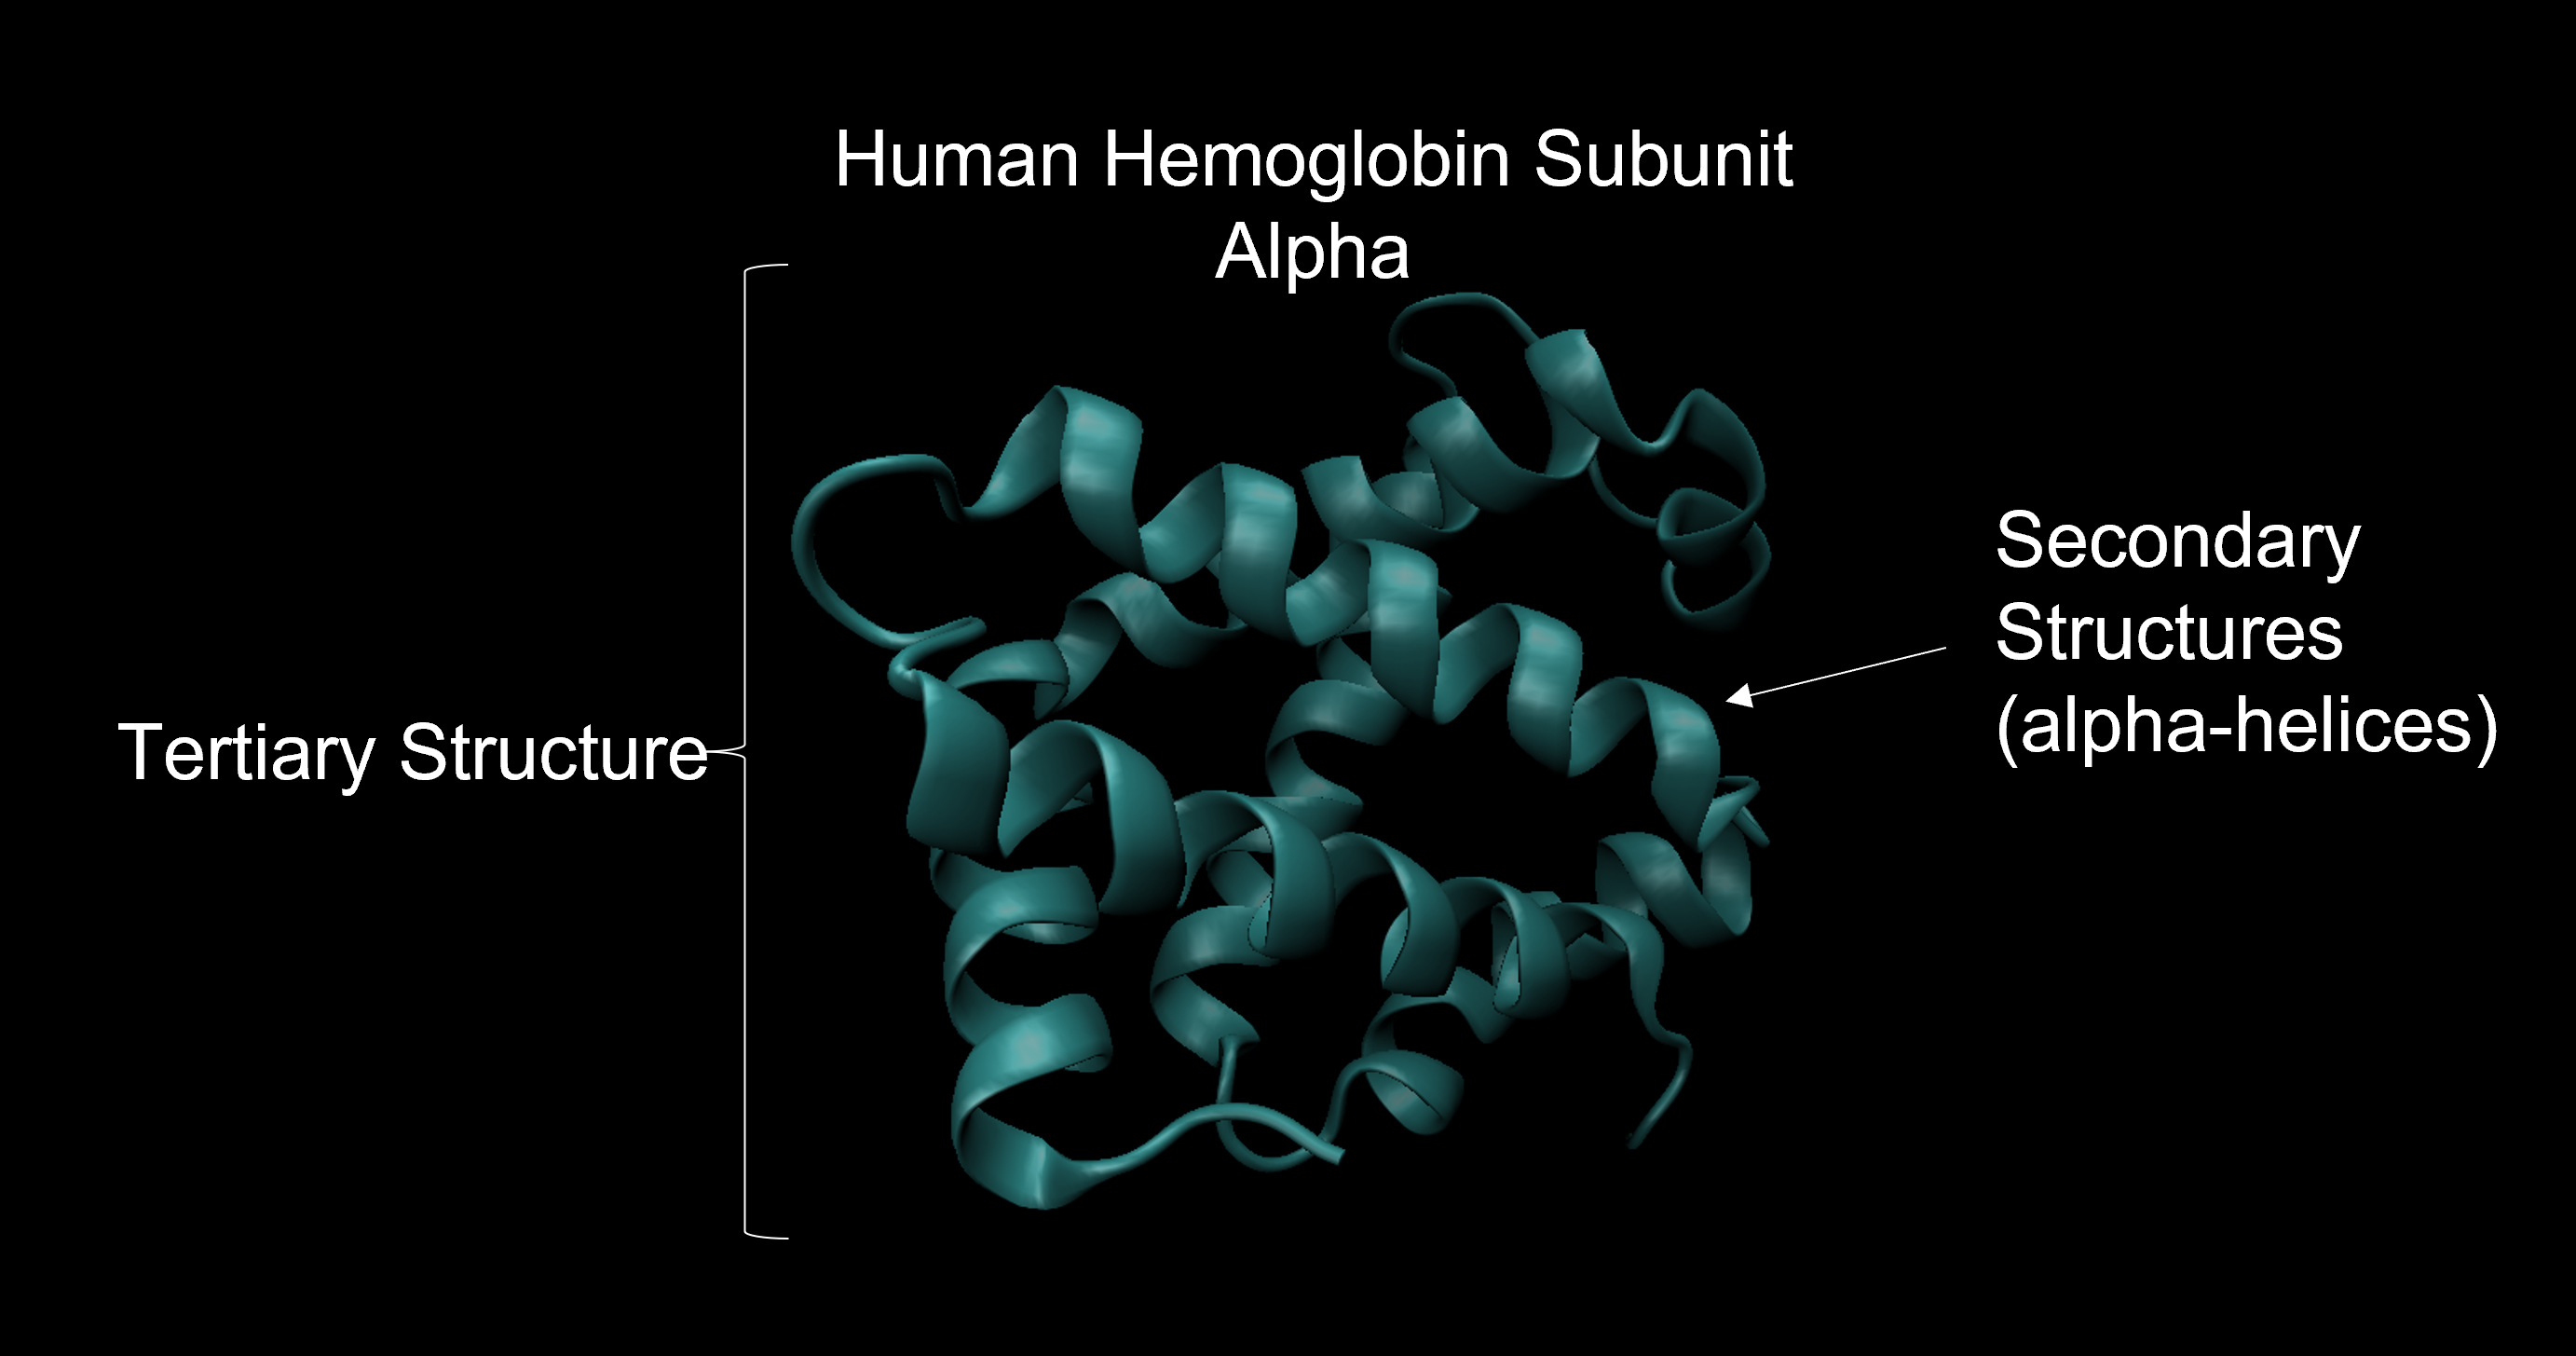
\includegraphics[width = 0.7\textwidth]{../images/hemoglobin_tertiary_structure.png}
	\caption{The tertiary structure of human hemoglobin subunit alpha. Within the structure are multiple alpha helix secondary structures. Source: https://www.rcsb.org/structure/1SI4}
	\label{fig:hemoglobin_tertiary_structure}
\end{figure}

Finally, some proteins have a \textdef{quaternary structure}{quaternary structure}{FILL IN}, which describes the protein’s interaction with other copies of itself to form a single functional unit, or a \textdef{multimer}{multimer}{FILL IN}. Many proteins do not have a quaternary structure and function as an independent monomer. The figure below shows the quaternary structure of hemoglobin, which is a multimer consisting of two alpha subunits and two beta subunits.

\begin{figure}[h]
	\centering
	\mySfFamily
	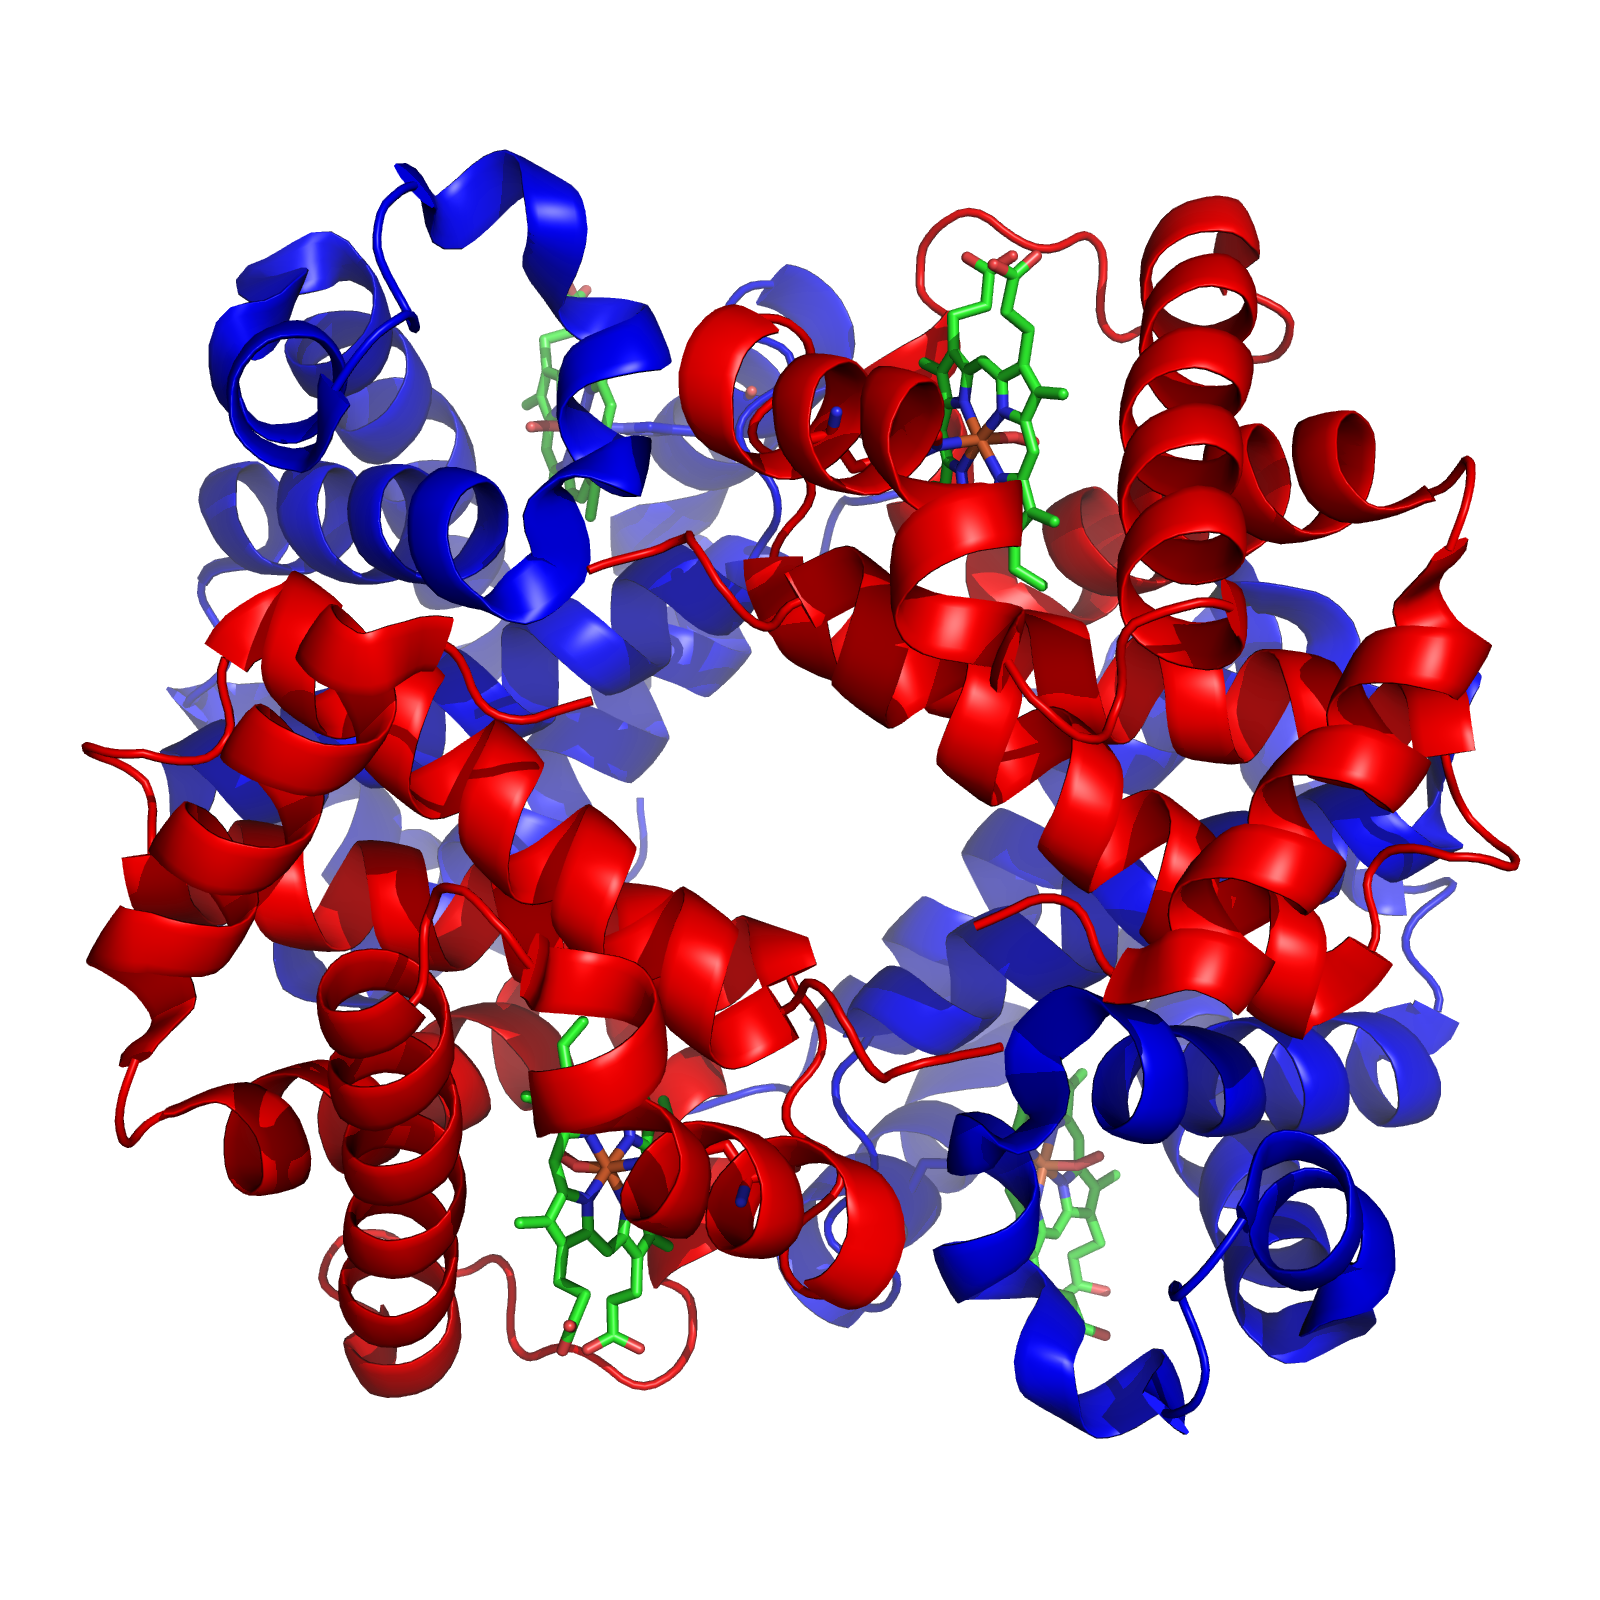
\includegraphics[width = 0.7\textwidth]{../images/hemoglobin_quaternary_structure.png}
	\caption{The quaternary structure of human hemoglobin, which consists of two alpha subunits (shown in red) and two beta subunits (shown in blue). Figure courtesy: Richard Wheeler}
	\label{fig:hemoglobin_quaternary_structure}
\end{figure}

As for SARS-CoV and SARS-CoV-2, the spike protein is a \textdef{homotrimer}{homotrimer}{FILL IN}, meaning that it is formed of three essentially identical units called \textdef{chains}{chains}{FILL IN}, each one translated from the corresponding region of the coronavirus's genome. When we talk about identifying the structure of the spike protein in this chapter, we typically are referring to the structure of a single chain.

The structural units making up proteins are often hierarchical, and the spike protein is no exception. Each spike protein chain is a \textdef{dimer}{dimer}{FILL IN}, consisting of two subunits called \textdef{S1}{S1}{FILL IN} and \textdef{S2}{S2}{FILL IN}. Each of these subunits further divides into \textdef{protein domains}{protein domains}{FILL IN}, distinct structural units within the protein that fold independently and are typically responsible for a specific interaction or function. For example, the SARS-CoV-2 spike protein has a \textdef{receptor binding domain (RBD)}{receptor binding domain (RBD)}{FILL IN} located on the S1 subunit of the spike protein that is responsible for interacting with the human ACE2 enzyme; the rest of the protein does not come into contact with ACE2. We will say more about the RBD soon.

\FloatBarrier
\phantomsection
\subsection{Proteins seek the lowest energy conformation}

Now that we know a bit more about how protein structure is defined, we will discuss why proteins fold in a certain way every time. In other words, what are the factors driving nature's magic protein folding algorithm?

Amino acids' variety of side chains causes the amino acids to have different chemical properties, which can lead to different conformations being more chemically "preferable" than others. For example, \autoref{fig:AminoAcidChart} shows the twenty standard amino acids occurring in proteins grouped by chemical properties. Nine of these amino acids are \textdef{hydrophobic}hydrophobic{}{FILL IN} (also called \textdef{non-polar}{non-polar}{FILL IN}), meaning that their side chains tend to be repelled by water, and as a result we tend to find these amino acids sheltered from the environment on the interior of the protein.

\begin{figure}[h]
	\centering
	\mySfFamily
	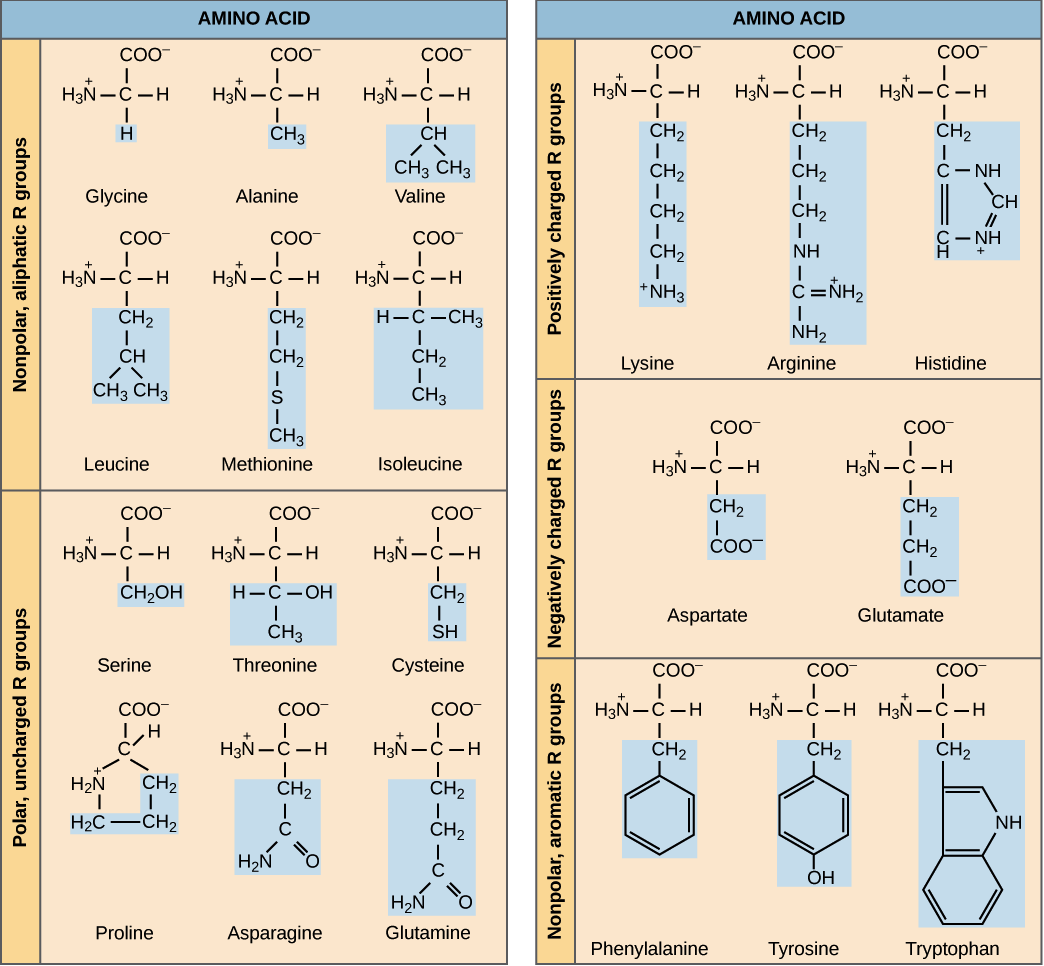
\includegraphics[width = 0.7\textwidth]{../images/AminoAcidChart.png}
	\caption{A chart of the twenty amino acid grouped by chemical properties. The side chain of each amino acid is highlighted in blue. Image courtesy: OpenStax Biology; https://openstax.org/books/biology/pages/1-introduction}
	\label{fig:AminoAcidChart}
\end{figure}

We can therefore view protein folding as finding the tertiary structure that is the most \textit{stable} given a polypeptide's primary structure. A central theme of the previous chapter on bacterial chemotaxis was that a system of chemical reactions moves toward equilibrium. The same principle is true of the magic folding algorithm; when a protein folds into its final structure, it is obtaining a conformation that is as chemically stable as possible.

To be more precise, the \textdef{potential energy}{potential energy}{FILL IN} (sometimes called \textdef{free energy}{free energy}{FILL IN}) of a molecule is the energy stored within an object due to its position, state, and arrangement. In molecular mechanics, the potential energy is made up of the sum of \textdef{bonded energy}{bonded energy}{FILL IN} and \textdef{non-bonded energy}{non-bonded energy}{FILL IN}.

Bonded energy derives from the protein's covalent bonds, as well as the angles of bonds between adjacent amino acids, and the torsion angles that we saw in the \autoref{sec:structure_intro}, as the protein bends and twists.

Non-bonded energy comprises \textdef{electrostatic interactions}{electrostatic interactions}{FILL IN} and \textdef{van der Waals interactions}{van der Waals interactions}{FILL IN}. Electrostatic interactions refer to the attraction and repulsion force from the electric charge between pairs of atoms. For example, some amino acids are \textdef{hydrophobic}{hydrophobic}{FILL IN}, meaning that they are repelled by water. If a folded protein structure were to have many hydrophobic amino acids on the outside of the protein, then these amino acids would be in constant contact with water molecules, which would repel them. Such a conformation would greatly increase the free energy of the molecule, as the nonpolar protein exterior would be forced inward.

As for van der Waals interactions, atoms are dynamic systems, with electrons constantly buzzing around the nucleus, as shown in \autoref{fig:van_der_waals_normal}.

\begin{figure}[h]
	\centering
	\mySfFamily
	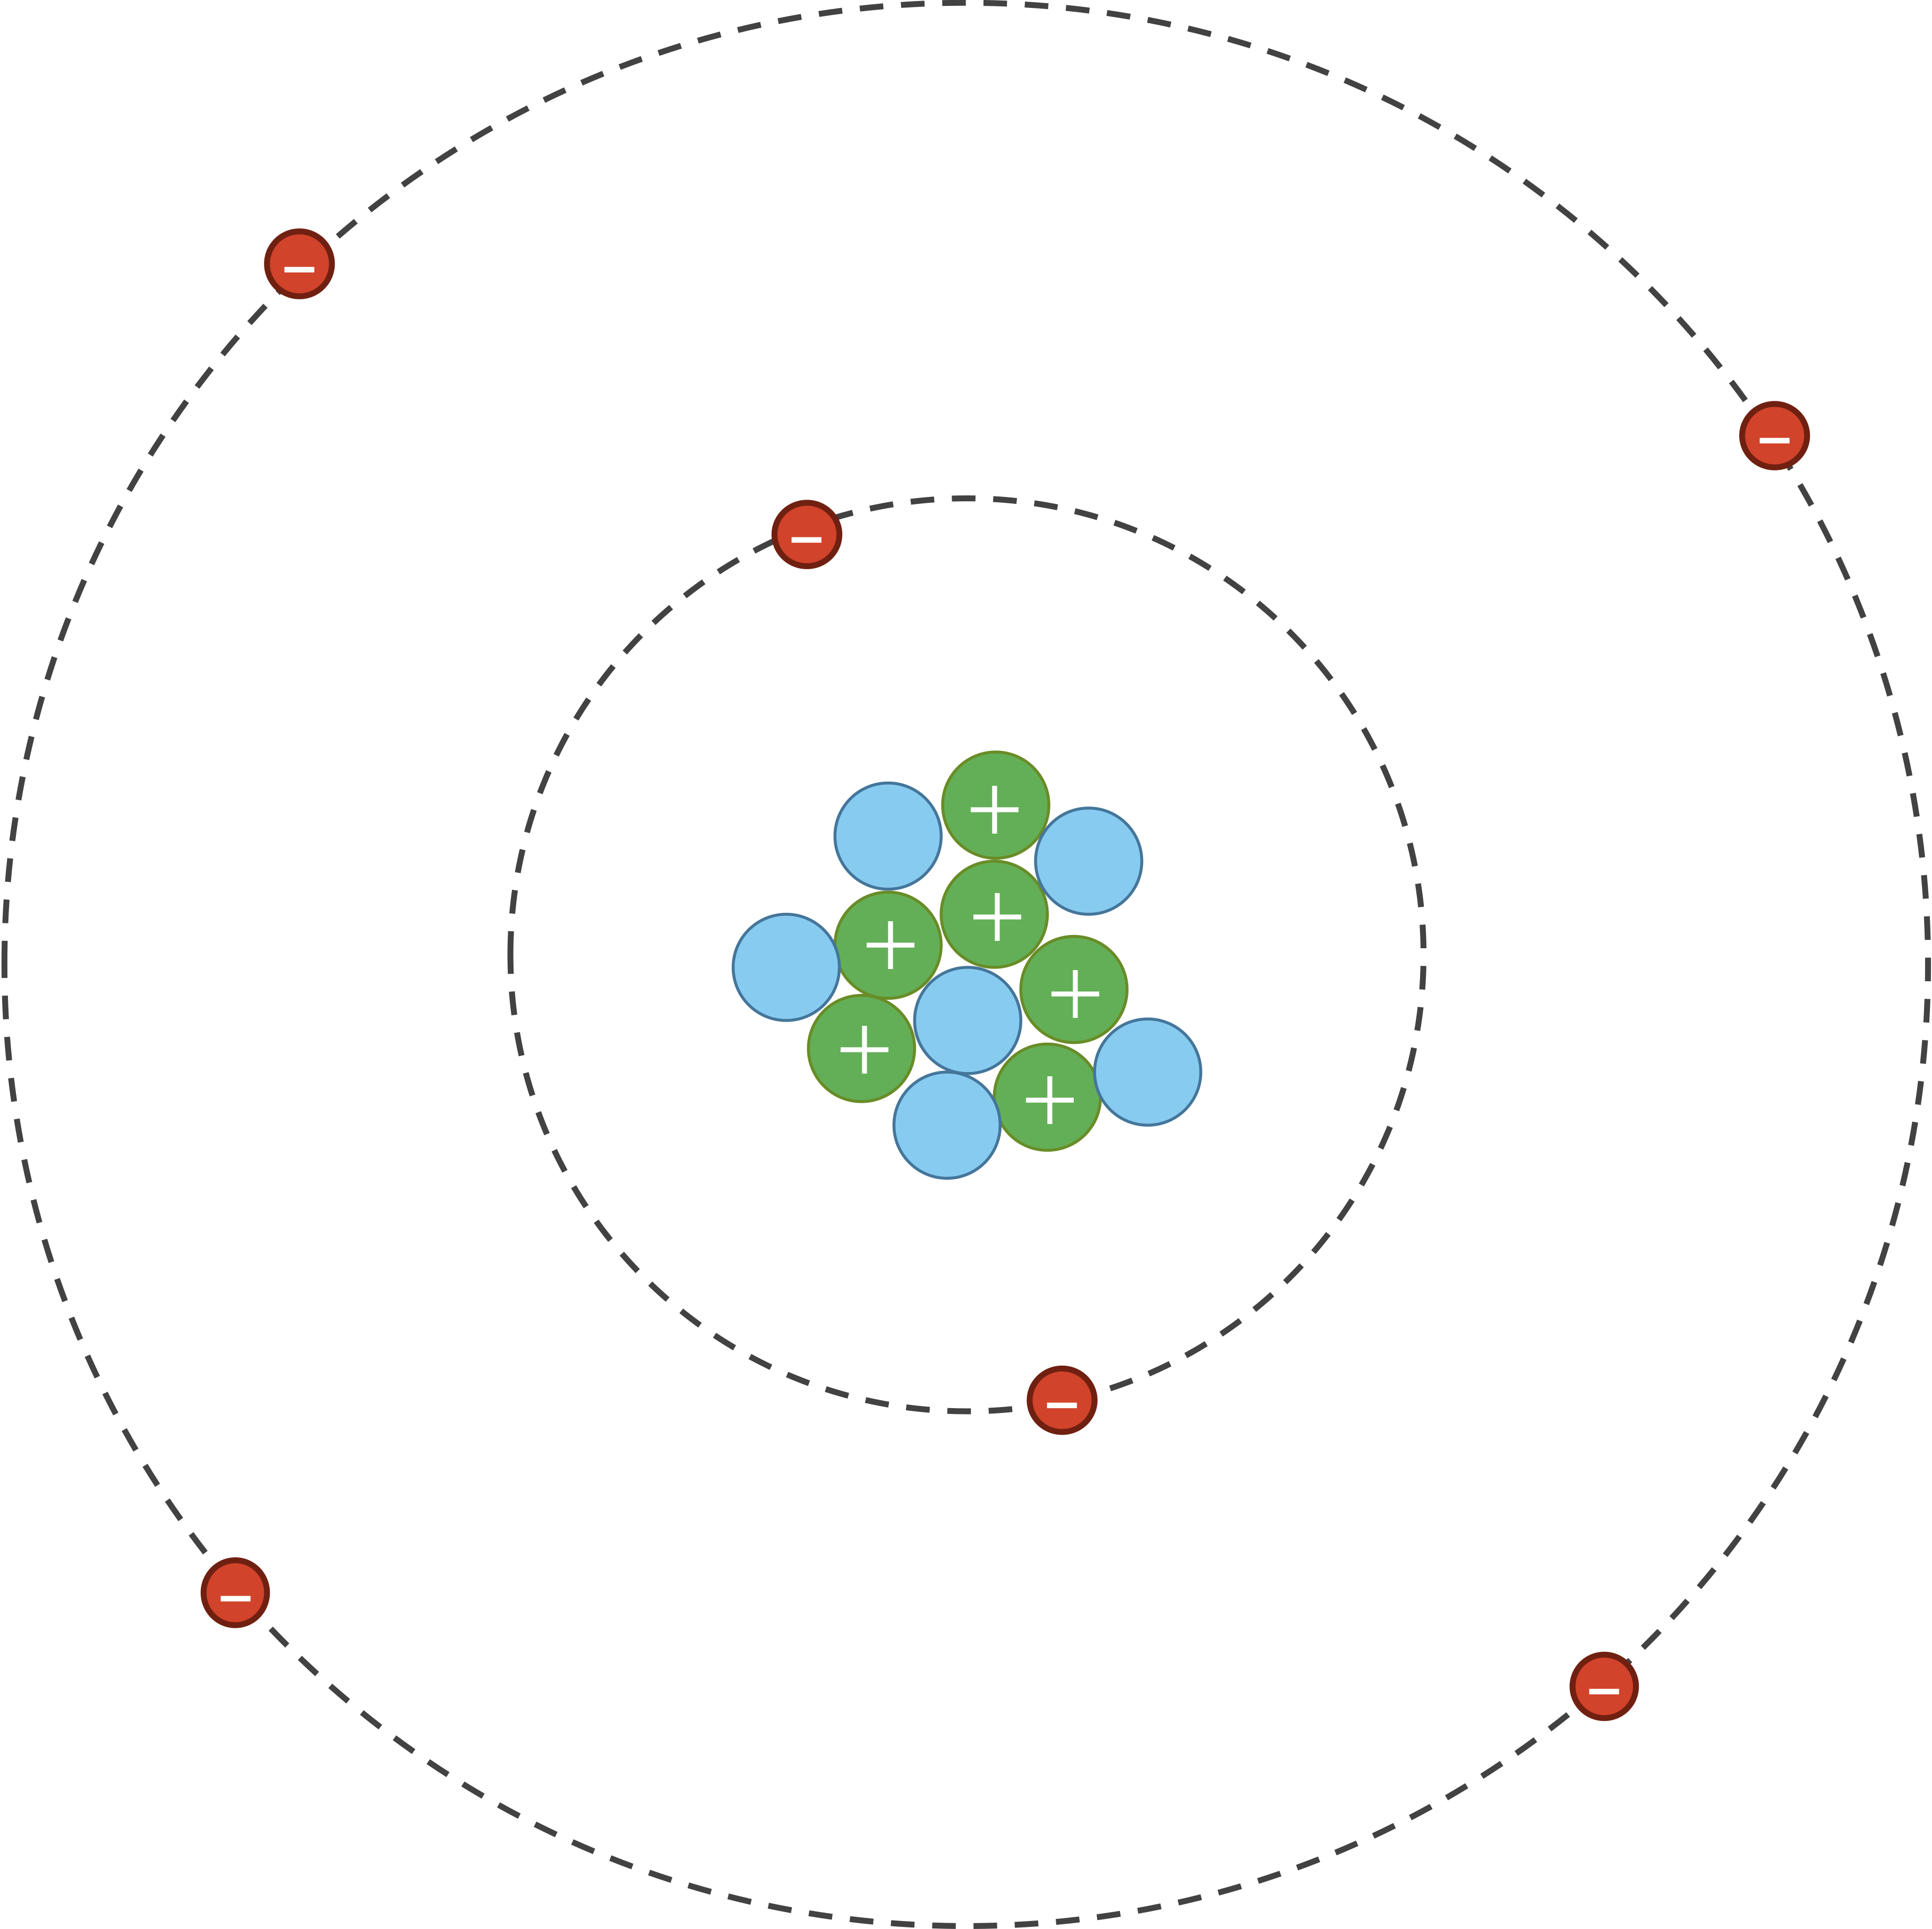
\includegraphics[width = 0.7\textwidth]{../images/van_der_waals_normal.png}
	\caption{A carbon-12 atom showing six positively charged protons (green), six neutrally charged neutrons (blue), and six negatively charged electrons (red). Under typical circumstances, the electrons will most likely be distributed uniformly around the nucleus.}
	\label{fig:van_der_waals_normal}
\end{figure}

However, due to random chance, the electrons in an atom could momentarily be unevenly distributed on one side of the nucleus. Because electrons are negatively charged, this uneven distribution will cause the atom to have a temporary negative charge on the side with the excess electrons and a temporary positive charge on the opposite side. As a result of this charge, one side of the atom may attract only the oppositely charged components of another atom, creating an \textdef{induced dipole}{induced dipole}{FILL IN} in that atom in turn as shown in \autoref{fig:van_der_waals}. Van der Waals forces refer to the attraction and repulsion between atoms because of induced dipoles.

\begin{figure}[h]
	\centering
	\mySfFamily
	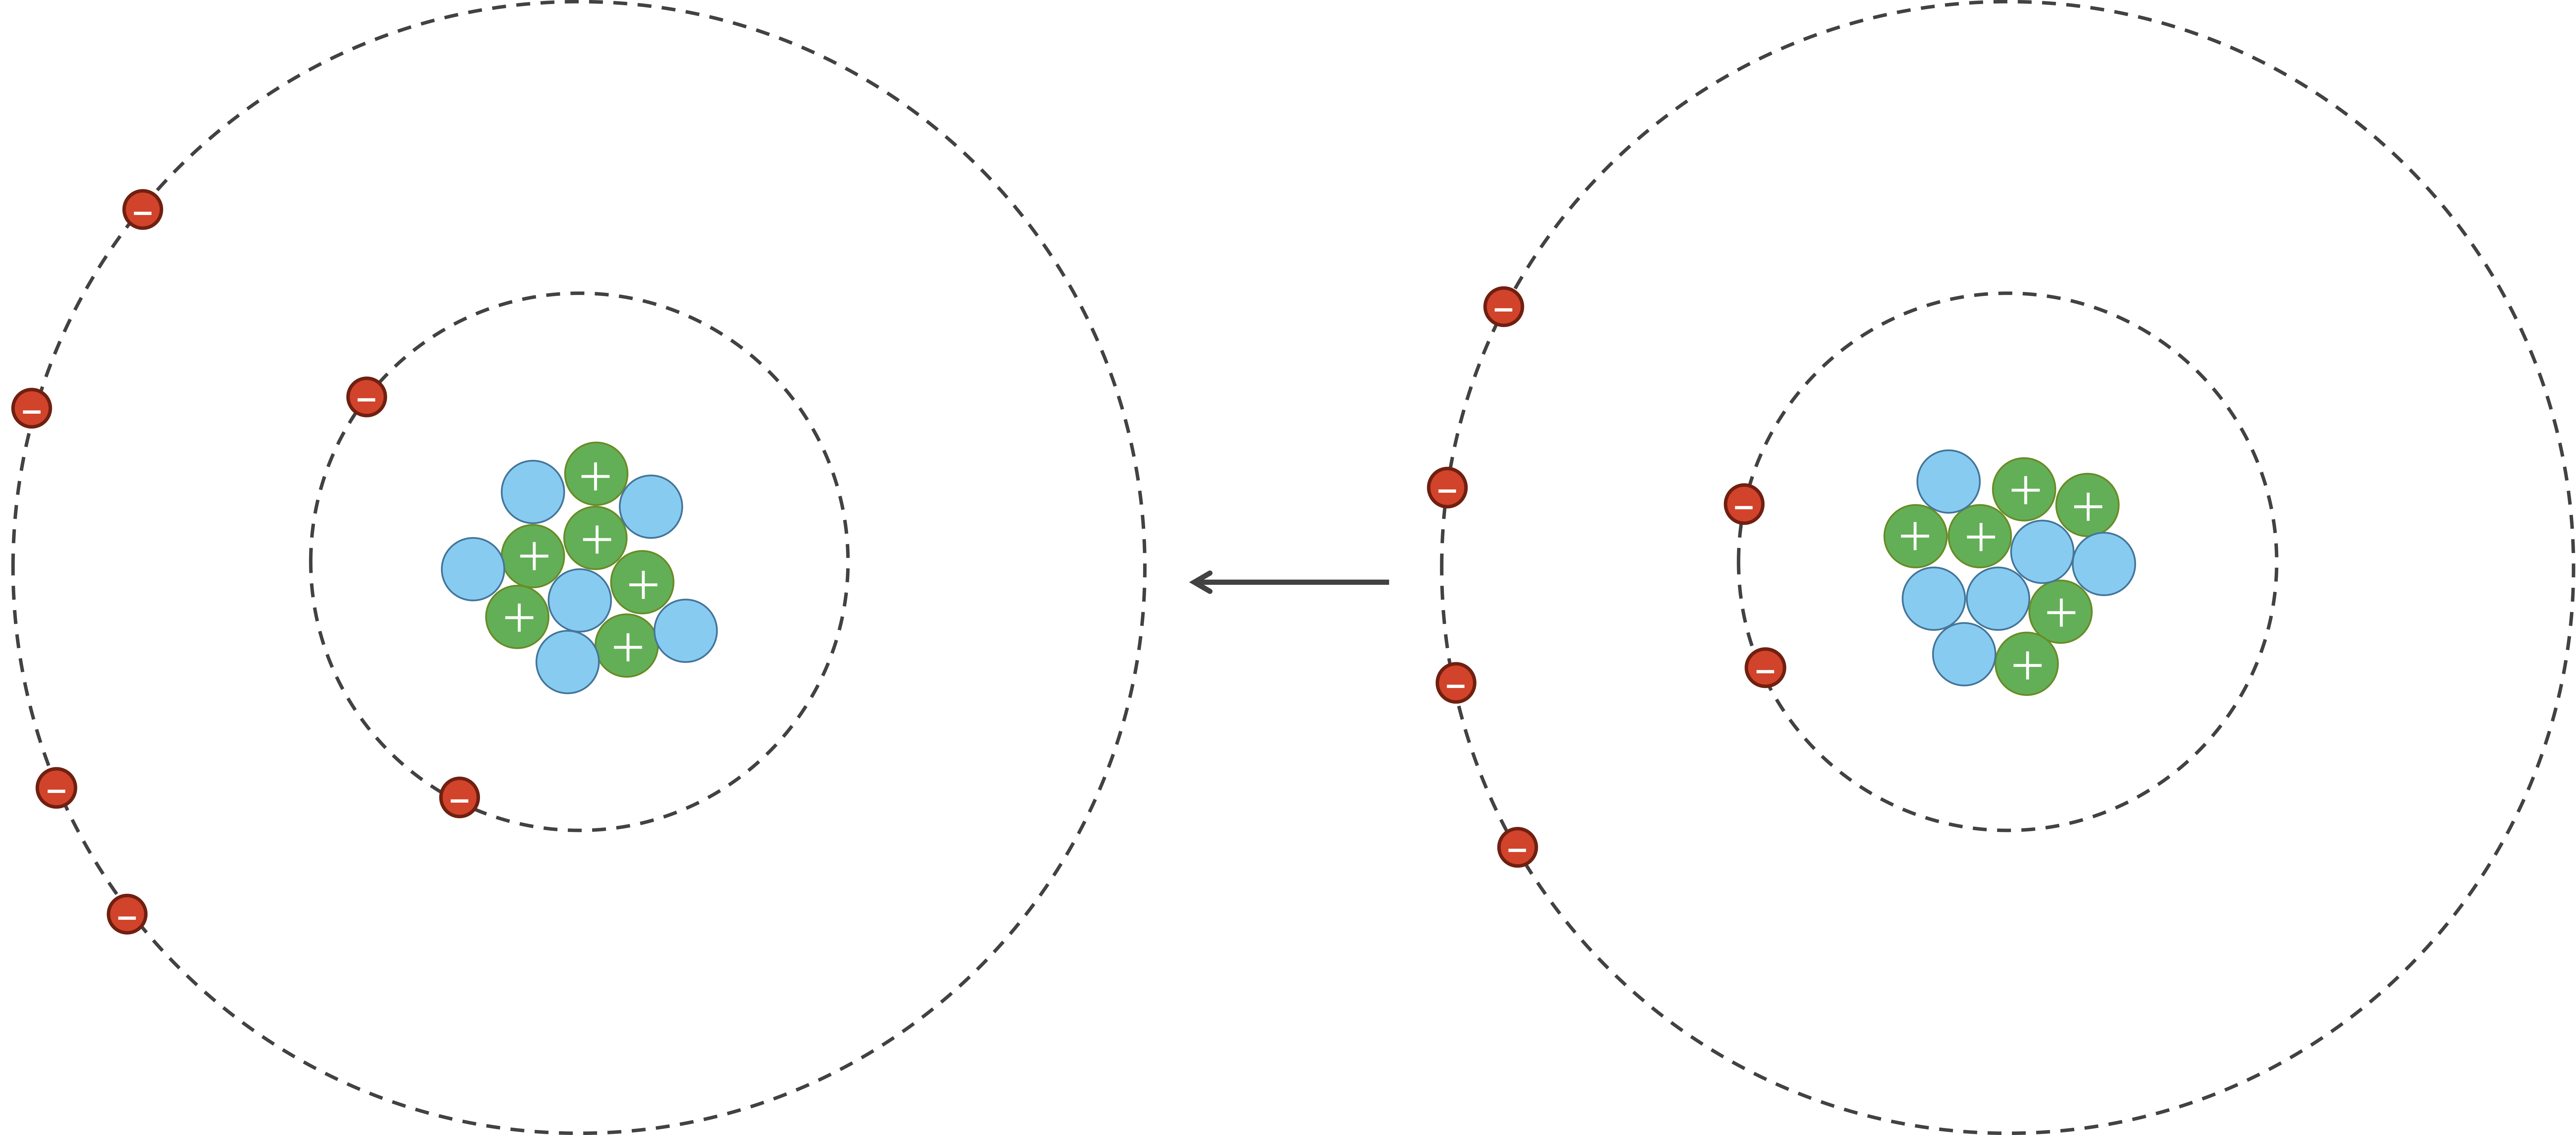
\includegraphics[width = 0.7\textwidth]{../images/van_der_waals.png}
	\caption{Due to random chance, the electrons in the atom on the left have clustered on the left side of the atom, creating a net negative charge on this side of the atom, and therefore a net positive charge on the right side of the atom. This polarity induces a dipole in the atom on the right, whose electrons are attracted because of van der Waals forces.}
	\label{fig:van_der_waals}
\end{figure}

As the protein folds, it seeks a conformation of \textit{lowest} total potential energy based on all these forces. For a simple analogy, imagine a ball on a slope, as shown in \autoref{fig:EnergyCartoon}. Even if the ball bounces around, it will tend to move down the slope. In this analogy, the lower points on the slope correspond to lower energy conformations of a polypeptide.

\begin{figure}[h]
	\centering
	\mySfFamily
	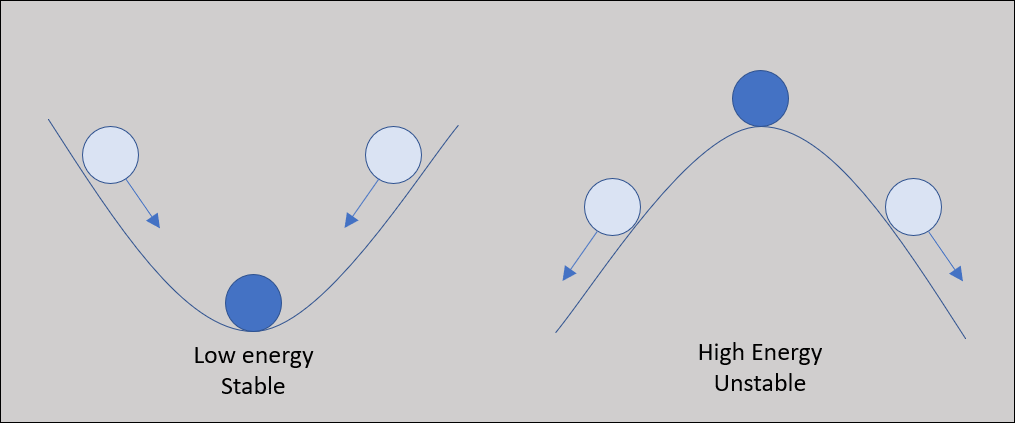
\includegraphics[width = 0.7\textwidth]{../images/EnergyCartoon.png}
	\caption{A ball on a hill offers a classic analogy for a protein folding into the lowest energy structure. As the ball is more likely to move down into a valley, a protein is more likely to fold into a low-energy conformation.}
	\label{fig:EnergyCartoon}
\end{figure}

\FloatBarrier
\phantomsection
\subsection{Modeling \textit{ab initio} structure prediction as an exploration problem}

Although a host of different algorithms have been developed for \textit{ab initio} protein structure through the years, these algorithms all find themselves solving a similar problem.

Biochemical research has contributed to the development of scoring functions called \textdef{force fields}{force fields}{FILL IN} that compute the potential energy of a candidate protein shape. As a result, for a given choice of force field, we can think of \textit{ab initio} structure prediction as solving the following problem: given a primary structure of a polypeptide, find its tertiary structure having minimum energy. This problem exemplifies an \textdef{optimization problem}{optimization problem}{FILL IN}, in which we look for an object maximizing or minimizing some function subject to constraints.

This formulation of protein structure may not strike you as similar to anything that we have done before in this course. However, consider once more a bacterium exploring an environment for food. Every point in the bacterium's "search space" is characterized by a concentration of attractant at that point, and the bacterium's goal is to reach the point of greatest attractant concentration.

In the case of structure prediction, our search space is the collection of all possible conformations of a given protein. And each point in this search space is characterized by the energy of the conformation at the point. Just as we imagined a ball rolling down a hill to find lower energy, we can now imagine "exploring" the space of all conformations of a polypeptide to find the conformation having lowest energy. This situation is illustrated in \autoref{fig:energy_landscape}, in which the height of each point represents the energy of the associated conformation; our goal, then, is to find the lowest point in this space.

\begin{figure}[h]
	\centering
	\mySfFamily
	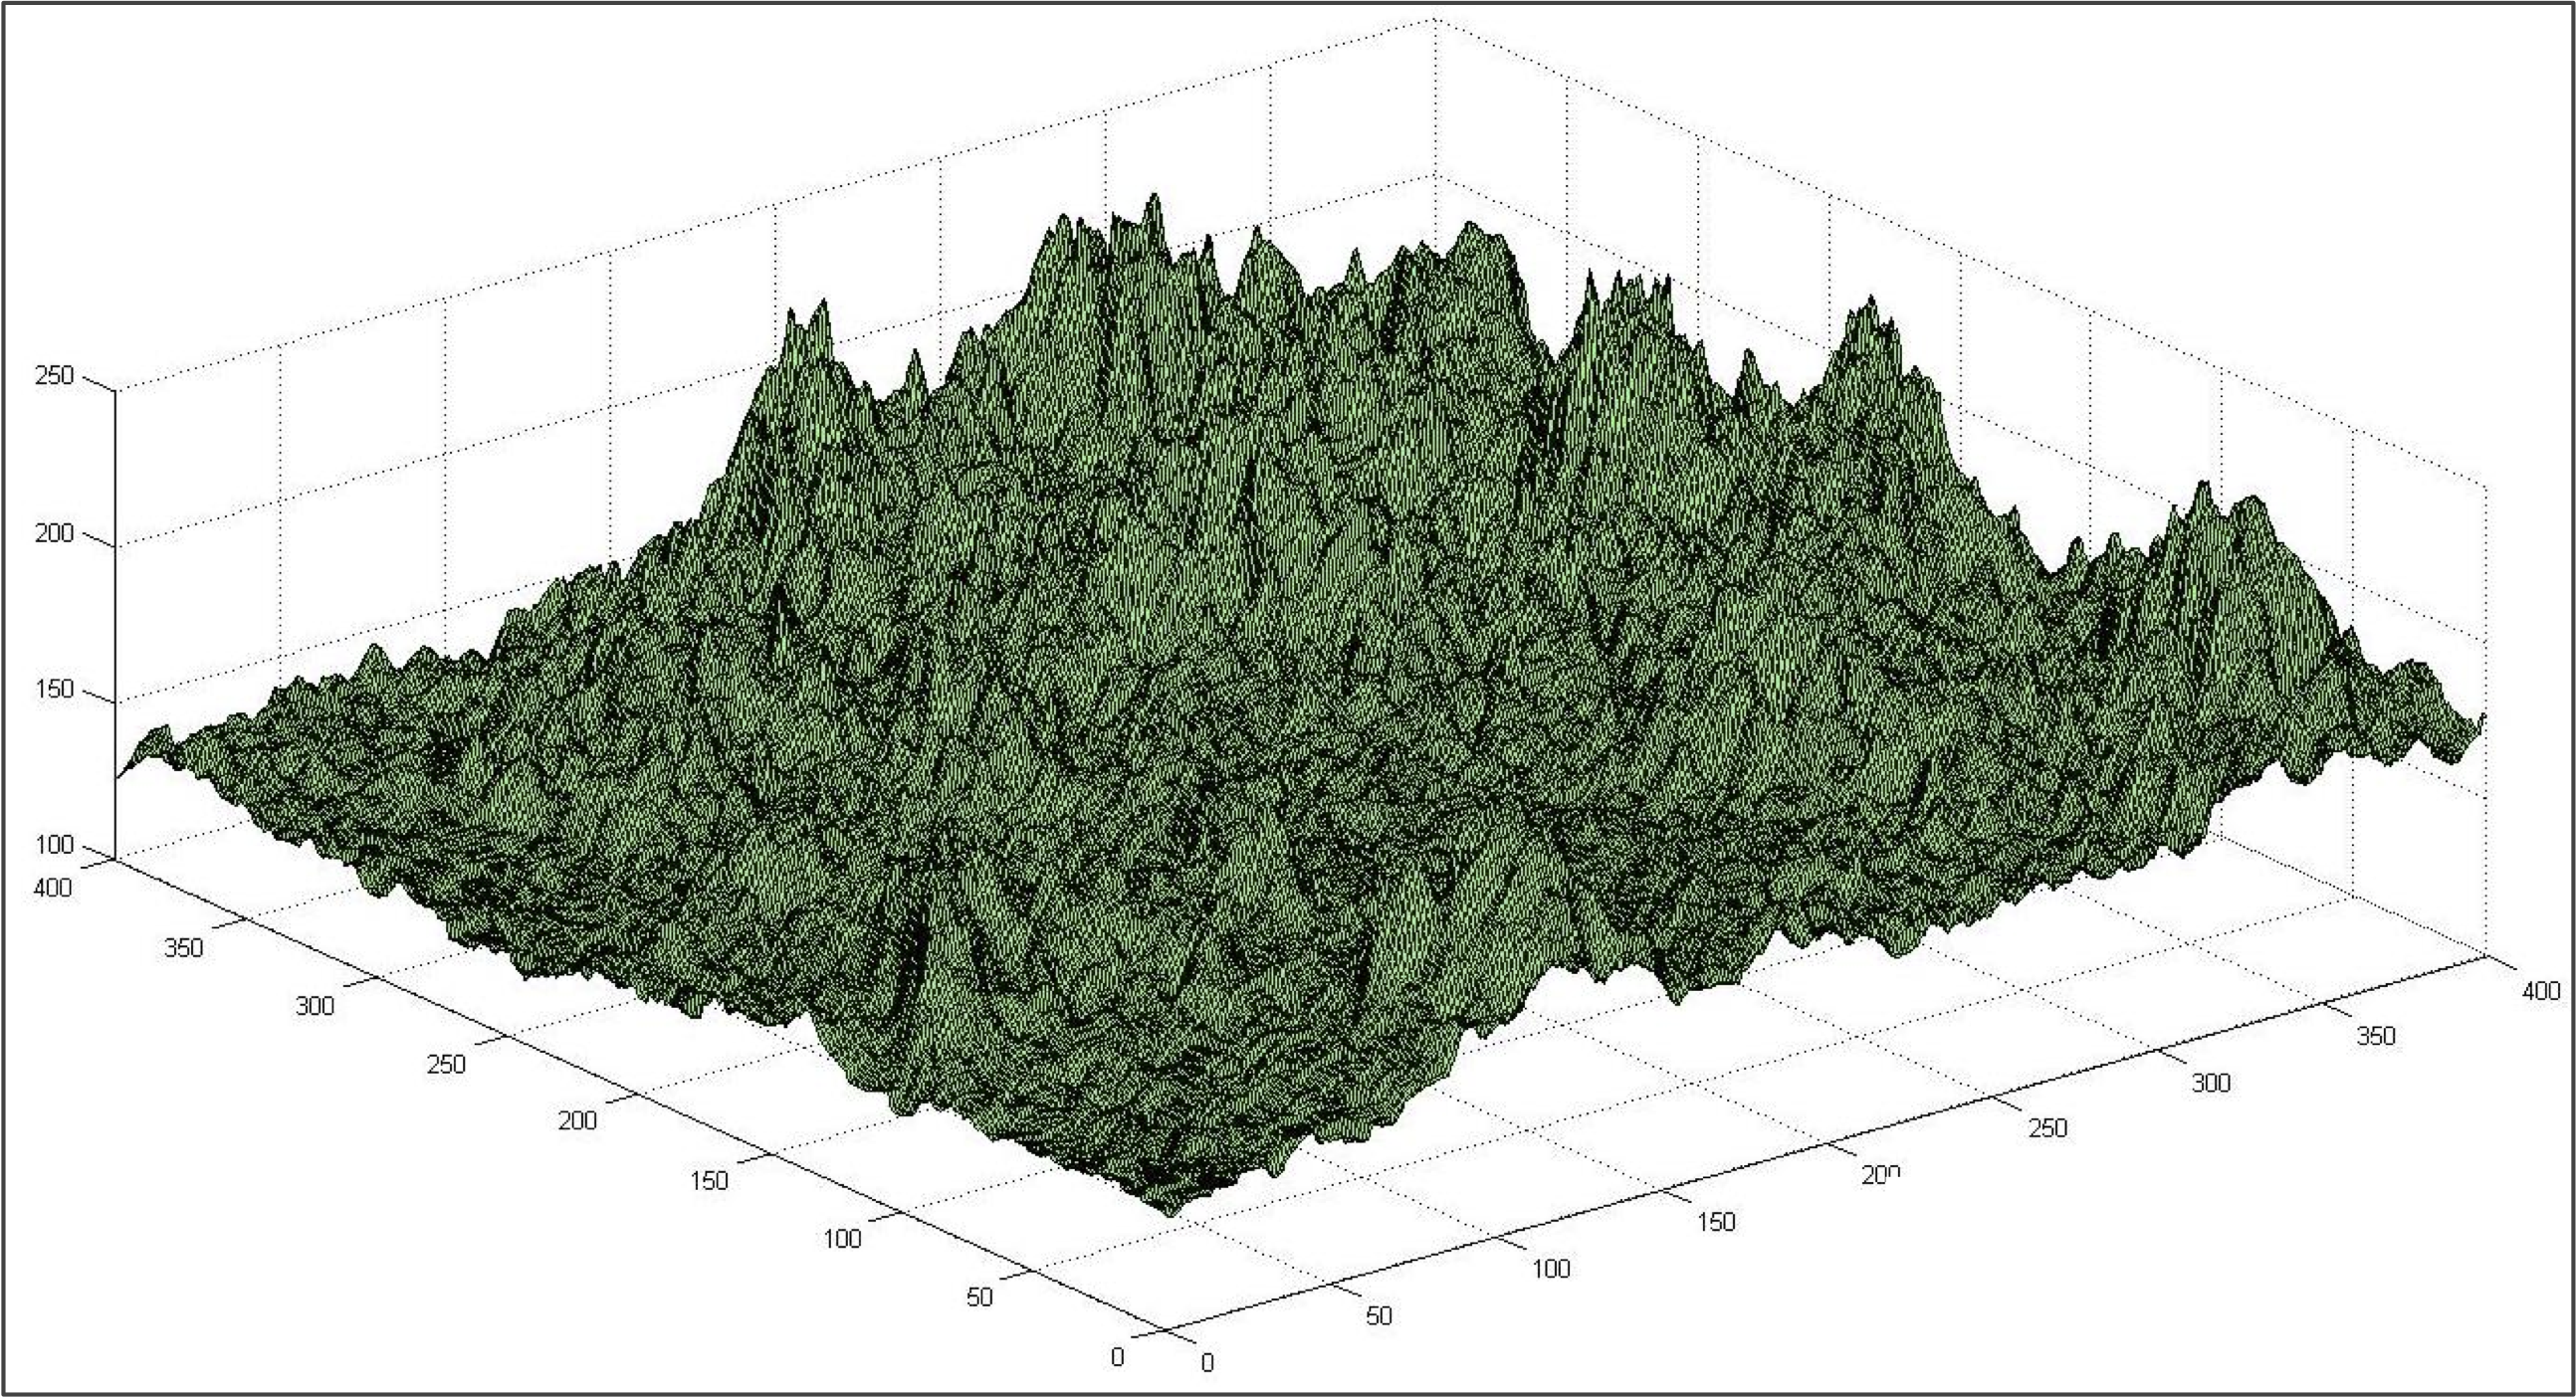
\includegraphics[width = 0.7\textwidth]{../images/energy_landscape.png}
	\caption{We can imagine each conformation of a given protein as occupying a point in a landscape, in which the elevation of a point corresponds to the energy of the conformation at that point. Image courtesy: David Beamish.}
	\label{fig:energy_landscape}
\end{figure}

\FloatBarrier
\phantomsection
\subsection{A local search algorithm for \textit{ab initio} structure prediction}

Now that we have conceptualized finding the most stable protein structure as exploring a search space, our next question is how to develop an algorithm to explore this space. Our idea is to adapt \textit{E. coli}'s clever exploration algorithm from \autoref:{chapter:chemotaxis) to our purposes. That is, at every step, we need to sense the "direction" in which the energy function decreases by the most, and then move in this direction.

Adapting this exploration algorithm to protein structure prediction requires us to develop a notion of what it means to consider the points "near" a given conformation in a protein search space. Many \textit{ab initio} algorithms will start at an arbitrary initial conformation and then make a variety of minor modifications to that structure (i.e., nearby points in the space), updating the current conformation to the modification that produces the greatest decrease in free energy. These algorithms then iterate the process of changing the protein structure to have greatest decrease in potential energy. We terminate our search when we reach a structure for which no changes to the structure reduce the free energy. Such an approach for structure prediction falls into a broad category of optimization algorithms called \textdef{local search algorithms}{local search algorithms}{FILL IN}.

Yet returning to the chemotaxis analogy, imagine what happens if we were to place many small sugar cubes and one large sugar cube into the bacterium's environment. The bacterium will sense the gradient not of the large sugar cube but of its \textit{nearest} attractant. Because the smaller food sources outnumber the larger food source, the bacterium will likely not reach the point of greatest attractant concentration. In terms of bacterial exploration, this is a feature, not a bug; if the bacterium exhausts one food source, then it will just move to another. But in terms of protein structure prediction, we should be worried of winding up in such a \textdef{local minimum}{local minimum}{FILL IN}, or a protein structure that does not have minimum free energy but does have  the property that no "neighboring" structures have lower energy.

\begin{qbox}[%
Do you see any ways in which we could improve our local search approach for structure prediction?
]\end{qbox}

Fortunately, we can modify our local search algorithm in a variety of ways. First, because the initial conformation has a huge influence on the final conformation, we could run the algorithm multiple times with different starting conformations. This is analogous to allowing multiple bacteria to explore their environment at different starting points.

Second, every time we reach a local minimum, we could allow ourselves to change the structure with some probability, thus giving our local search algorithm the chance to "bounce" out of the local minimum. In an approach called \textdef{simulated annealing}{simulated annealing}{FILL IN}, we start our local search with this probability high and reduce it over time, so that eventually we will settle into some local minimum that serves as our predicted structure. Once again, randomness helps us solve our problems!

\FloatBarrier
\phantomsection
\subsection{Applying an \textit{ab initio} algorithm to a protein sequence}

To run an \textit{ab initio} structure prediction algorithm on a real protein, we will use a software resource called QUARK (\url{https://zhanglab.ccmb.med.umich.edu/QUARK/}). QUARK is built upon the ideas discussed in the previous section, with some added features. For example, its algorithm applies a combination of \textit{multiple} scoring functions to look for the lowest energy conformation across all of these functions.

Despite the sophistication of software like QUARK, Levinthal's paradox means that the search space of all possible structures for a protein is so large that accurately predicting large protein structures with \textit{ab initio} modeling remains very difficult, and QUARK limits us to proteins with at most 200 amino acids. Since the SARS-CoV-2 spike protein contains 1281 amino acids, we will instead apply this software to the shorter human hemoglobin subunit alpha. \tutorial[https://biologicalmodeling.org/coronavirus/tutorial_ab_initio]

\FloatBarrier
\phantomsection
\subsection{Toward a faster approach for protein structure prediction}

\autoref{fig:ab_initio_results} the top five structures produced by QUARK for human hemoglobin subunit alpha, along with the protein's experimentally verified structure. It takes a keen eye to see any differences between these structures. We conclude that although \textit{ab initio} prediction is slow, it is still able to accurately reconstruct a model of this protein from its amino acid sequence.

\begin{figure}[h]
	\centering
	\mySfFamily
	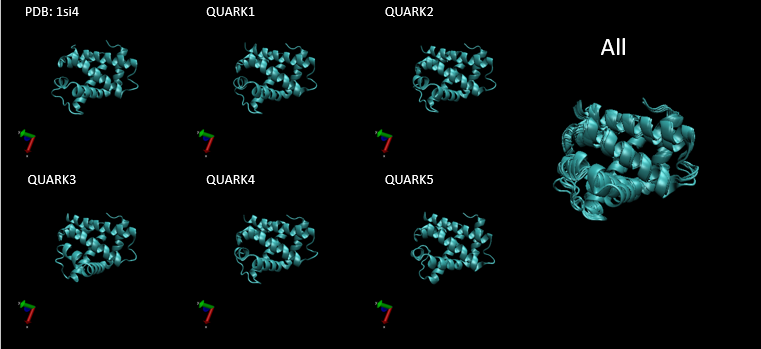
\includegraphics[width = 0.7\textwidth]{../images/ab_initio_results.png}
	\caption{A protein structure of human hemoglobin subunit alpha along with five \textit{ab initio} models of this protein produced by QUARK. We can see how close all five models are to the experimentally verified structure, as shown in the superimposition of all six structures at right.}
	\label{fig:ab_initio_results}
\end{figure}

Yet we also wonder whether we can speed up our structure prediction algorithms so that they will scale to a larger protein like the SARS-CoV-2 spike protein. In the next section, we will learn about another type of protein structure prediction that uses a database of known structures.

\begin{qbox}[%
What known protein structure(s) would you first want to consult when studying the SARS-CoV-2 spike protein?
]\end{qbox}

\FloatBarrier
\phantomsection

\section{Homology Modeling}
\label{sec:homology}
\phantomsection
\subsection{Homology modeling finds a similar protein structure}

In the \autoref{ab_initio}, we saw that \textit{ab initio} structure prediction of a long protein like the SARS-CoV-2 spike protein can be time consuming and error prone. As we mentioned in the \autoref{structure_intro}, however, researchers have entered over 160,000 experimentally verified structure entries into the PDB. With every new structure that we identify, we gain a little more insight into nature's magic protein folding algorithm. In \textdef{homology modeling}{homology modeling}{FILL IN} (also called \textdef{comparative modeling}{comparative modeling}{FILL IN}), we use the information contained in known structures to help us predict the structure of a protein with unknown structure.

The structure of the SARS-CoV spike protein was determined in 2003 and entered in the PDB. The amino acid \textit{sequence} of this \textdef{homologous protein}{homologous protein}{FILL IN} is 96\% similar to that of the SARS-CoV-2 spike protein. Assuming that the structure of the two spike proteins is similar, we will use SARS-CoV spike protein's known structure as a guide to help us predict the structure of the SARS-CoV-2 spike protein. In other words, if the search space of all conformations of the SARS-CoV-2 spike protein is enormous, why not restrict it to those structures that are similar to the SARS-CoV spike protein structure?

In the case of the SARS-CoV-2 spike protein, we already know that we want to use the SARS-CoV spike protein as a template. However, if we do not know which template to use before we begin, then we can use a search algorithm such as BLAST to find a protein with known structure that has similar sequence to our protein of interest.

\FloatBarrier
\phantomsection
\subsection{A similar structure reduces the size of the search space}

Once we have found a similar protein, we need to use it to help us predict the structure of our protein. One way of doing so is to include a "similarity term" that subtracts a structure's similarity to the template structure from the structure's total energy. That is, the more similar that a candidate structure is to the template, the more negative the contribution of this similarity term. To continue our search space analogy, the template protein "pulls down" the energy values of nearby structures.

Another way to perform homology modeling is to account for variance in similarity across different regions of the two proteins. For example, even though the SARS-CoV and SARS-CoV-2 genomes are 96\% similar, this does not mean that all of their proteins are 96\% similar. When we look at genomes from related species, we expect to see \textdef{conserved regions}{conserved regions}{FILL IN} where the species are very similar and other \textdef{variable regions}{variable regions}{FILL IN} where the species are more different than the average. For example, the spike proteins of SARS-CoV and SARS-CoV-2 are only 76\% similar.

The phenomenon of conserved and variable regions even occurs within individual genes. For example, \autoref{fig:} shows that within a spike protein subunit, the S2 domain is 90\% similar between the two viruses, whereas the S1 domain is only 64\% similar. Furthermore, there are nested subregions of greater or less variability within each of the two domains.

\begin{figure}[h]
	\centering
	\mySfFamily
	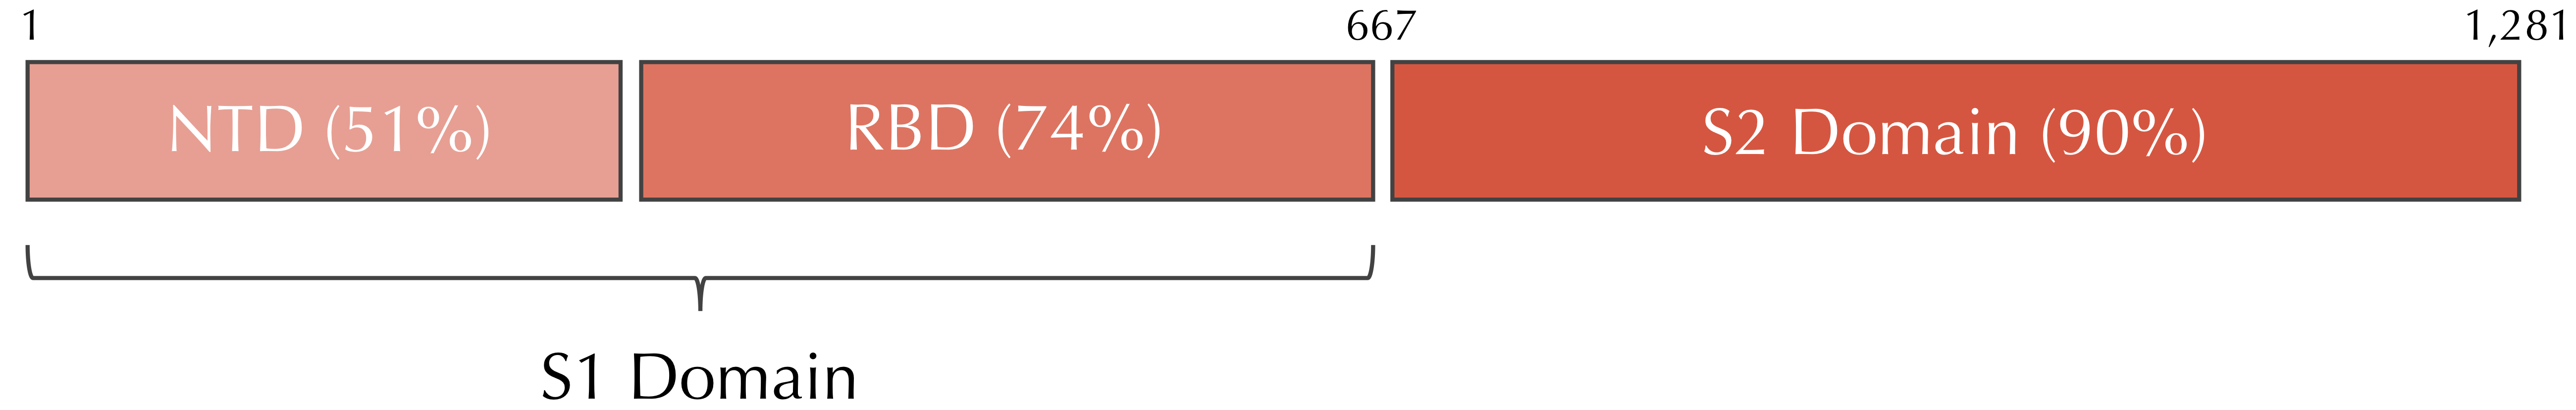
\includegraphics[width = 0.7\textwidth]{../images/spike_protein_similarity.png}
	\caption{Variable and conserved regions in the SARS-CoV and SARS-CoV-2 spike proteins. The S1 domain tends to be more variable, whereas the S2 domain is more conserved (and even has a small region of 100\% similarity). In this figure, "NTD" stands for "N-terminal domain" and "RBD" stands for "receptor binding domain", two subunits of the S1 domain. Source: Jaimes et al. 2020.}
	\label{fig:spike_protein_similarity}
\end{figure}

Some homology modeling algorithms account for variable and conserved regions by assuming that very conserved regions in the two genes correspond to essentially identical structures in the proteins. That is, the structure of our protein of interest in these regions will be the same as those of the template protein. We can then use a \textdef{fragment library}{fragment library}{FILL IN}, a catalog of known substructures from many proteins, to fill in the structure of non-conserved regions based on structures of fragments whose sequence is similar to these regions. This approach is called \textdef{fragment assembly}{fragment assembly}{FILL IN}.

We will model the SARS-CoV-2 spike protein using homology modeling software from three publicly available servers (SWISS-MODEL, Robetta, and GalaxyWEB), all of which apply a variant of fragment assembly. If the results are similar, then we have faith in the \textit{robustness} of our predictions to using different approaches. Furthermore, comparing the results of multiple different approaches may give us more insights into structure prediction. \tutorial[https://biologicalmodeling.org/coronavirus/tutorial_homology]

\FloatBarrier
\phantomsection
\subsection{Applying homology modeling to the SARS-CoV-2 spike protein}

The results of the three software resources for predicting the structure of the SARS-CoV-2 spike protein are available for download in \autoref{fig:homology_modeling_results_table}.

\begin{figure}[h]
\centering
\tabcolsep = 1 em
\mySfFamily
\begin{tabular}{c c}
\textbf{Structure Prediction Sever} & \textbf{Results} \\
SWISS-MODEL (spike protein) & \url{https://biologicalmodeling.org/_pages/coronavirus/files/SWISS_Model.zip} \\
Robetta (Single-Chain spike protein) & \url{https://biologicalmodeling.org/_pages/coronavirus/files/Robetta_Model.zip} \\
GalaxyWEB & \url{https://biologicalmodeling.org/_pages/coronavirus/files/GalaxyWEB_Models.zip} \\
\end{tabular}
\caption{A table containing the download link for the prediction results of three homology modeling softwares. SWISS-MODEL was used to predict the structure of the SARS-CoV-2 spike protein. Robetta was used to predict the structure of a single chain of the SARS-CoV-2 spike protein. GalaxyWEB was used to predict the structure of the receptor binding domain (RBD) of the SARS-CoV-2 spike protein.}
\label{fig:homology_modeling_results_table}
\end{figure}

o compare the protein structures resulting from running software on the SARS-CoV-2 spike protein sequence, we need a way to represent a protein's tertiary structure. In `.pdb` format (shown in \autoref{fig:simplifiedPDB}), each atom in the protein is labeled according to several different pieces of information, including:

1. the element from which the atom derives;
2. the amino acid in which the atom is contained;
3. the chain on which this amino acid is found;
4. the position of the amino acid within this chain; and
5. the 3D coordinates (*x*, *y*, *z*) of the atom in angstroms ($$10^{-10}$$ meters).

\begin{figure}[h]
	\centering
	\mySfFamily
	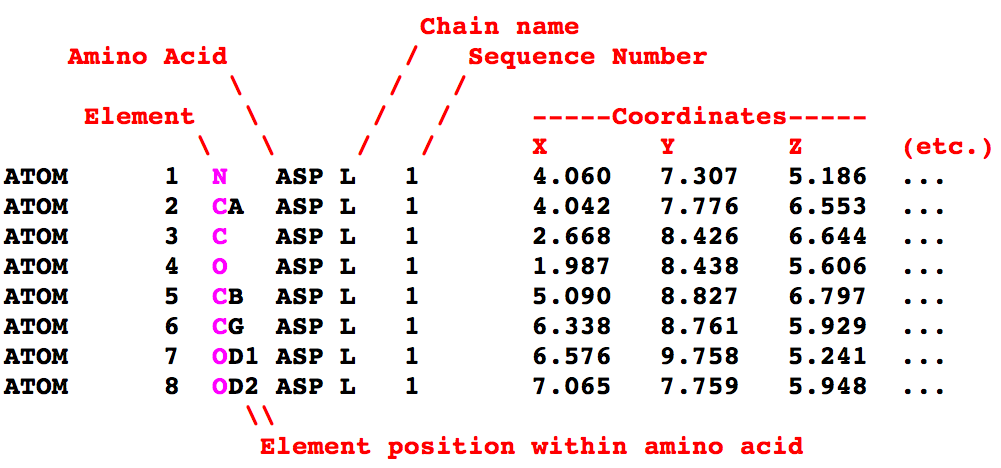
\includegraphics[width = 0.7\textwidth]{../images/simplifiedPDB.png}
	\caption{A simplified diagram showing how the \texttt{.pdb} format encodes the 3D coordinates of every atom while labeling the identity of this atom and the chain on which it is found. Source: https://proteopedia.org/wiki/index.php/Atomic_coordinate_file}
	\label{fig:simplifiedPDB}
\end{figure}

\begin{note}[%
The above figure shows just part of the information needed to fully represent a protein structure. For example, a \texttt{.pdb} file will also contain information about the disulfide bonds between amino acids. For more information, check out the <a href="http://www.wwpdb.org/documentation/file-format" target="_blank">official PDB documentation</a>).
]\end{note}

Now that we can represent protein structures, we wish to compare two protein structures. How similar are the three predicted structures of the SARS-CoV-2 spike protein to each other, and how similar are they to the structure of the SARS-CoV spike protein? This is a simple question, but it has a complicated answer, to which we will devote an entire section.

\FloatBarrier
\phantomsection

\section{Ab initio Protein Structure Prediction}
\label{sec:accuracy}
\phantomsection
\subsection{Experiments determine the structure of the SARS-CoV-2 spike protein}

While some scientists were working to predict the structure of the SARS-CoV-2 spike protein from sequence data, others were working on verifying the structure of this protein experimentally. On February 25, 2020, researchers from the Seattle Structural Genomics Center for Infectious Disease uploaded to the PDB the result of a cryo-EM experiment for the SARS-CoV-2 spike protein, which became entry 6vxx (\url{http://www.rcsb.org/structure/6VXX}).

\begin{note}[%
If you would like to explore the structure of the SARS-CoV-2 spike protein, check out the 3-D protein viewer at \url{http://www.rcsb.org/3d-view/6VXX/1}
]\end{note}

In this section, we will compare the results of the SARS-CoV-2 spike protein prediction from the previous section against each other and against the protein's empirically validated structure. To do so, we need a method of comparing two structures.

\FloatBarrier
\phantomsection
\subsection{Comparing two shapes with the Kabsch algorithm}

Ultimately, comparing protein structures is intrinsically similar to comparing two shapes, such as those shown in \autoref{fig:two_shapes}.

\begin{qbox}[%
Consider the two shapes in \autoref{fig:two_shapes}. How similar are they?
]\end{qbox}

\begin{figure}[h]
	\centering
	\mySfFamily
	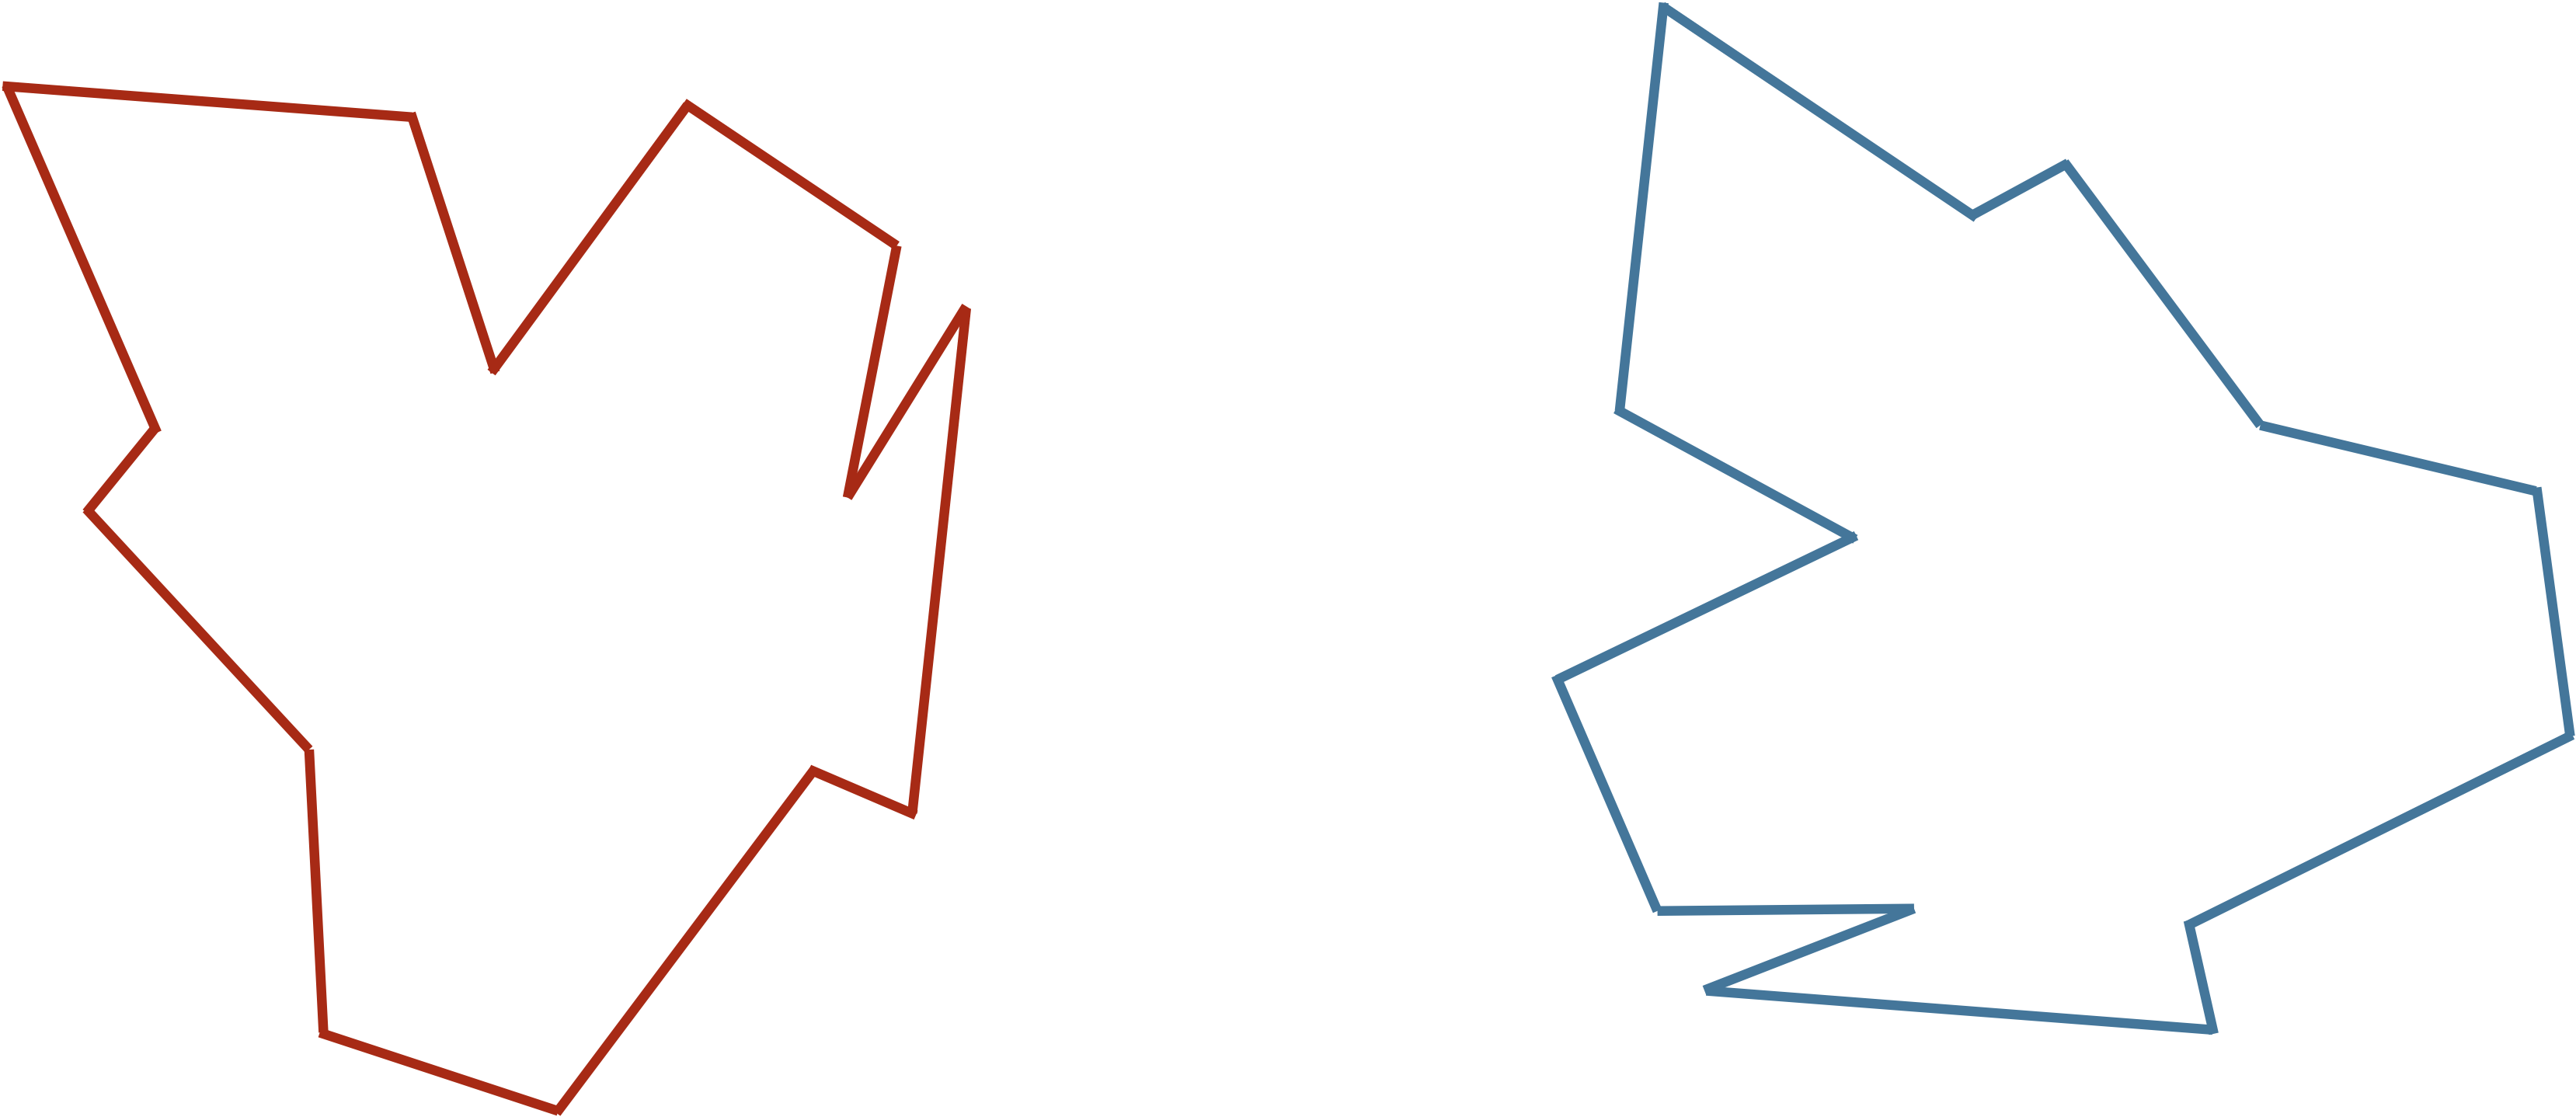
\includegraphics[width = 0.7\textwidth]{../images/two_shapes.png}
	\caption{Two simple shapes.}
	\label{fig:two_shapes}
\end{figure}

If you think you have a good handle on comparing the two shapes in \autoref{fig:two_shapes}, then it is because humans have very highly evolved eyes and brains. As we will see in the next chapter, training a computer to see objects as well as we can is more difficult than you think!

We would like to develop a "distance function $d(S, T)$ quantifies how different two shapes $S$ and $T$ are. If $S$ and $T$ are the same, then $d(S, T)$ should be equal to zero; the more different the shapes, the larger $d$ should become.

You may have noticed that the two shapes in the preceding figure are similar; in fact, they are identical. To demonstrate that this is true, we can first move the red shape to superimpose it over the blue shape, then flip the red shape, and finally rotate it so that its boundary coincides with the blue shape.

\texttt{NEED FIGURE HERE -- TO REPLACE GIF}\\
% (../assets/images/shape_transformations.gif)
% We can transform the red shape into the blue shape by translating it, flipping it, and then rotating it.

If $S$ can be translated, flipped, and/or rotated to produce $T$, then $S$ and $T$ are the same shape, and so $d(S, T)$ should be equal to zero. The question is what $d(S, T)$ should be if $S$ and $T$ are not the same shape.

Our idea for defining $d(S, T)$ is first to translate, flip, and rotate $S$ so that it resembles $T$ "as much as possible" to give us a fair comparison. We will then to quantify how different the shapes are to determine $d(S, T)$.

We first translate $S$ to have the same \textdef{centroid}{centroid}{FILL IN} (or \textdef{center of mass}{center of mass}{FILL IN}) as $T$. The centroid of $S$ is found at the point $(x_{S}, y_{S})$ such that $x_{S}$ and $y_{S}$ are the respective averages of the \textit{x}-coordinates and \textit{y}-coordinates on the boundary of $S$.

For example, suppose that $S$ is the semicircular arc shown in \autoref{fig:semicircular_arc}, with endpoints $(-1, 0)$ and $(1, 0)$.

\begin{figure}[h]
	\centering
	\mySfFamily
	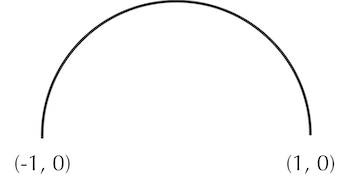
\includegraphics[width = 0.7\textwidth]{../images/semicircular_arc.png}
	\caption{A semicircular arc with radius 1 corresponding to a circle whose center is at the origin.}
	\label{fig:semicircular_arc}
\end{figure}

The \textit{x}-coordinate $x_{S}$ is zero, but computing $y_{S}$ requires us to apply a little calculus, taking the average of the \textit{y}-coordinates along the entire semicircle:

$$y_S & = \dfrac{\int_{0}^{\pi}{\sin{\theta}}}{\pi} \\
& = \dfrac{-\cos{\pi} + \cos{0}}{\pi} \\
& = \dfrac{2}{\pi}$$

\begin{qbox}[%
Say that we connect $(-1, 0)$ and $(0, 1)$ to form a closed semicircle. What will be the centroid of the resulting shape?
]\end{qbox}

The centroid of some shapes, like the semicircular arc in the preceding example, can be determined mathematically. But for irregular shapes, we can estimate the centroid of $S$ by sampling $n$ points from the boundary of the shape and taking the averages of all the \textit{x}- and \textit{y}-coordinates of sampled points.

After finding the centroids of the two shapes $S$ and $T$ that we wish to compare, we translate $S$ so that it has the same centroid as $T$. We then wish to find the rotation of $S$, possibly along with a flip as well, that makes the shape resemble $T$ as much as possible.

Imagine that we have found the desired rotation; we can then define $d(S, T)$ in the following way. We sample $n$ points along the boundary of each shape, converting $S$ and $T$ into \textdef{vectors}{vectors}{FILL IN} $s = (s_{1}, \cdots, s_{n})$ and $t = (t_{1}, \cdots, t_{n})$, where $s_{i}$ is the $i$-th point on the boundary of $S$. The \textdef{root mean square deviation (RMSD)}{root mean square deviation (RMSD)}{FILL IN} between the two shapes is the square root of the average squared distance between corresponding points in the vectors,

$$\text{RMSD}(s, t) = \sqrt{\dfrac{1}{n} \cdot (d(s_1, t_1)^2 + d(s_2, t_2)^2 + \cdots + d(s_n, t_n)^2)}\,. $$

In this formula, $d(s_{i}, t_{i})$ is the distance between the points $s_{i}$ and $t_{i}$.

\begin{note}[%
RMSD is a very commonly used approach across data science when measuring the differences between two vectors.
]\end{note}

For an example two-dimensional RMSD calculation, consider \autoref{fig:rmsd_simple_shapes}, which shows two shapes with four points sampled from each.

\begin{figure}[h]
	\centering
	\mySfFamily
	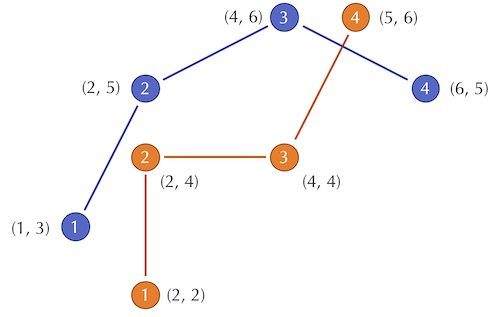
\includegraphics[width = 0.7\textwidth]{../images/rmsd_simple_shapes.png}
	\caption{Two shapes with four points sampled from each.}
	\label{fig:rmsd_simple_shapes}
\end{figure}

The distances between corresponding points in this figure are equal to $\sqrt{2}$, 1, 4, and $\sqrt{2}$. As a result, we compute the RMSD as

$$\text{RMSD}(s, t) & = \sqrt{\dfrac{1}{4} \cdot (\sqrt{2}^2 + 1^2 + 2^2 + \sqrt{2}^2)} \\
& = \sqrt{\dfrac{1}{4} \cdot 9}\\
& = \sqrt{\dfrac{9}{4}}\\
& = \dfrac{3}{2}$$

\begin{qbox}[%
Do you see any issues with using RMSD to compare two shapes?
]\end{qbox}

Even if we assume that the shapes have already been overlapped and rotated appropriately, we still need to make sure that we sample enough points to give a good approximation of how different the shapes are. Consider a circle inscribed within a square, as shown in \autoref{fig:circle_square_undersampling}. If we happened to sample only the four points indicated, then we would sample the same points for each shape and conclude that the RMSD between these two shapes is equal to zero. Fortunately, this issue is easily resolved by making sure to sample enough points to avoid approximation errors.

\begin{figure}[h]
	\centering
	\mySfFamily
	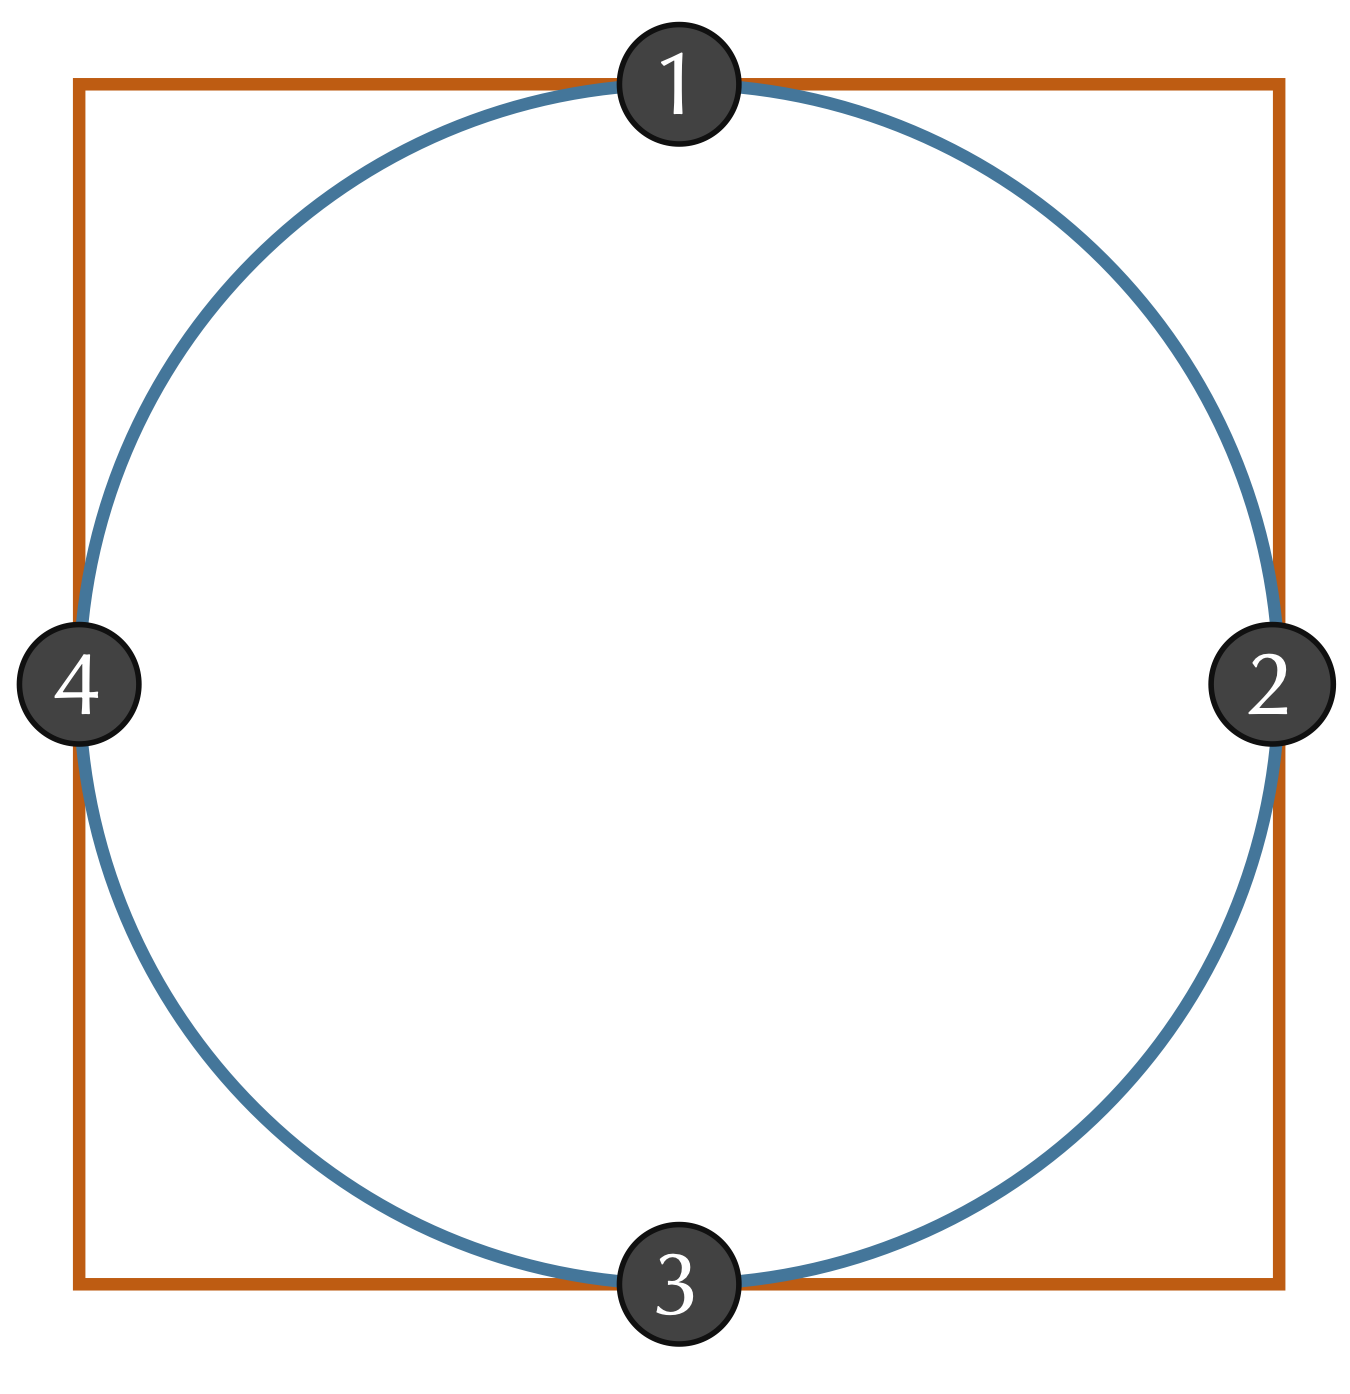
\includegraphics[width = 0.7\textwidth]{../images/circle_square_undersampling.png}
	\caption{A circle inscribed within a square. Sampling of the four points where the shapes intersect will give a flawed estimate of zero for RMSD.}
	\label{fig:circle_square_undersampling}
\end{figure}

However, we have still assumed that we already rotated (and possibly flipped) $S$ to be as "similar" to $T$ as possible. In practice, after superimposing $S$ and $T$ to have the same centroid, we will find the flip and/or rotation of $S$ that \textit{minimizes} the RMSD between our vectorizations of $S$ and $T$ over all possible ways of flipping and rotating $S$. It is this minimum RMSD that we define as $d(S, T)$.

The best way of rotating and flipping $S$ so as to minimize the RMSD between the resulting vectors $s$ and $t$ can be found with a method called the \textdef{Kabsch algorithm}{Kabsch algorithm}{FILL IN}. Explaining this algorithm requires some advanced linear algebra and is beyond the scope of our work but is described at \url{https://en.wikipedia.org/wiki/Kabsch_algorithm}.

\FloatBarrier
\phantomsection
\subsection{Applying the Kabsch algorithm to protein structure comparison}

The Kabsch algorithm offers a compelling way to determine the similarity of two protein structures. We can convert a protein containing $n$ amino acids into a vector of length $n$ by selecting a single representative point from each amino acid. We typically use the alpha carbon, the amino acid's centrally located carbon atom; the position of this atom will be present in the \texttt{.pdb} file for a given structure.

\begin{qbox}[%
Can you think of an example in which a small difference between protein structures can cause a large inflation in RMSD score?
]\end{qbox}

Unfortunately, the Kabsch algorithm can be flawed. Consider \autoref{fig:RMSD_weakness_mutation} showing two toy protein structures. The orange structure ($S$) is identical to the blue structure ($T$) except for a change in a single bond angle between the third and fourth amino acids. And yet this tiny change in the protein's structure causes a significant increase in $d(s_{i}, t_{i}) for every $i$ greater than 3, which inflates the RMSD.

\begin{figure}[h]
	\centering
	\mySfFamily
	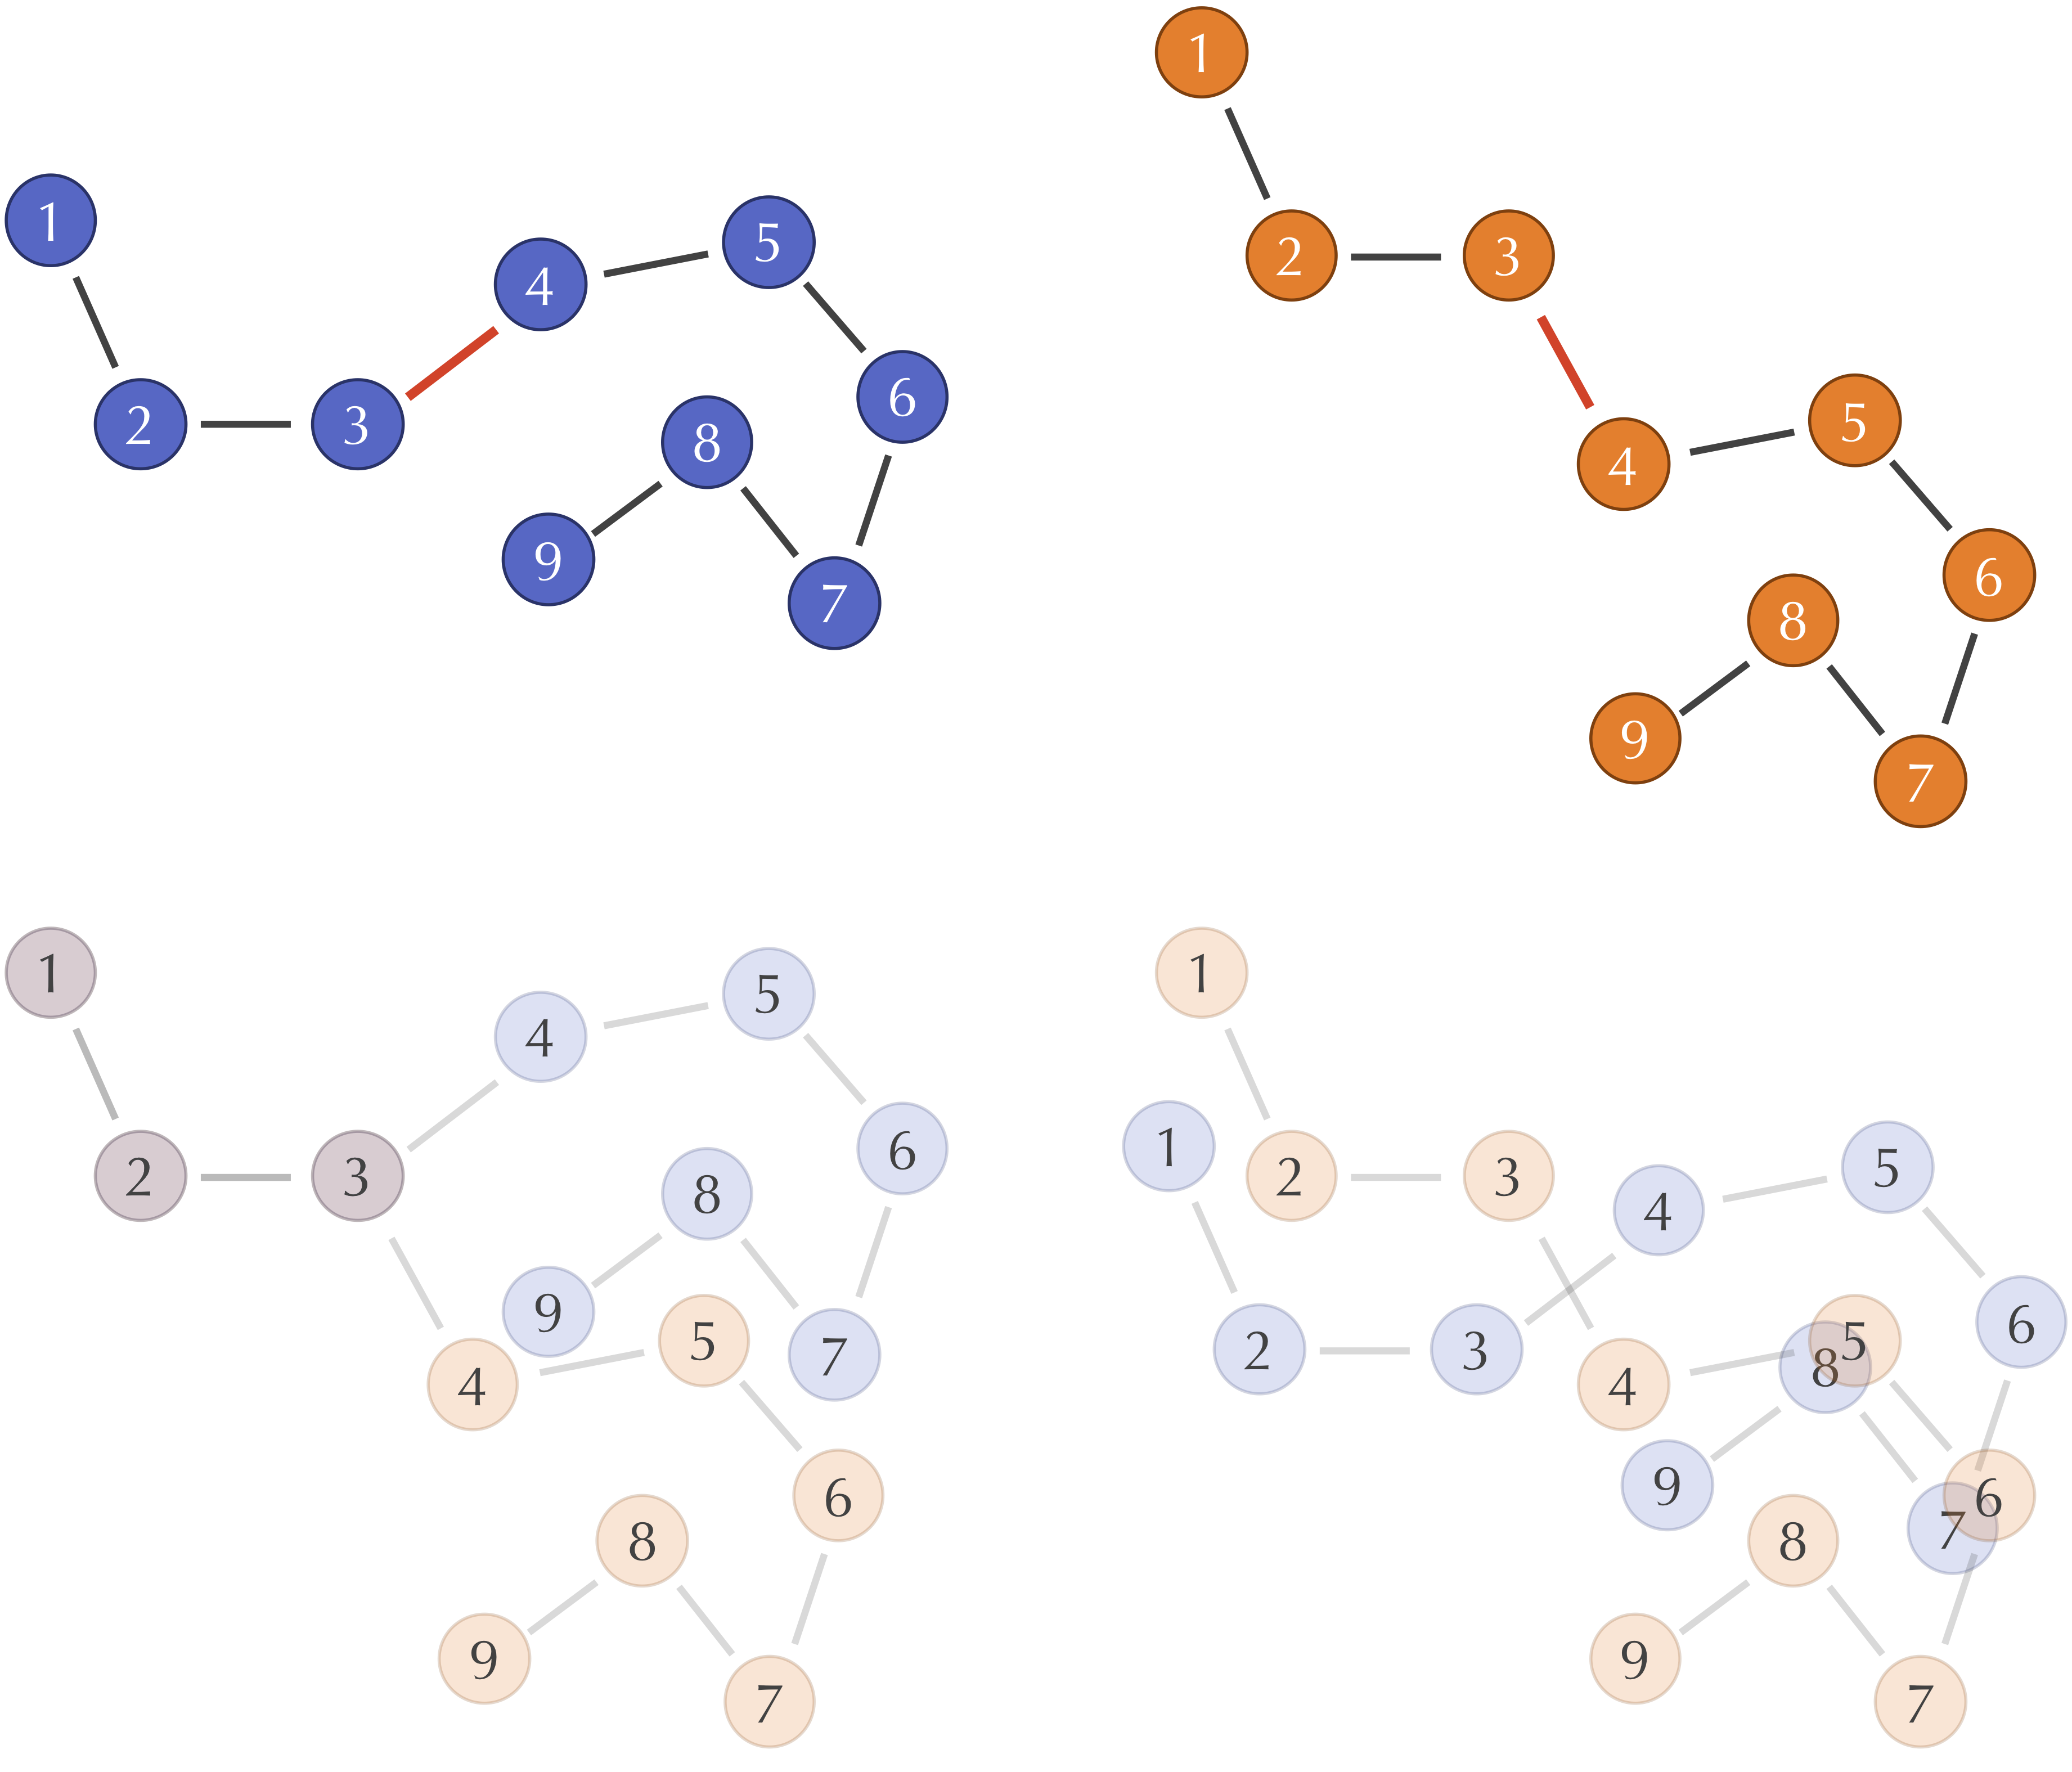
\includegraphics[width = 0.7\textwidth]{../images/RMSD_weakness_mutation.png}
	\caption{(Top) Two hypothetical protein structures that differ in only a single bond angle between the third and fourth amino acids, shown in red. Each circle represents an alpha carbon. (Bottom left) Superimposing the first three amino acids shows how much the change in the bond angle throws off the computation of RMSD by increasing the distances between corresponding alpha carbons. (Bottom right) The Kabsch algorithm would align the centers of gravity of the two structures in order to minimize RMSD between corresponding alpha carbons. This alignment belies the similarity in the structures and makes it difficult for the untrained observer to notice that the two proteins only really differ in a single bond angle.}
	\label{fig:RMSD_weakness_mutation}
\end{figure}

Another way in which the Kabsch algorithm can be fooled is in the case of an appended substructure that throws off the ordering of the amino acids. \autoref{fig:RMSD_weakness_loop} shows a toy example of a structure into which we incorporate a loop, thus throwing off the natural order of comparing amino acids. (The same effect is caused if one or more amino acids are deleted from one of the two proteins.)

\begin{figure}[h]
	\centering
	\mySfFamily
	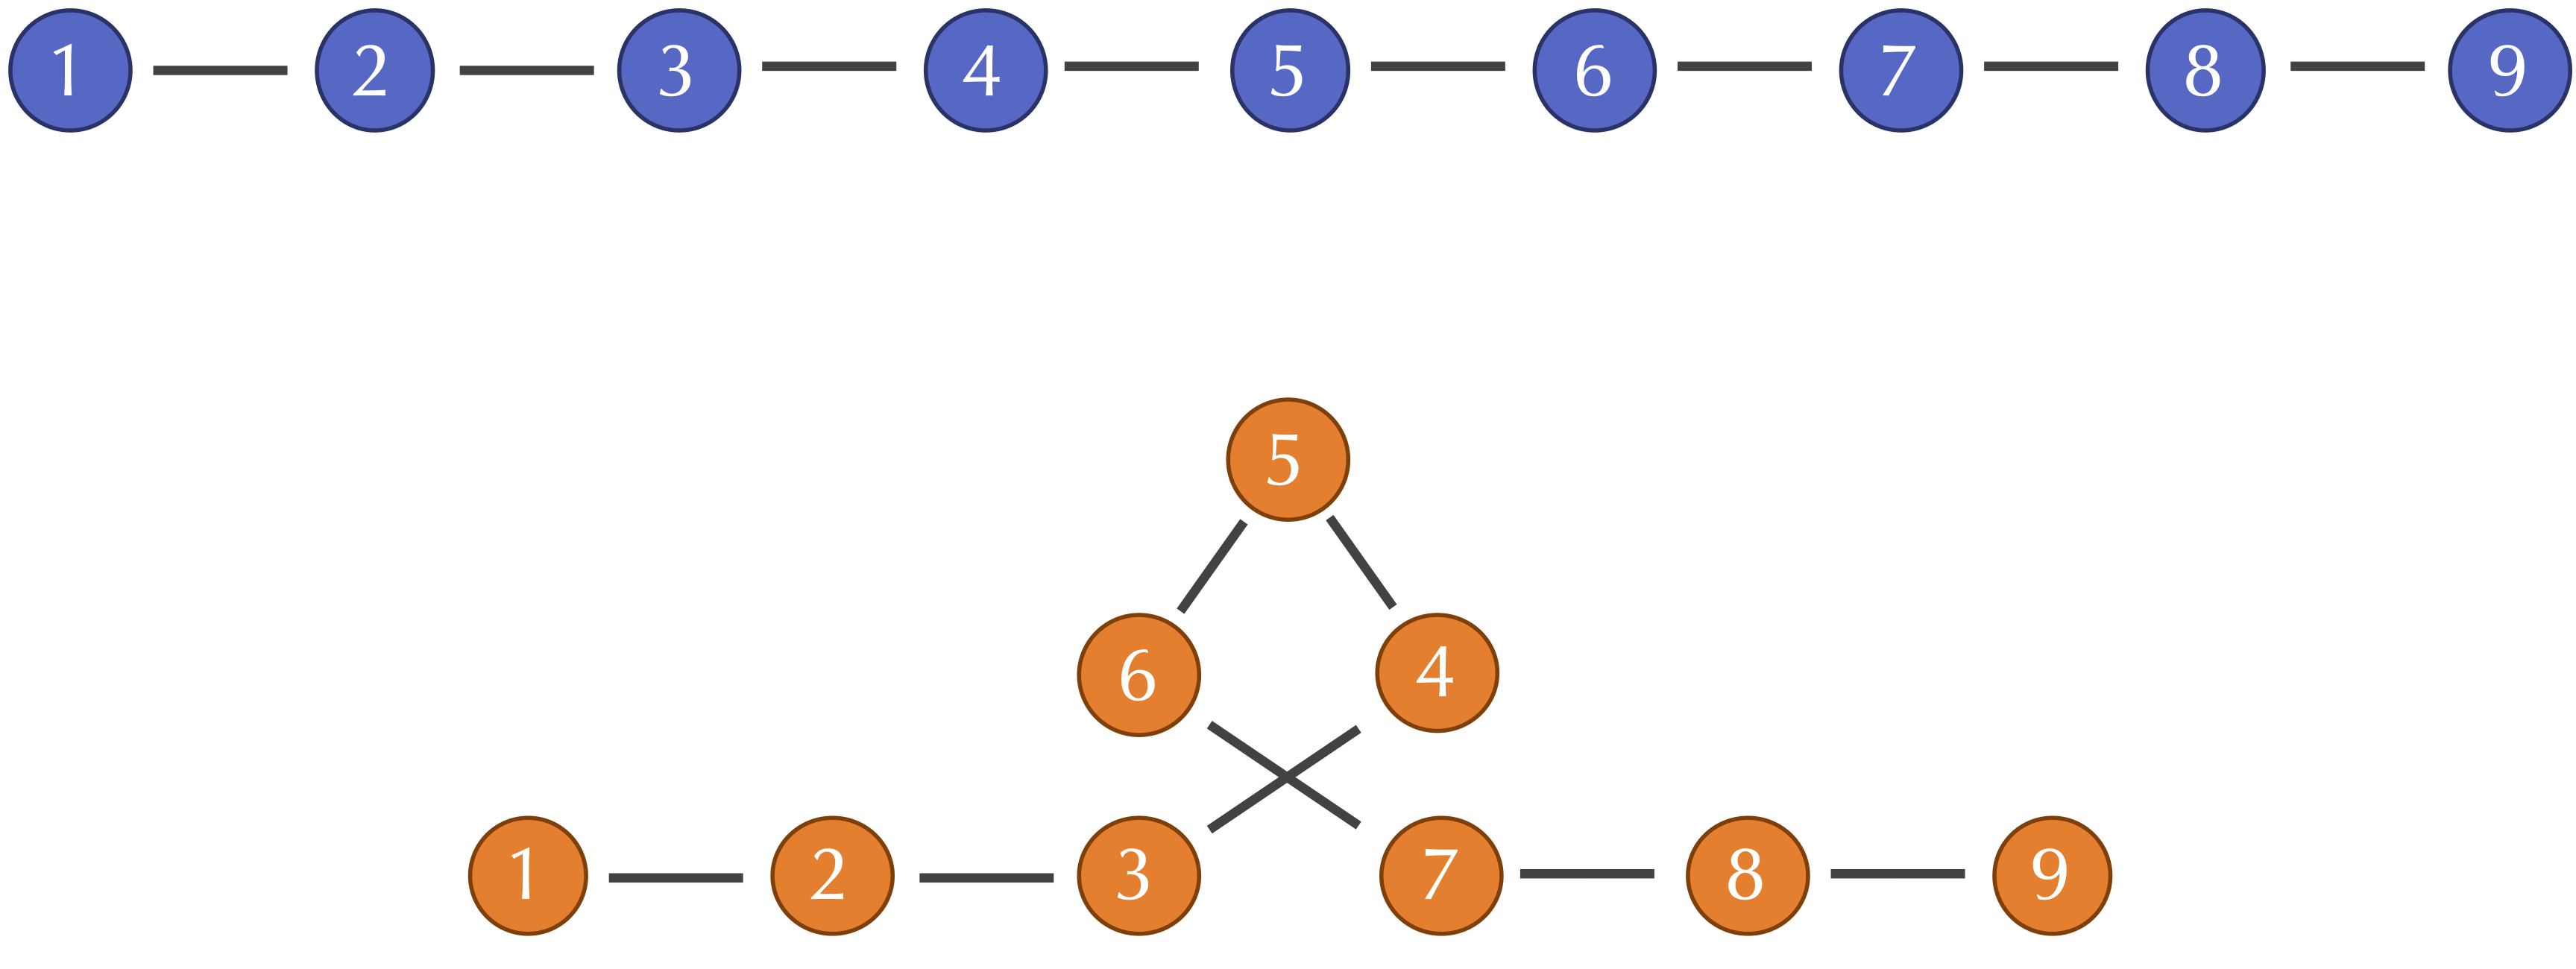
\includegraphics[width = 0.7\textwidth]{../images/RMSD_weakness_loop.png}
	\caption{A simplification of two protein structures, one of which includes a loop of three amino acids. After the loop, each amino acid in the orange structure will be compared against an amino acid that occurs farther long in the blue structure, thus increasing $d(s_{i}, t_{i})^2$ for each such amino acid.}
	\label{fig:RMSD_weakness_loop}
\end{figure}

To address these shortcomings, biologists will often align the sequences of two proteins first, discarding any positions that do not align well when it comes time to perform the RMSD calculation. We will soon see an example of a protein sequence alignment soon when comparing the coronavirus spike proteins.

In short, if the RMSD of two proteins is \textit{large}, then we should be wary of concluding that the proteins are very different, and we may need to combine RMSD with other methods of structure comparison. But if the RMSD is \textit{small} (e.g., just a few angstroms), then we can have confidence that the proteins are indeed similar.

We are now ready to apply the Kabsch algorithm to compare the structures that we predicted for human hemoglobin subunit alpha and the SARS-CoV-2 spike protein against their experimentally validated structures. \tutorial[https://biologicalmodeling.org/coronavirus/tutorial_rmsd]

\FloatBarrier
\phantomsection
\subsection{Assessing the accuracy of our structure prediction models}

In the tutorials occurring earlier in this module, we used publicly available protein structure prediction servers to predict the structure of human hemoglobin subunit alpha (using \textit{ab initio} modeling) and the SARS-CoV-2 spike protein (using homology modeling).

Let's see how well our models performed by showing the values of RMSD produced by the Kabsch algorithm when comparing each of these models against the validated structures.

\FloatBarrier
\phantomsection
\subsection{\textit{Ab initio} (QUARK) models of Human Hemoglobin Subunit Alpha}

We previously showed that QUARK (https://zhanglab.ccmb.med.umich.edu/QUARK/) produced five predicted structures from the amino acid sequence of human hemoglobin subunit alpha. \autoref{fig:quark_rmsd_table} shows the RMSD given by the Kabsch algorithm for each of these models against the validated structure of this subunit (PDB:1si4).

\begin{figure}[h]
\centering
\tabcolsep = 1 em
\mySfFamily
\begin{tabular}{c c}
\textbf{QUARK Models} & \textbf{RMSD} \\
QUARK1 & 1.58 \\
QUARK2 & 2.0988 \\
QUARK3 & 3.11 \\
QUARK4 & 1.9343 \\
QUARK5 & 2.6495 \\
\end{tabular}
\caption{A table containing the the calculated RMSD of the QUARK models of human hemoglobin subunit alpha compared to the validated structure (PDB entry:1si4).}
\label{fig:quark_rmsd_table}
\end{figure}

It is tempting to conclude that our \textit{ab initio} prediction was a success. However, because human hemoglobin subunit alpha is such a short protein (141 amino acids), researchers would consider this RMSD score high.

We know that homology modeling will be faster than \textit{ab initio} modeling. But will it be more accurate as well?

\FloatBarrier
\phantomsection
\subsection{Homology models of SARS-CoV-2 spike protein}

In \tutorial[https://biologicalmodeling.org/coronavirus/tutorial_homology], we used SWISS-MODEL and Robetta to predict the structure of the SARS-CoV-2 spike protein, and we used GalaxyWeb to predict the structure of this protein's receptor binding domain (RBD). In addition to our predicted models, we will also assess five predicted models of the full SARS-CoV-2 spike protein released early in the COVID-19 pandemic by Rosetta@Home (\url{https://boinc.bakerlab.org/}) and published to the Seattle Structural Genomics Center for Infectious Disease (SSGCID).

Because the work needed to generate these models was distributed over many users' machines, comparing the RMSD scores obtained by the Rosetta@Home models against our own may provide insights on the effect of computational power on the accuracy of predictions. The SSGCID models are publically available on their website (\url{https://www.ssgcid.org/cttdb/molecularmodel_list/?target__icontains=BewuA}).

\FloatBarrier
\phantomsection
\subsection{GalaxyWEB}

First, we consider the five GalaxyWEB (\url{http://galaxy.seoklab.org/}) models produced for the spike protein RBD. \autoref{fig:galaxyweb_rmsd_table} shows the RMSD between each of these models and the validated SARS-CoV-2 RBD (PDB entry: 6lzg).

\begin{figure}[h]
\centering
\tabcolsep = 1 em
\mySfFamily
\begin{tabular}{c c}
\textbf{GalaxyWEB Models} & \textbf{RMSD} \\
Galaxy1 & 0.1775 \\
Galaxy2 & 0.1459 \\
Galaxy3 & 0.1526 \\
Galaxy4 & 0.1434 \\
Galaxy5 & 0.1202 \\
\end{tabular}
\caption{A table containing the the calculated RMSD of the GalaxyWEB models of SARS-CoV-2 spike protein RBD compared to the validated structure (PDB entry:6lzg).}
\label{fig:galaxyweb_rmsd_table}
\end{figure}

All of these models have an excellent RMSD score and can be considered very accurate. Note that their RMSD is more than an order of magnitude lower than the RMSD computed for our \textit{ab initio} model of hemoglobin subunit alpha, despite the fact that the RBD is longer (229 amino acids).

\FloatBarrier
\phantomsection
\subsection{SWISS-MODEL}

We now shift to homology models of the entire spike protein and start with SWISS-MODEL (\url{https://swissmodel.expasy.org/}). \autoref{fig:swiss_rmsd_table} shows the RMSD between each of three structures produced by SWISS-MODEL and the validated structure of the SARS-CoV-2 spike protein (PDB entry: 6vxx).

\begin{figure}[h]
\centering
\tabcolsep = 1 em
\mySfFamily
\begin{tabular}{c c}
\textbf{SWISS-MODEL Models} & \textbf{RMSD} \\
SWISS1 & 5.8518 \\
SWISS2 & 11.3432 \\
SWISS3 & 11.3432 \\
\end{tabular}
\caption{A table containing the the calculated RMSD of the SWISS-MODEL models of SARS-CoV-2 spike protein compared to the validated structure (PDB entry:6vxx).}
\label{fig:swiss_rmsd_table}
\end{figure}

The first structure has a lowest RMSD over the three models, and even though its RMSD (5.818) is significantly higher than what we saw for the GalaxyWEB prediction for the RBD, keep in mind that the spike protein is 1281 amino acids long, and so the sensitivity of RMSD to slight changes should give us confidence that our models are on the right track.

\FloatBarrier
\phantomsection
\subsection{Robetta}

Finally, we produced five predicted structures of a single chain of the SARS-CoV-2 spike protein using Robetta (\url{https://robetta.bakerlab.org/}). \autoref{fig:robetta_rmsd_table} compares each of them against the validated structure of the SARS-CoV-2 spike protein (PDB entry: 6vxx).

\begin{figure}[h]
\centering
\tabcolsep = 1 em
\mySfFamily
\begin{tabular}{c c}
\textbf{Robetta Models} & \textbf{RMSD} \\
Robetta1 & 0.1775 \\
Robetta2 & 0.1459 \\
Robetta3 & 0.1526 \\
Robetta4 & 0.1434 \\
Robetta5 & 0.1202 \\
\end{tabular}
\caption{A table containing the the calculated RMSD of the Robetta models of SARS-CoV-2 spike protein chain A compared to the validated structure (PDB entry:6vxx).}
\label{fig:robetta_rmsd_table}
\end{figure}

\begin{qbox}[%
Which do you think performed more accurately on our predictions: SWISS-MODEL or Robetta?
]\end{qbox}

\FloatBarrier
\phantomsection
\subsection{SSGCID}

As explained previously, the SSGCID models of the spike protein released by Rosetta@Home (\url{https://boinc.bakerlab.org/}) used large amounts of computational resources. Therefore, we might expect to see RMSD scores lower than those of our models. Like before, we will compare the models to the validated structure of (PDB entry: 6vxx). This time, we will assess the accuracy of predictions of a single chain as well as of the entire spike protein.

\begin{figure}[h]
\centering
\tabcolsep = 1 em
\mySfFamily
\begin{tabular}{c c c}
\textbf{SSGCID Models} & \textbf{RMSD (Full Protein} & \textbf{RMSD (Single Chain)} \\
SSGCID1  & 3.505 & 2.7843 \\
SSGCID2  & 2.3274 & 2.107 \\
SSGCID3  & 2.12 & 1.866 \\
SSGCID4  & 2.0854 & 2.047 \\
SSGCID5  & 4.9636 & 4.6443 \\
\end{tabular}
\caption{A table containing the the calculated RMSD of the SSGCID models of SARS-CoV-2 spike protein, full protein and single chain, compared to the validated structure (PDB entry:6vxx).}
\label{fig:ssgcid_rmsd_table}
\end{figure}

As we might expect due to their access to the resources of thousands of users' computers, the SSGCID models outperform our SWISS-MODEL models. Yet a typical threshold for whether a predicted structure is accurate is if its RMSD compared to a validated structure is smaller than 2.0 angstroms, and the SSGCID models are not quite this accurate, even with access to hundreds of contributors' machines.

The inability of the SSGCID models to attain a very accurate predicted structure may make it seem that protein structure prediction is a lost cause. Perhaps biochemists should head back to expensive experimental validations and ignore the musings of computational scientists. In the conclusion to part 1, we will find hope.

\FloatBarrier
\phantomsection

\section{Part 1 Conclusion: Protein Structure Prediction is Solved! (Kind of…)}
\label{sec:conclusion_part_1}
\phantomsection

In 1967, the Soviets founded an entire research insitute (\url{https://www.protres.ru}) dedicated to protein research and decoding nature's magic protein folding algorithm. Most of its founding scientists are dead now, but the institute carries on.

Protein structure prediction is an old problem, but continual algorithmic improvements and increasing computational resources have led biologists around the world to wish for the day when they could consider protein structure prediction to be solved.

That day has come. Kind of.

Every two years since 1994, a global effort called \textdef{Critical Assessment of protein Structure Prediction (CASP)}{Critical Assessment of protein Structure Prediction (CASP)}{FILL IN} has allowed modelers to test their protein structure prediction algorithms against each other. The contest organizers compile a (secret) collection of experimentally verified protein structures and then run all submitted algorithms against these proteins.

The 14th iteration of this contest, held in 2020, was won in a landslide. The second version of AlphaFold (\url{https://deepmind.com/blog/article/alphafold-a-solution-to-a-50-year-old-grand-challenge-in-biology}), one of the projects of DeepMind (an Alphabet subsidiary), vastly outperformed the world's foremost structure prediction approaches, including those that we discussed in this module.

The algorithm powering AlphaFold is an extremely involved method based on deep learning, a topic that we will discuss in this work's final module. If you're interested in learning more about this algorithm, consult the AlphaFold website or this excellent blog post by Mohammed al Quraishi: \url{https://bit.ly/39Mnym3}.

Instead of using RMSD, CASP scores a predicted structure against a known structure using the \textdef{global distance test (GDT)}{global distance test (GDT)}{FILL IN}. For some threshold $t$, we first take the percentage of alpha carbon positions for which the distance between corresponding alpha carbons in the two structures is at most $t$. The GDT score that CASP uses then averages the percentages obtained when $t$ is equal to each of 1, 2, 4, and 8 angstroms. A GDT score of 90\% is considered good, and a score of 95\% is considered excellent (i.e., comparable to minor errors resulting from experimentation).

We will show a few plots to illustrate the decisiveness of AlphaFold's CASP victory. The first graph, which is shown in \autoref{fig:AlphaFold2_BAKER}, compares the scores of AlphaFold against the second-place algorithm (a product of David Baker's laboratory, which developed the Robetta and Rosetta@Home software that we used in this module).

\begin{figure}[h]
	\centering
	\mySfFamily
	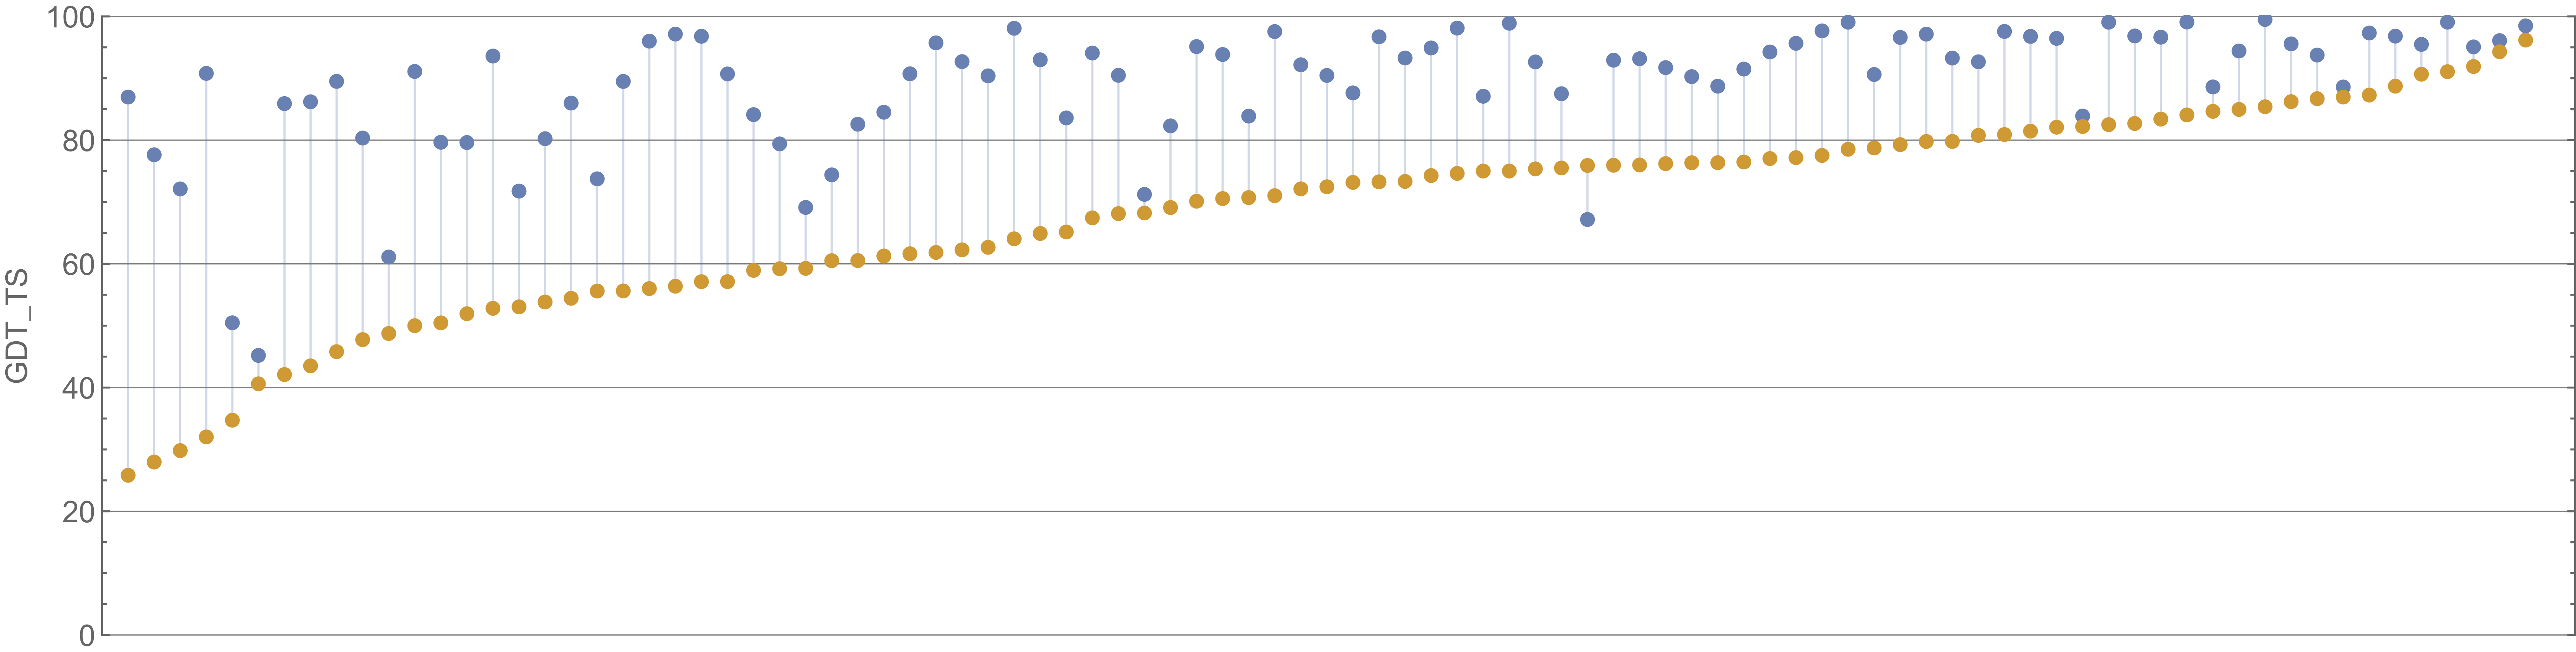
\includegraphics[width = 0.7\textwidth]{../images/AlphaFold2_BAKER.png}
	\caption{A plot of GDT scores for AlphaFold2 (shown in blue) and Baker lab (shown in orange) submissions over all proteins in the CASP14 contest. AlphaFold2 finished first in CASP14, and Baker lab finished second. Image courtesy: Mohammed al Quraishi (\url{https://bit.ly/39Mnym3}).}
	\label{fig:AlphaFold2_BAKER}
\end{figure}

We can appreciate the margin of victory in the above figure if we compare it against the margin between the second- and third-place competitors, shown in \autoref{fig:BAKER_Zhang}

\begin{figure}[h]
	\centering
	\mySfFamily
	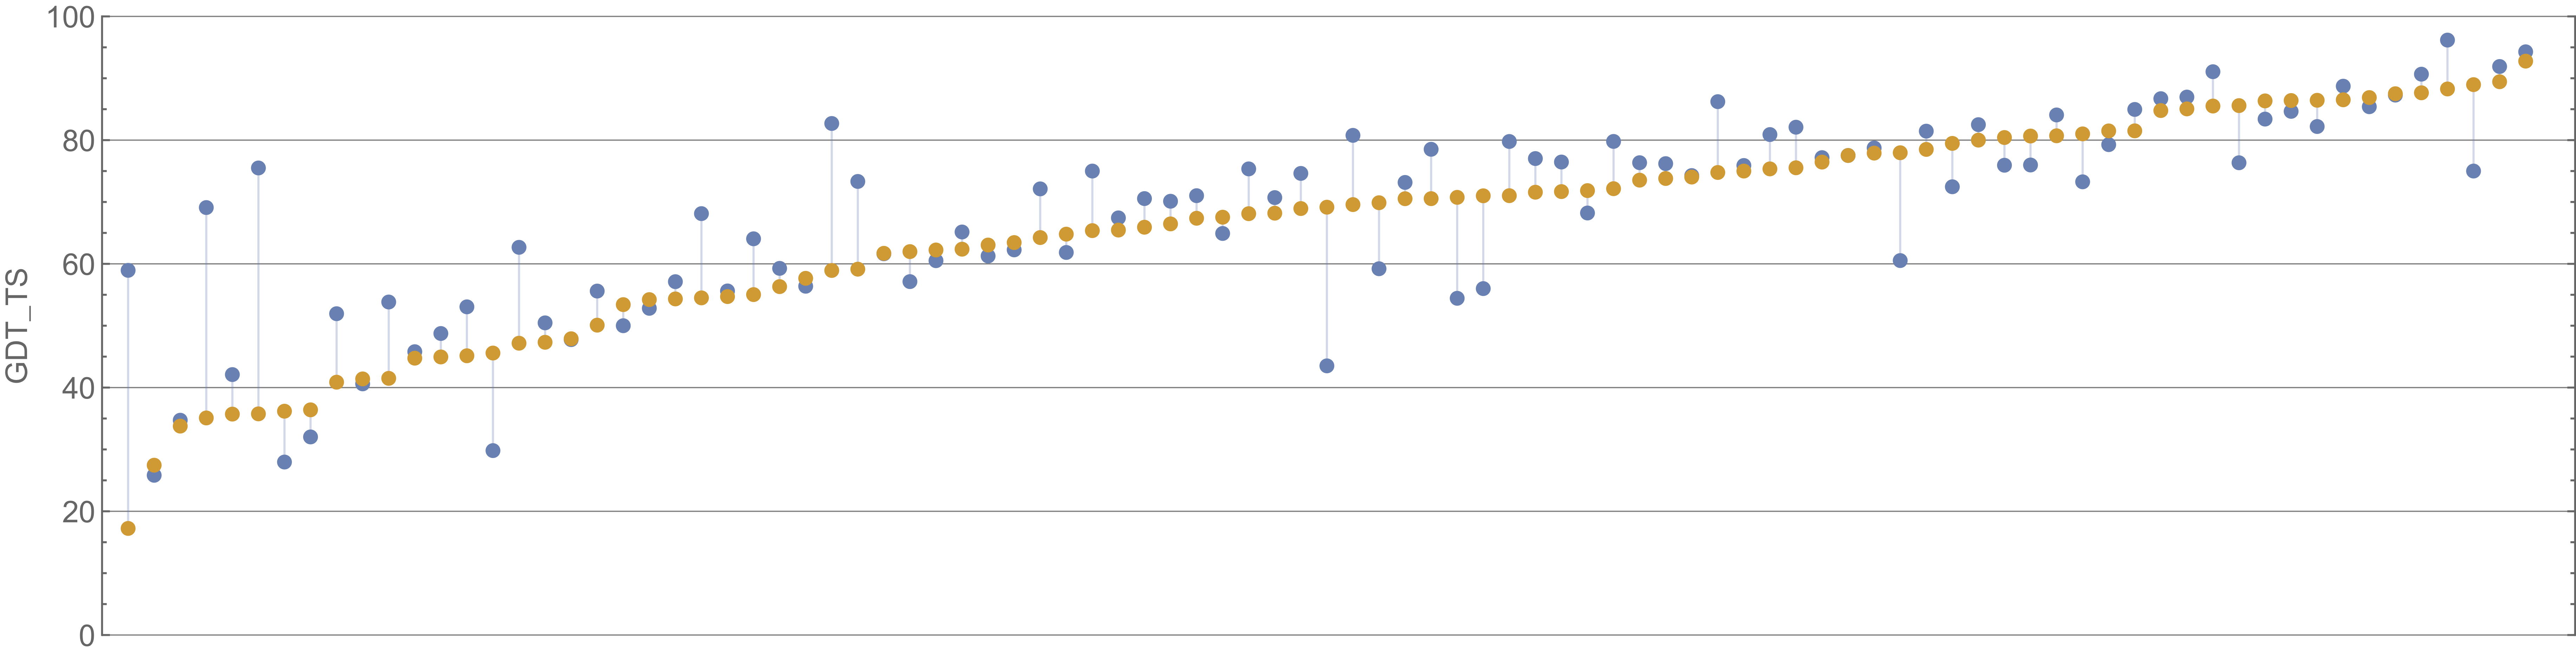
\includegraphics[width = 0.7\textwidth]{../images/BAKER_Zhang.png}
	\caption{A plot of GDT scores for the Baker lab (shown in blue) and Zhang lab (shown in orange) submissions for all proteins in the CASP14 contest. Baker lab finished second in CASP14, and Zhang lab finished third. Image courtesy: Mohammed al Quraishi (\url{https://bit.ly/39Mnym3}).}
	\label{fig:BAKER_Zhang}
\end{figure}

For each protein in the CASP14 contest, we can also compute each algorithm's \textdef{z-score}{z-score}{FILL IN}, defined as the number of standard deviations that the algorithm's GDT score falls from the mean GDT score over all competitors. For example, a z-score of 1.4 would imply that the approach performed 1.4 standard deviations above the mean, and a z-score of -0.9 would imply that the approach performed 0.9 standard deviations below the mean.

By summing all of an algorithm's positive z-scores, we obtain a reasonable metric for the relative quality of an algorithm compared to its competitors. If an algorithm's sum of z-scores is large, then the algorithm racked up lots of positive z-scores, and we can conclude that it performed well. \autoref{fig:CASP14_overall_results} shows the sum of z-scores for all CASP14 participants and reiterates the margin of AlphaFold's victory.

\begin{figure}[h]
	\centering
	\mySfFamily
	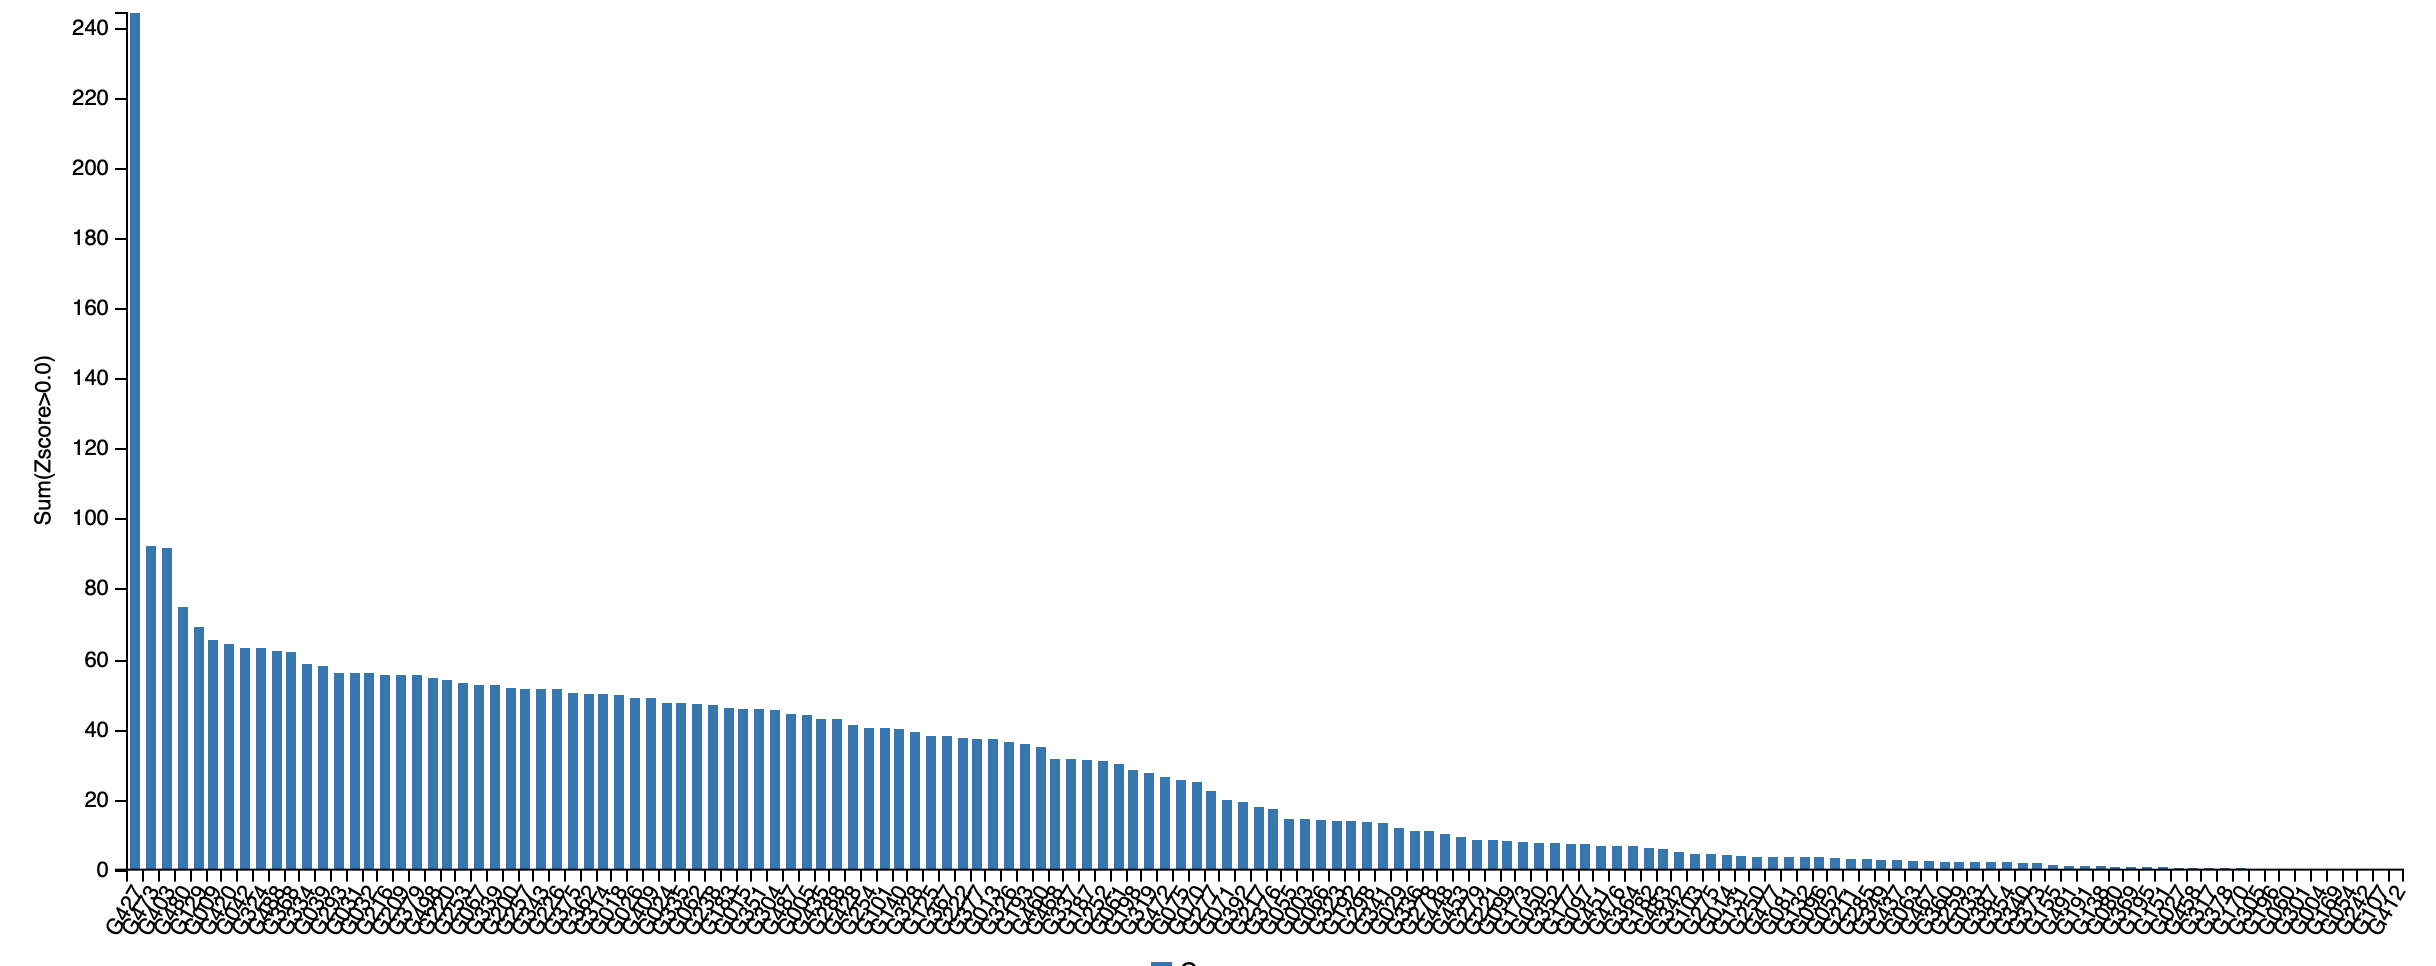
\includegraphics[width = 0.7\textwidth]{../images/CASP14_overall_results.png}
	\caption{A bar chart plotting the sum of z-scores for every entrant in the CASP14 contest. AlphaFold2 is shown on the far left; its sum of z-scores is over double that of the second-place submission. Source: https://predictioncenter.org/casp14/zscores_final.cgi.}
	\label{fig:CASP14_overall_results}
\end{figure}

AlphaFold's CASP14 victory led some scientists --- and media outlets --- to declare that protein structure prediction had finally been solved. Yet some critics remained skeptical.

AlphaFold obtained an impressive median RMSD of 1.6 angstroms for its predicted proteins, but to be completely trustworthy for a sensitive application like designing drug targets, a predicted protein structure would need to have an RMSD nearly an order of magnitude lower.

Furthermore, about a third of AlphaFold's CASP14 predictions have an RMSD over 2.0 angstroms, which we mentioned in the previous section is often used as a threshold for whether a predicted structure is reliable. And there is no way of knowing in advance whether AlphaFold will perform well on a given protein, unless we validate the protein's structure. For example, AlphaFold published their predictions of the structures of other SARS-CoV-2 proteins, none of which had validated structures in 2020. Most of these predictions are probably accurate, but we cannot know for sure without experimentation.

Finally, the AlphaFold algorithm is "trained" using a database of known protein structures, which makes it more likely to succeed if a protein is similar to a known structure. But it is the proteins with structures \textit{dissimilar} to any known structure that possess some of the greatest scientific interest.

Pronouncing protein structure prediction to be solved may be hasty, but we will likely never again see such a clear improvement to the state of the art for structure prediction. AlphaFold is probably the final great innovation in a research problem that has puzzled biologists for fifty years.

Thus ends part 1 of this chapter, but there is still much for us to discuss. We hope that you will join us for part 2, in which we will delve further into measuring the differences between the spike proteins of SARS-CoV and SARS-CoV-2 using the validated protein structures published to PDB early in the pandemic.

\FloatBarrier
\phantomsection

\section{Finding Local Differences in Protein Structures with Qres}
\label{sec:multiseq}
\phantomsection

In part 1 of this chapter, we used a variety of existing software resources to predict the structure of the SARS-CoV-2 spike protein from its amino acid sequence. We then discussed how to compare our predicted structures against the experimentally confirmed structure of the protein.

Now begins part 2, in which we examine how the structure of the SARS-CoV-2 spike protein compares against the SARS-CoV spike protein. In keeping with the biological maxim that the \textit{structure} of a protein informs the \textit{function} of that protein, can we find any clues lurking in the spike proteins' structure that would indicate why the two viruses had different fates?

\FloatBarrier
\phantomsection
\subsection{Focusing on a variable region of interest in the spike protein}

In part 1, we saw that the spike protein is much more variable than other regions of the viral genomes. We even see variable and conserved regions within the spike protein, as \autoref{fig:spike_protein_similarity} (reproduced from \autoref{sec:homology} indicates.

\begin{figure}[h]
	\centering
	\mySfFamily
	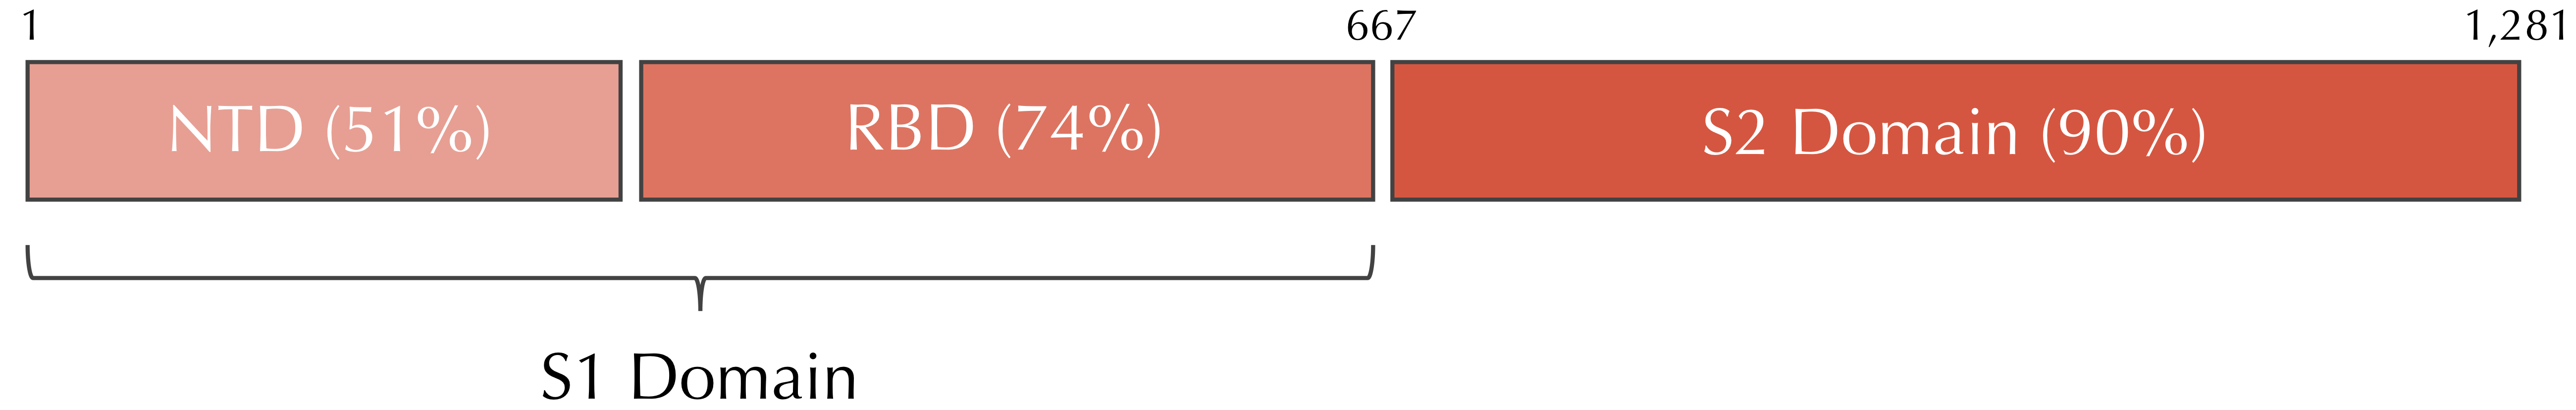
\includegraphics[width = 0.7\textwidth]{../images/spike_protein_similarity.png}
	\caption{Variable and conserved regions in the SARS-CoV and SARS-CoV-2 spike proteins. The S1 domain tends to be more variable, whereas the S2 domain is more conserved (and even has a small region of 100\% similarity). In this figure, "NTD" stands for "N-terminal domain" and "RBD" stands for "receptor binding domain", two subunits of the S1 domain. Source: Jaimes et al. 2020.}
	\label{}
\end{figure}

The most variable region between the two viruses in the spike protein is the \textdef{receptor binding motif (RBM)}{receptor binding motif (RBM)}{FILL IN}, part of the receptor binding domain (RBD) whose structure we predicted using GalaxyWEB in the \tutorial[https://biologicalmodeling.org/coronavirus/tutorial_homology]. The RBM is the component of the RBD that mediates contact with ACE2, as the following simplified animation of the process illustrates.

\texttt{NEED FIGURE HERE -- TO REPLACE VIDEO}\\
% include video id="e2Qi-hAXdJo" provider="youtube" %

The fact that the region binding to the target human enzyme has mutated so much makes it a fascinating region of study. Do the mutations that SARS-CoV-2 has accumulated somehow make it easier for the virus to infect human cells?

As we hone in on the RBM, \autoref{fig:RBM_alignment} shows an alignment of the 70 amino acid long RBM region from SARS-CoV and SARS-CoV-2.

\begin{figure}[h]
	\centering
	\mySfFamily
	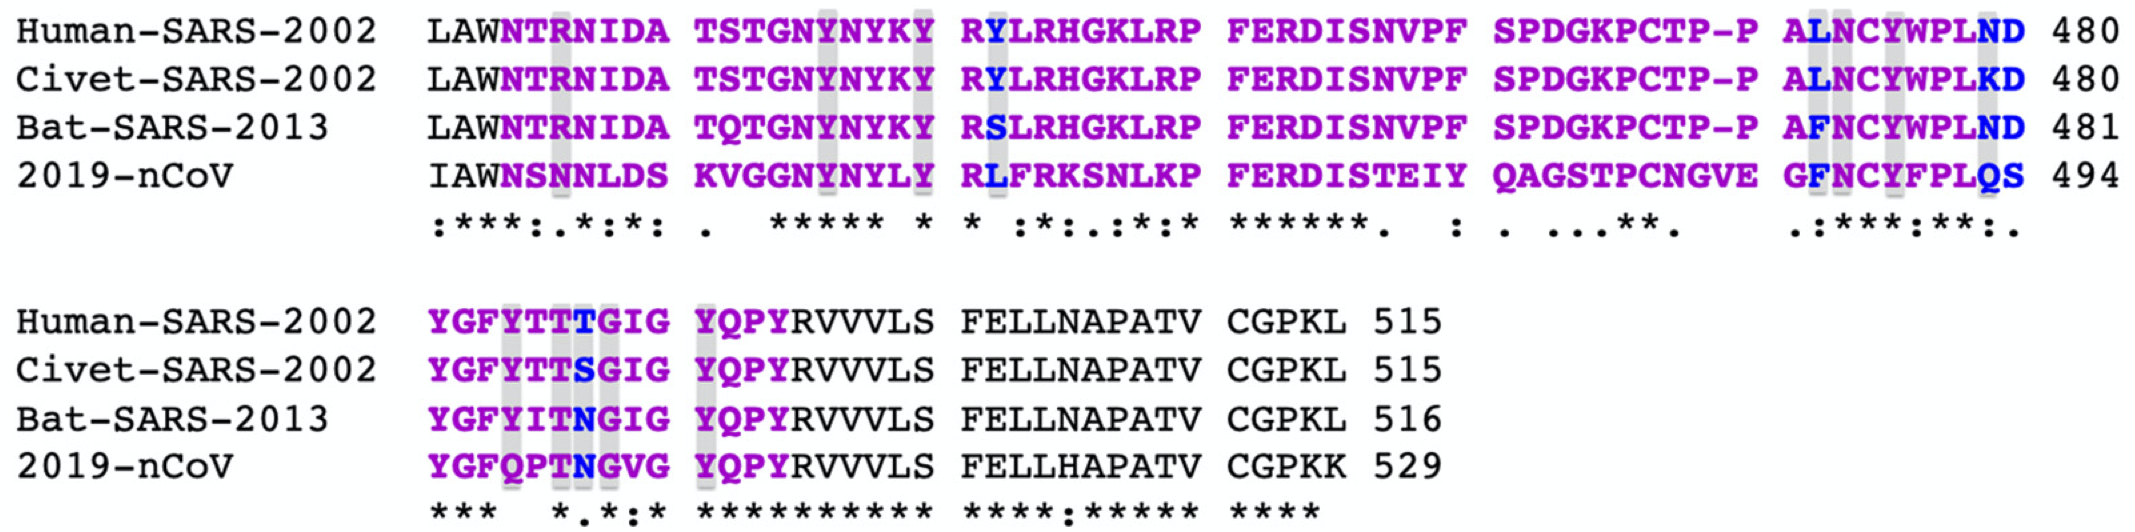
\includegraphics[width = 0.7\textwidth]{../images/RBM_alignment.png}
	\caption{An alignment of the RBM of the human SARS-CoV virus (first row) and the SARS-CoV-2 virus (second row). Amino acids that are highlighted in green represents matches between the two sequence. Beneath each column is the conservation between the two sequences, where full conservation indicates a match and partial conservation indicates a mismatch.}
	\label{fig:RBM_alignment}
\end{figure}

We know from our work in structure prediction that just because the sequence of a protein has been greatly mutated does not mean that the structure of that protein has changed much. Therefore, in this section, we will start a structural comparison of the SARS-CoV and SARS-CoV-2 spike proteins. All of this analysis will be performed using the software resources ProDy and VMD.

\FloatBarrier
\phantomsection
\subsection{Using bound spike-ACE2 enzymes}

In addition to verifying the structure of the spike protein in both SARS-CoV and SARS-CoV-2, researchers also determined the structure of the RBD complexed with ACE2 in both SARS-CoV (PDB entry: 2ajf and SARS-CoV-2 (PDB entry: 6vw1).

\begin{note}[%
	The experimentally verified SARS-CoV-2 structure is a \textit{chimeric} protein formed of the SARS-CoV RBD in which the RBM has the sequence from SARS-CoV-2 (Shang et al. 2020). A chimeric RBD was used for complex technical reasons to ensure that the crystallization process during X-ray crystallography could be borrowed from that used for SARS-CoV.
]\end{note}

Because we know the structures of the bound complexes, we can produce 3-D visualizations of the two different complexes and look for structural differences involving the RBM. We will use VMD to produce this visualization, rotating the structures around to examine potential differences. However, we should be wary of only trusting our eyes to guide us; can we use a computational approach to tell us where to look for structural differences between the two RBMs?

\FloatBarrier
\phantomsection
\subsection{A first attempt at identifying local dissimilarities between protein structures}

To assess the accuracy of a predicted structure, we introduced a metric called root mean square deviation (RMSD) for quantifying the difference between two protein structures. RMSD offered an excellent method for a \textit{global} comparison (i.e., a comparison across all structures), but we are interested in the \textit{local} regions where the SARS-CoV and SARS-CoV-2 complexes differ. To this end, we will need an approach that considers individual amino acids in similar protein structures.

\begin{qbox}[%
	How could we compare individual amino acid differences of two protein structures?
]\end{qbox}

Recall the following definition of RMSD for two protein structures $s$ and $t$, in which each structure is represented by the positions of its $n$ alpha carbons $(s_{1}, \cdots, s_{n})$ and $(t_{1}, \cdots, t_{n})$.

$$\text{RMSD}(s, t) = \sqrt{\dfrac{1}{n} \cdot (d(s_1, t_1)^2 + d(s_2, t_2)^2 + \cdots + d(s_n, t_n)^2)}\,. $$

If two similar protein structures differ in a few locations, then the corresponding alpha carbon distances $d(s_{i}, t_{i})$ will likely be higher at these locations. However, we will introduce a more sophisticated approach for
comparing the local structure of $s_{i}$ against $t_{i}$. First, however, we will discuss an alternative to RMSD for computing global structure.

\FloatBarrier
\phantomsection
\subsection{Contact maps and Qres}

One of the weaknesses of RMSD that we pointed out in part 1 of this module is that a change to a single bond angle at the $i$-th position may cause $d(s_{j}, t_{j})$ to be nonzero when $j > i$, even though the structure of the protein downstream of this bond angle has not changed. For example, when we discussed the Kabsch algorithm in \autoref{sec:accuracy}, we showed \autoref{fig:single_bond_angle} of two protein structures that are identical except for a single bond angle. All of the alpha carbon distances $d(s_{i}, t_{i})$ for $i$ at least equal to 4 will be thrown off by this changed angle.

\begin{figure}[h]
	\centering
	\mySfFamily
	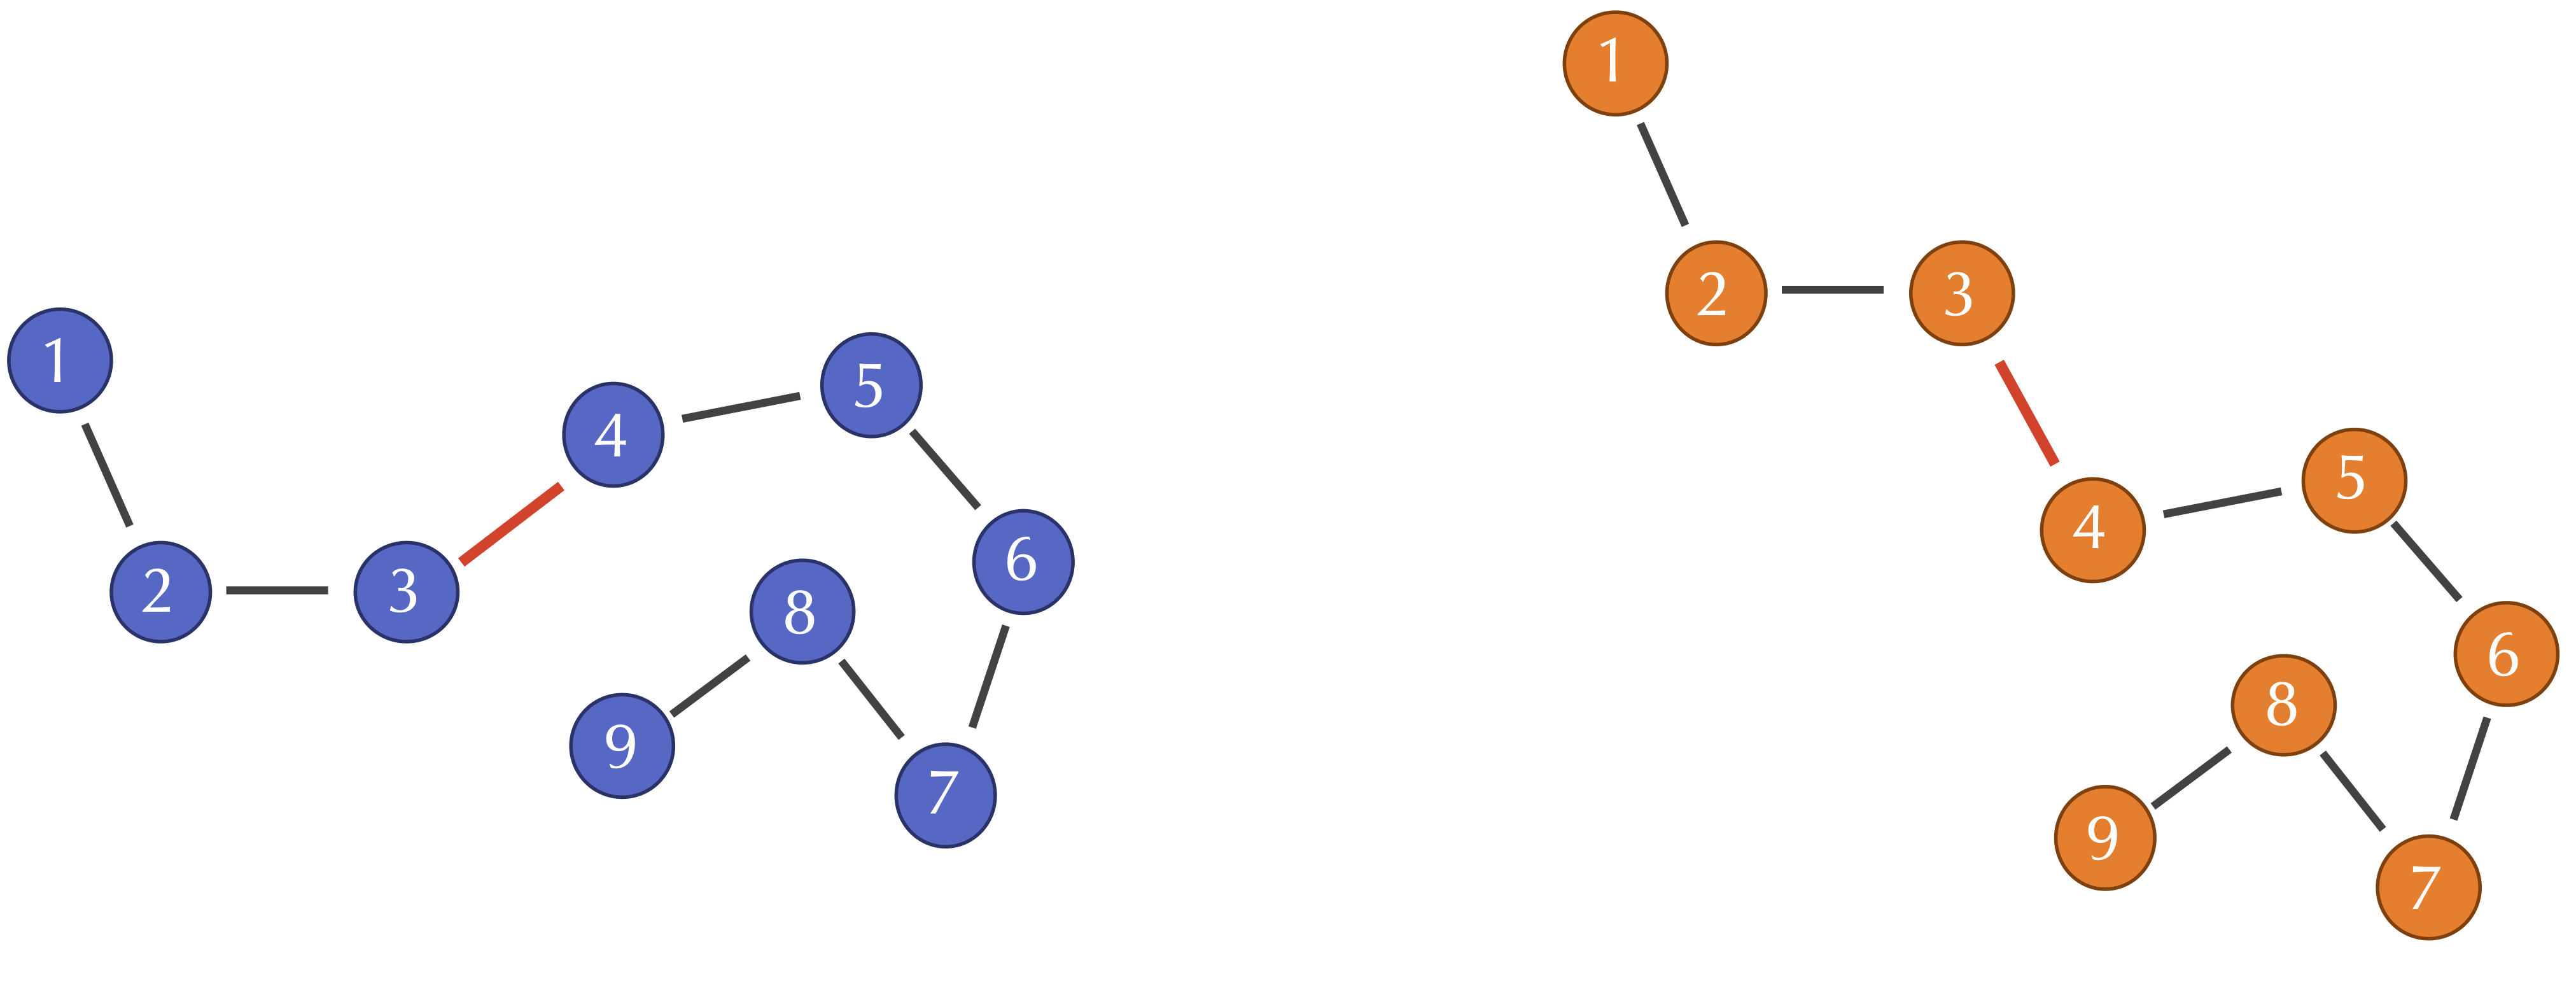
\includegraphics[width = 0.7\textwidth]{../images/single_bond_angle.png}
	\caption{Two toy protein structures in which the bond angle between the third and fourth alpha carbon has been changed. This change does not affect the distance between the \textit{i}-th and \textit{j}-th alpha carbons when \textit{i} and \textit{j} are both at least equal to 4.}
	\label{fig:single_bond_angle}
\end{figure}

However, note that when $i$ and $j$ are both at least equal to 4, the distance $d(s_{i}, s_{j})$ between the $i$-th and $j$-th alpha carbons in $S$ will still be similar to the distance $d(t_{i}, t_{j})$ between the same alpha carbons in $T$. This observation leads us to a more robust approach for measuring differences in two protein structures, which compares \textit{all} pairwise distances $d(s_{i}, s_{j})$ in one protein structure against the corresponding distances $d(t_{i}, t_{j})$ in the other structure.

To help us visualize all these pairwise distances, we will introduce the \textdef{contact map}{contact map}{FILL IN} of a protein structure, which is a binary matrix indicating whether two alpha carbons are near each other. After setting a threshold distance, for a given structure $s$, we set $M(i, j) = 1$ if the distance $d(s_{i}, s_{j})$ is less than the threshold, and $M(i, j) = 0$ if $d(s_{i}, s_{j})$ is greater than or equal to the threshold.

\autoref{fig:Contact} shows the contact maps for the SARS-CoV-2 and SARS-CoV spike proteins (both full proteins and single chains) with a threshold distance of twenty angstroms. In this map, we color contact map values black if they are equal to 1 (close amino acid pairs) and white if they are equal to 0 (distant amino acid pairs).

We note two things in the contact maps in \autoref{fig:Contact}. First, many black values cluster around the main diagonal of the matrix, since amino acids that are nearby in the protein sequence will remain near each other in the 3-D structure. Second, the contact maps for the two proteins are very similar, reinforcing that the two proteins have similar structures.

\begin{note}[%
	Interested in learning how to make contact maps? We will use ProDy to do so in a later section.
]\end{note}

\begin{figure}[h]
	\centering
	\mySfFamily
	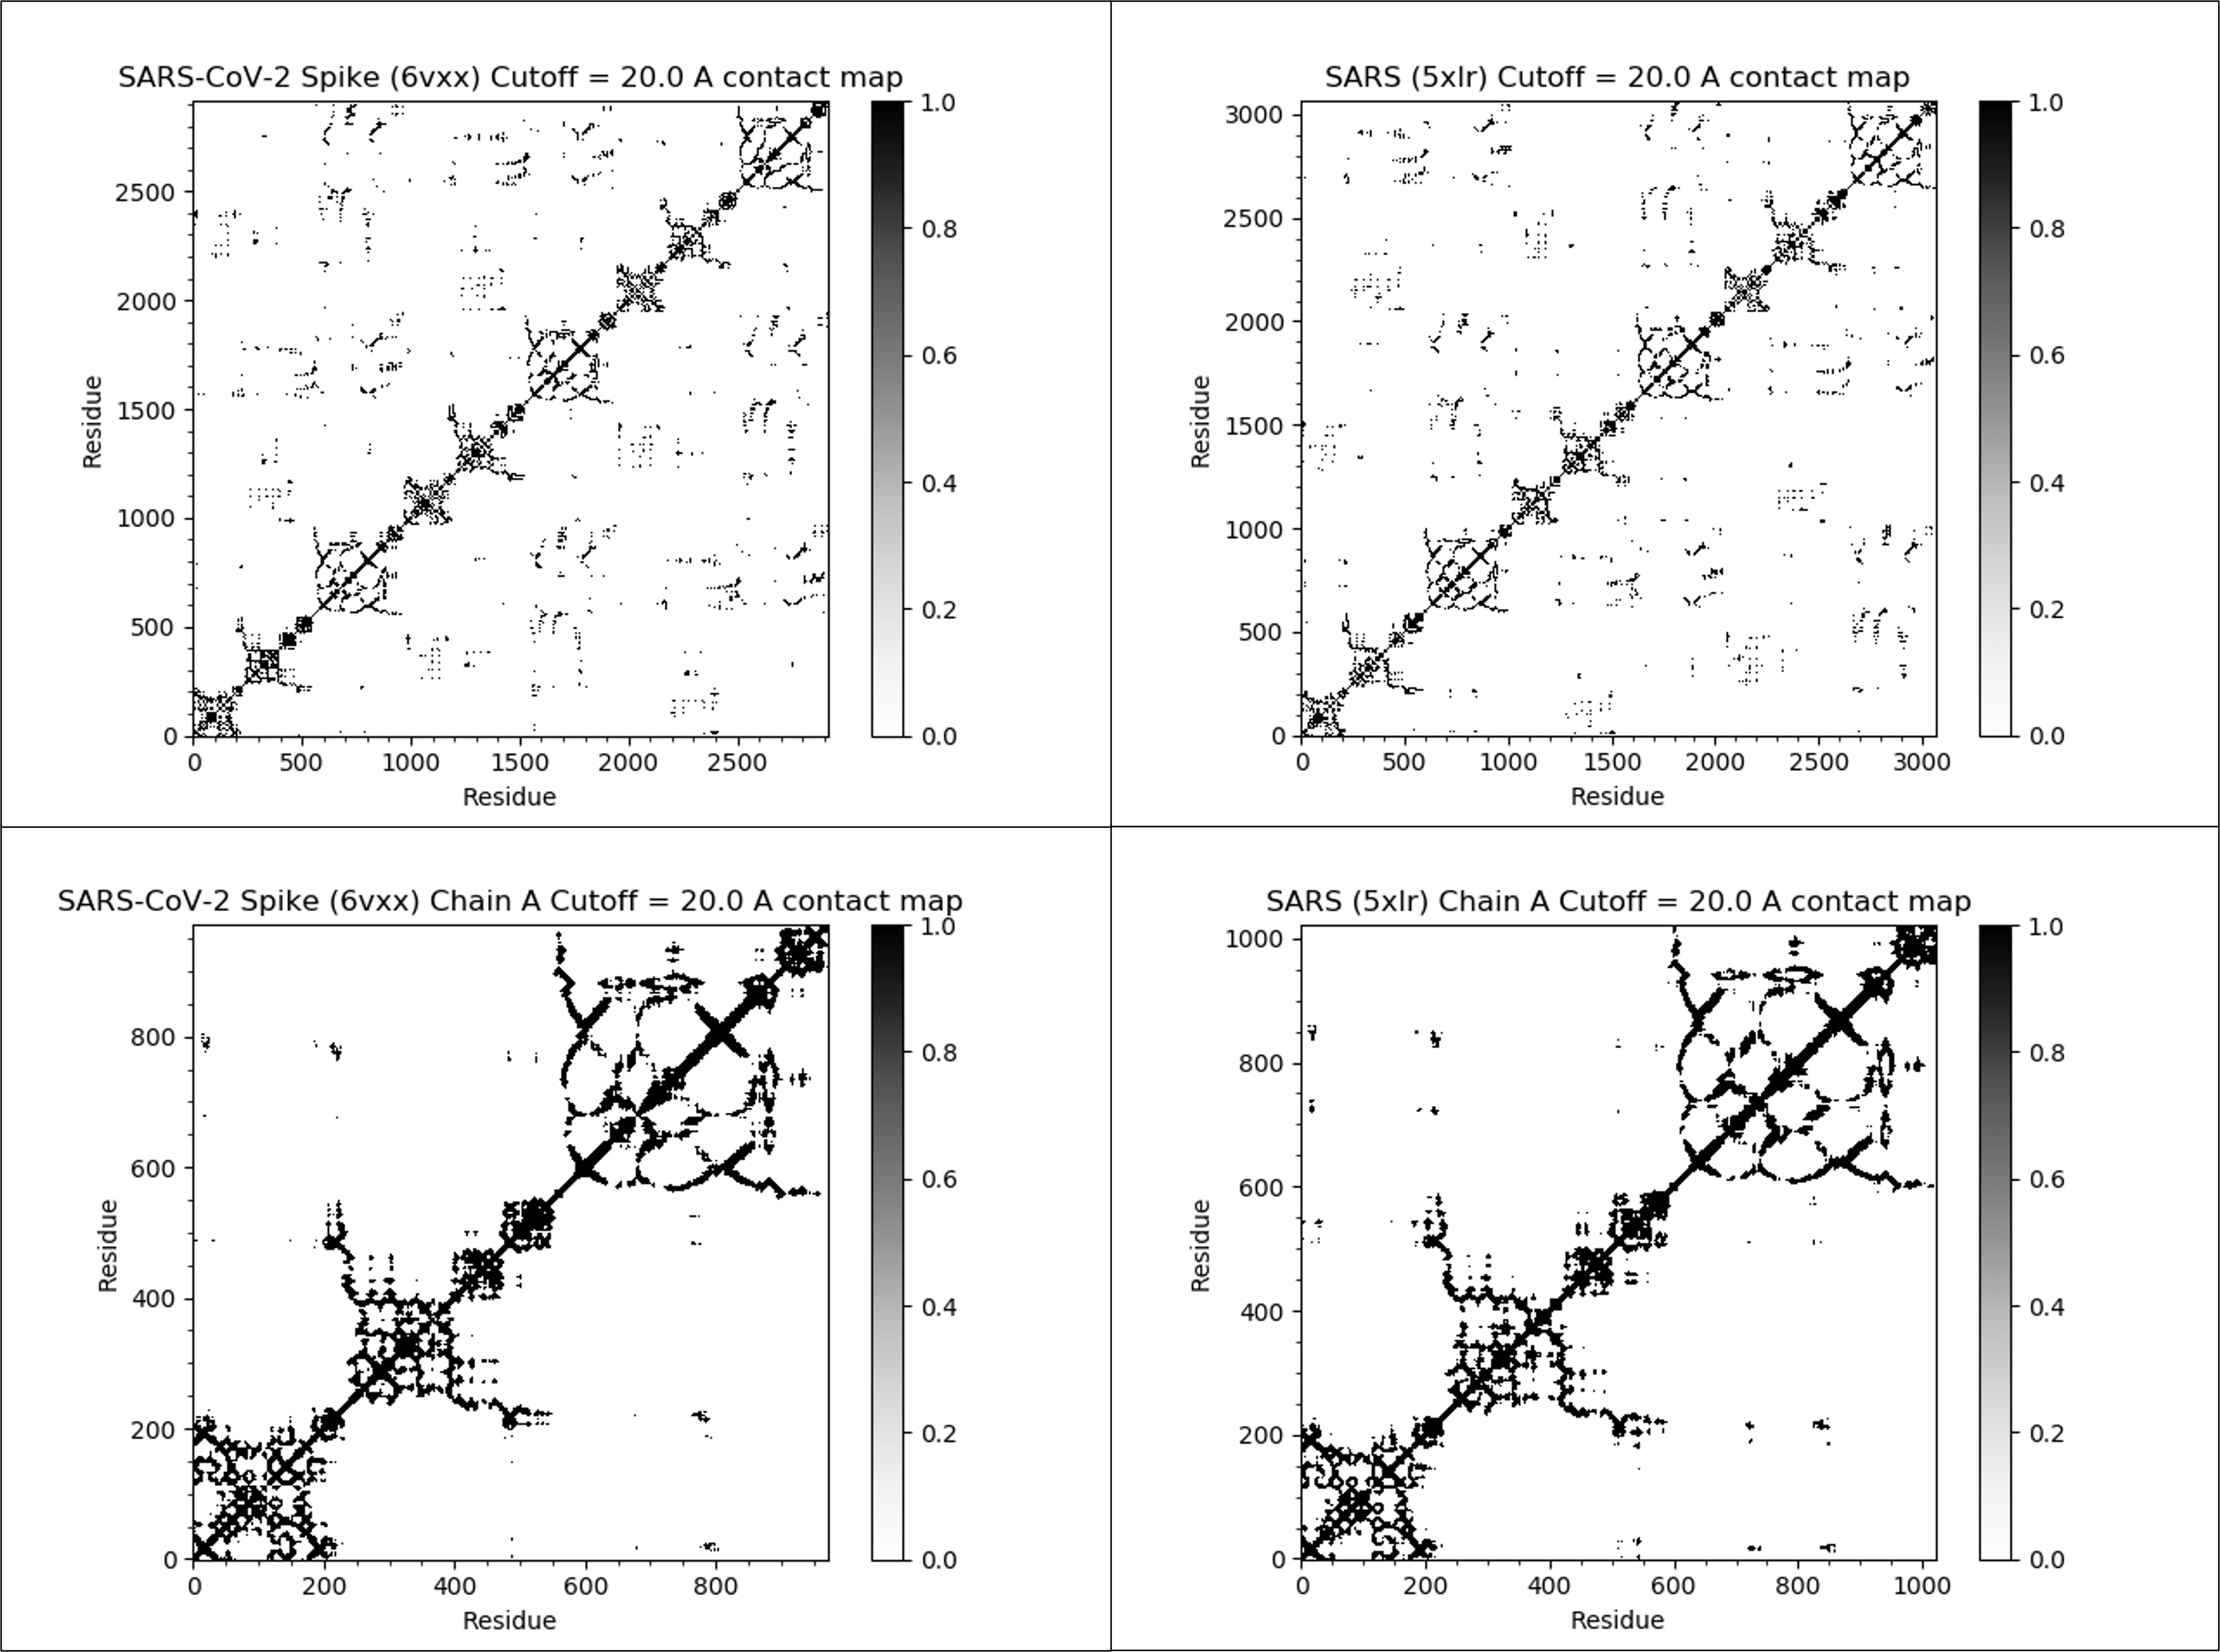
\includegraphics[width = 0.7\textwidth]{../images/Contact.png}
	\caption{The contact maps of the SARS-CoV-2 spike protein (top left), SARS-CoV spike protein (top right), single chain of the SARS-CoV-2 spike protein (bottom left), and single chain of the SARS-CoV spike protein (bottom right). If the distance between the \textit{i}-th and \textit{j}-th amino acids in a protein structure is 20.0 angstroms or less, then the (\textit{i}, \textit{j})-th cell of the figure is colored black. The SARS-CoV-2 and SARS spike proteins have very similar contact maps, indicating similar global structures.}
	\label{fig:Contact}
\end{figure}

\begin{qbox}[%
	How do you think the contact map will change as we increase or lower the threshold distance?
]\end{qbox}

We obtain some insight into how two proteins differ structurally at the $i$-th amino acid if we look at all of the $i$-th row's values; that is, if we compare all of the $d(s_{i}, s_{j})$ values to all of the $d(t_{i}, t_{j})$ values.

We will use pairwise distances between alpha carbons to determine how different two proteins are at the $i$-th alpha carbon, using a metric called \textdef{Q per residue (Qres)}{Q per residue (Qres)}{FILL IN}.  The formal definition of Qres for two structures $s$ and $t$ having $N$ residues is

$$Q_{\text{res}}^{(i)} = \dfrac{1}{N-k} \sum^{\text{residues}}_{j\neq i-1,i,i+1} \textrm{exp}[-\dfrac{[d(s_i,s_j)-d(t_i,t_j)]^2}{2\sigma^2_{i,j}}]\, .$$

In this equation, \testit{exp(x)} means $e^{x}$. This equation also includes the following parameters.

\begin{itemize}
	\item $k$ is equal to 2 at either the start or the end of the protein (i.e., $i$ is equal to 1 or $N$), and $k$ is equal to 3 otherwise.
	\item The variance term $\sigma_{ij}^2$ is equal to $\left\lvert{i-j}\right\rvert ^{0.15}$, which corresponds to the sequence separation between the $i$-th and $j$-th alpha carbons.
\end{itemize}

\begin{note}[%
	The above definition assumes that the two proteins have the same length or have been pre-processed by removing amino acids that only occur in one protein. Generalizations of Qres for proteins of non-equal length exist that first align proteins and retain only those amino acids for structural comparison that are shared by the two proteins.
]\end{note}

If two proteins are very similar at the $i$-th alpha carbon, then for every $j$, $d(s_{i}, s_{j}) - d(t_{i}, t_{j})$ will be close to zero, making term inside the summation in the Qres equation will be close to 1. The sum will be equal to approximately $N - k$, and so Qres will be close to 1. As two proteins become more different at the $i$-th alpha carbon, then the term inside the summation will head toward zero, and so will the Qres value as well.

As a result, we think of Qres as a similarity metric ranging between 0 and 1, with low scores representing low similarity between two proteins at the $i$-th position, and higher scores representing high similarity at this position.

We now will compute Qres for the SARS-CoV and SARS-CoV-2 spike proteins using the VMD plugin \textit{Multiseq} \url{https://www.ks.uiuc.edu/Research/vmd/plugins/multiseq/}, a bioinformatics analysis environment. After determining Qres, we will visualize the individual locations where the two RBD regions differ. \tutorial[https://biologicalmodeling.org/coronavirus/tutorial_multiseq]

\FloatBarrier
\phantomsection
\subsection{Local comparison of spike proteins leads us to a region of interest}

By computing Qres at every position of the two coronavirus RBD regions, we can form a "structural" alignment of the two regions, as shown in the figure below. Blue columns correspond to amino acids with high Qres (meaning high structural similarity), and red columns correspond to amino acids with low Qres (meaning low structural similarity).

If we zoom in on the region around position 150 of the alignment, we find a 13-column region of the alignment within the RBD region for which Qres values are significantly lower than they are elsewhere. This region corresponds to positions 476 to 485 in the SARS-CoV-2 spike protein and is shown in \autoref{fig:QresResult}.

\begin{figure}[h]
	\centering
	\tabcolsep = 1em
	\mySfFamily
	\begin{tabular}{c}
		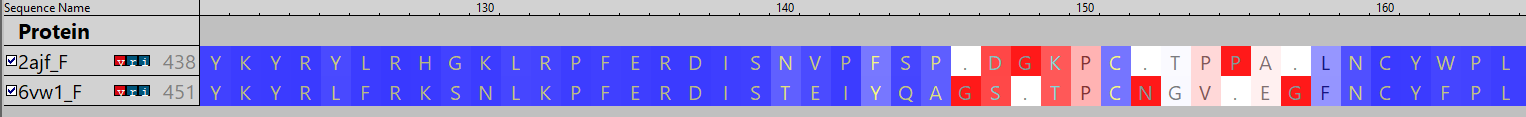
\includegraphics[width = 0.7\textwidth]{../images/QresResult.png} \\
		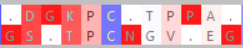
\includegraphics[width = 0.7\textwidth]{../images/QresResult_cropped.png} \\
	\end{tabular}
	\caption{(Top) A snapshot of the sequence alignment between the SARS-CoV RBD (first row) and the SARS-CoV-2 chimeric RBD (Shang et al. 2020) (second row). Columns are colored along a spectrum from blue (high Qres) to red (low Qres), with positions that correspond to an inserted or deleted amino acid colored red. (Bottom) A region of the alignment with low Qres, which corresponds to amino acids at positions 476 to 485 in the SARS-CoV-2 spike protein.}
	\label{fig:QresResult}
\end{figure}

We also can create a 3-D visualization of the structures. \autoref{QresVMD} shows the superimposed structures of both the SARS and SARS-CoV-2 RBD bound with ACE2, shown in green. The same color-coding of columns of the multiple alignment in the figure above is used to highlight differences between the SARS-CoV and SARS-CoV-2 structures. The low-Qres region of the RBM alignment that we highlighted in the above figure is outlined in \autoref{QresVMD}.

\begin{figure}[h]
	\centering
	\mySfFamily
	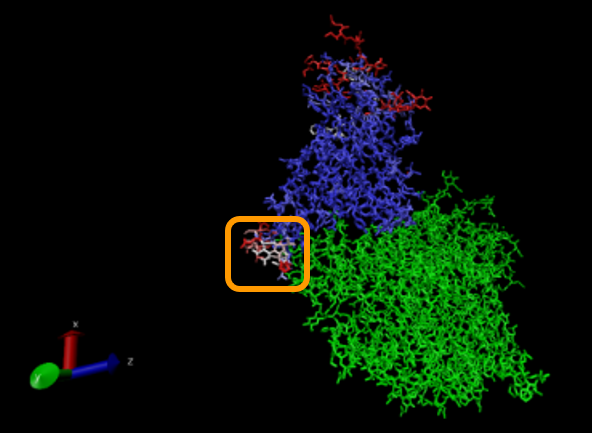
\includegraphics[width = 0.7\textwidth]{../images/QresVMD.png}
	\caption{A visualization showing the superposed structures of SARS-CoV-2 chimeric RBD (Shang et al. 2020) and SARS RBD in blue and red based on Qres. Blue indicates regions of high Qres, and red indicates regions of low Qres. ACE2 is shown in green. The highlighted region corresponds to the part of the RBM with a potential structural difference. Because it is adjacent to ACE2, it is likely that the structural difference here will affect ACE2 interactions.}
	\label{fig:QresVMD}
\end{figure}

\begin{note}[%
	Although the rest of the proteins are similar, there are other parts of the RBD at the top of the protein that show dissimilarities in the two proteins, which may be attributable to an experimental artifact. The authors of the work in which the comparison was published have pointed out that the highlighted region is unlikely to be an artifact of the experimentation because it is "buried at the RBD–ACE2 interface and did not affect crystallization".
]\end{note}

Finding this highlighted region in the RBM where the structures of the SARS-CoV and SARS-CoV-2 spike proteins differ is an exciting development. We will next explore this region of the protein structure to determine whether the mutations acquired by SARS-CoV-2 may have influenced the binding affinity of the virus spike protein with the human ACE2 enzyme.

\FloatBarrier
\phantomsection

\section{Analysis of Structural Protein Differences}
\label{sec:structural_differences}
\phantomsection
\subsection{Visualizing a region of structural differences}

In \autoref{sec:multiseq}, we identified a region between residues 476 and 485 of the SARS-CoV-2 spike protein that corresponds to a structural difference between the SARS-CoV-2 and SARS-CoV RBMs. We now wish to determine whether the differences we have found affect binding affinity with the human ACE2 enzyme.

We know from our work in this course that a tiny change can produce a big difference in the high-level behavior of a finely tuned system. It may therefore be the case that subtle changes in the ability of SARS-CoV-2 to stick to the ACE2 enzyme can change the virus's infectiousness enough to greatly influence its spread through the human population.

We will first use VMD to highlight the amino acids in the region of interest of the SARS-CoV-2 spike protein's structure. \tutorial[https://biologicalmodeling.org/coronavirus/tutorial_visualization]

\FloatBarrier
\phantomsection
\subsection{Analyzing three sites of conformational differences}

Shang et al. identified three sites showing significant conformational differences between the SARS-CoV-2 and SARS-CoV spike proteins. We will discuss each of these three locations and see how they affect binding affinity between the spike protein and ACE2.

\FloatBarrier
\phantomsection
\subsection{Site 1: loop in ACE2-binding ridge}

The first location is our region of interest from the previous section and is found on a loop in a region called the ACE2 binding ridge. This region is shown in the figure below, in which SARS-CoV-2 is on left and SARS-CoV is on the right.

Structural differences are challenging to show with a 2-D image,so we encourage you to use VMD to view the 3-D representation of the protein. \tutorial[https://biologicalmodeling.org/coronavirus/tutorial_multiseq]

\begin{qbox}[%
	See if you can identify the major structural difference between the proteins in \autoref{fig:Ridge}. Hint: look at the yellow residue.
]\end{qbox}

\begin{figure}[h]
	\centering
	\mySfFamily
	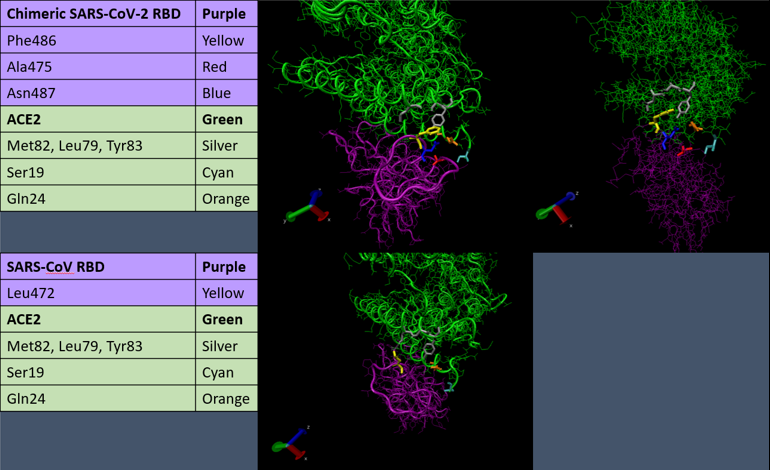
\includegraphics[width = 0.7\textwidth]{../images/Ridge.png}
	\caption{A visualization of the loop in the ACE2-binding ridge that is conformationally different between SARS-CoV-2 (left) and SARS-CoV (right). The coronavirus RBD is shown in purple, and ACE2 is shown in green. Structural differences cause certain amino acid residues (highlighted in various colors) to behave differently between the two interactions.}
	\label{fig:Ridge}
\end{figure}

The most noticeable difference between SARS-CoV-2 and SARS-CoV in this region relates to a "hydrophobic pocket" of three hydrophobic ACE2 residues at positions 82, 79, and 83 (methionine, leucine, and tyrosine). This pocket, which is colored silver in the above figure, is hidden away from the outside of the ACE2 enzyme to keep these amino acids away from water. In SARS-CoV-2, the RBD phenylalanine residue at position 486 (yellow) inserts itself into the pocket, favorably interacting with ACE2. These interactions do not happen with SARS-CoV, and its corresponding RBD residue, a leucine at position 472 (yellow), is not inserted into the pocket.

In what follows, we use a three-letter identifier for an amino acid followed by a number to indicate the identity of that amino acid followed by its position within the protein sequence. For example, the phenylalanine at position 486 of the SARS-CoV-2 spike protein would be called Phe486.

Although the interaction with the hydrophobic pocket is the most critical difference between SARS-CoV-2 and SARS-CoV, we highlight two other key differences. First, in SARS-CoV-2, a main-chain hydrogen bond forms between Asn487 and Ala475 (shown in red in \autoref{fig:Ridge}), which creates a more compact ridge conformation, pushing the loop containing Ala475 closer to ACE2. This repositioning allows for the N-terminal residue Ser19 of ACE2 (colored cyan in the above figure) to form a hydrogen bond with the main chain of Ala475. Second, Gln24 in ACE2 (colored orange in the above figure) forms a new contact with the RBM.

\FloatBarrier
\phantomsection
\subsection{Site 2: hotspot 31}

\textbf{Hotspot 31} is not a failed Los Angeles nightclub but rather our second region of notable conformational differences between SARS-CoV-2 and SARS-CoV, which was studied in SARS-CoV as early as 2008. This location earns its name because it involves a "salt bridge", or a combination of hydrogen and ionic bonding between two amino acids, that takes place between Lys31 and Glu35. Hotspot 31 is colored red in the figure below.

\begin{qbox}[%
	Once again, see if you can spot the differences between SARS-CoV-2 and SARS-CoV.
]\end{qbox}

\begin{figure}[h]
	\centering
	\mySfFamily
	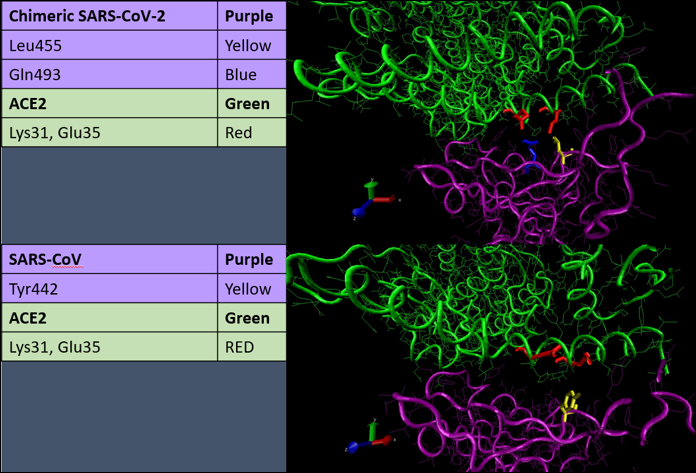
\includegraphics[width = 0.7\textwidth]{../images/Hotspot31.png}
	\caption{Visualizations of hotspot 31 in SARS-CoV-2 (left) and SARS-CoV (right). The RBD is shown in purple, and ACE2 is shown in green. In SARS-CoV, hotspot 31 corresponds to a salt bridge, which is broken in SARS-CoV-2 to form a new hydrogen bond.}
	\label{fig:Hotspot31}
\end{figure}

The figure above shows how the salt bridge is radically different in the two viruses. In SARS-CoV, the two residues appear to point towards each other because in the SARS-CoV RBM, Tyr442 (colored yellow in right figure) supports the salt bridge between Lys31 and Glu35 on ACE2. In contrast to Tyr442 in SARS-CoV, the corresponding amino acid in SARS-CoV-2 is the less bulky Leu455 (colored yellow in left figure), which provides less support to Lys31. This causes the salt bridge to break, so that Lys31 and Glu35 of ACE2 point in parallel toward the RBD residue Gln493 (colored blue). This change allows Lys31 and Glu35 to form hydrogen bonds with Gln493 in SARS-CoV-2.

\FloatBarrier
\phantomsection
\subsection{Site 3: hotspot 353}

Finally, we consider \textbf{hotspot 353}, which involves another salt bridge connecting Lys353 and Asp38 of ACE2. In this region, the difference between the residues is so subtle that it takes a keen eye to notice them in \autoref{fig:Hotspot353}.

\begin{figure}[h]
	\centering
	\mySfFamily
	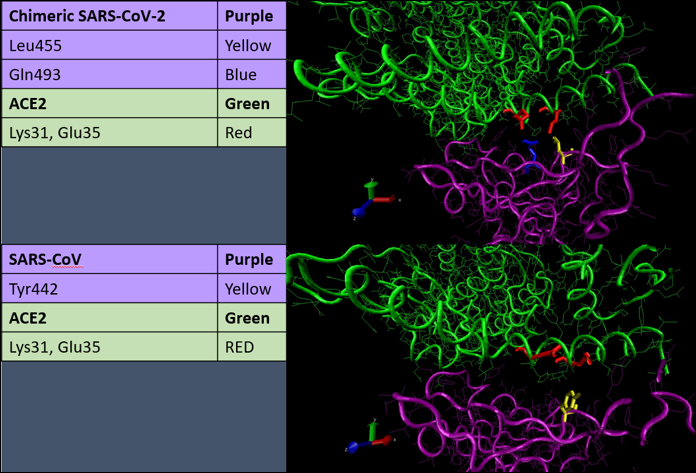
\includegraphics[width = 0.7\textwidth]{../images/Hotspot31.png}
	\caption{Visualizations of hotspot 353 in SARS-CoV-2 (left) and SARS-CoV (right). The RBD is shown in purple, and ACE2 is shown in green. In SARS-CoV, the RBD residue Thr487 (yellow) stabilizes the salt bridge between ACE2 residues Lys 353 and Asp38 (red). In SARS-CoV-2, the corresponding RBD residue Asn501 (yellow) provides less support, causing ACE2 residue Lys353 (red residue on the left) to be in a slightly different conformation and form a new hydrogen bond with the RBD.}
	\label{fig:Hotspot31}
\end{figure}

In SARS-CoV, the methyl group of Thr487 (colored yellow in the right figure above) supports the salt bridge on ACE2, and the side-chain hydroxyl group of Thr487 forms a hydrogen bond with the RBM backbone. The corresponding SARS-CoV-2 amino acid Asn501 (colored yellow in left figure) also forms a hydrogen bond with the RBM main chain. However, similar to what happened in hotspot 31, Asn501 provides less support to the salt bridge, causing Lys353 on ACE2 (colored red) to be in a different conformation. This allows Lys353 to form an extra hydrogen bond with the main chain of the SARS-CoV-2 RBM while maintaining the salt bridge with Asp38 on ACE2.

You may be wondering how researchers can be so fastidious that they would notice all these subtle differences between the proteins, even if they know where to look. The fact is that they have help in their subjective descriptions of how protein structure affects binding. In the next section, we will discuss how to \textit{quantify} the improved binding of SARS-CoV-2 to ACE2 at the three locations described above.

\FloatBarrier
\phantomsection

\section{Quantification of Protein Interaction Energy}
\label{sec:interaction_energy}
\phantomsection
\subsection{Computing energy of a bound complex}

In part 1 of this chapter, we searched for the tertiary structure that best "explains" a protein's primary structure by looking for the structure with the lowest potential energy (i.e., the one that is the most chemically stable).

To quantify whether two molecules bind well, we will borrow this idea and compute the potential energy of the complex formed by the viral spike protein and ACE2. If two molecules bind well, then the complex will have a very low potential energy. In turn, if we compare the SARS-CoV-2 RBD-ACE2 complex against the SARS-CoV RBD-ACE2 complex, and we find that the potential energy of the former is significantly smaller, then we can conclude that it is more stable, providing evidence for the increased infectiousness of SARS-CoV-2.

In the following tutorial, we will compute the energy of the bound spike protein-ACE2 complex for the two viruses and see how the three regions that we identified in \autoref{sec:structural_differences} contribute to the total energy of the complex. To do so, we will employ NAMD (\url{https://www.ks.uiuc.edu/Research/namd/}), a program that was designed for high-performance large system simulations of biological molecules and is most commonly used with VMD via a plugin called NAMD Energy (\url{https://www.ks.uiuc.edu/Research/vmd/plugins/namdenergy/}). This plugin will allow us to isolate a specific region to evaluate how much this local region contributes to the overall energy of the complex. \tutorial[https://biologicalmodeling.org/coronavirus/tutorial_NAMD]

\FloatBarrier
\phantomsection
\subsection{Differences in interaction energy with ACE2 between SARS and SARS-CoV-2}

\autoref{fig:NAMDEnergy2} shows the interaction energies for each of our three regions of interest as well as the total energy of the complex with ACE2 for both SARS-CoV and SARS-CoV-2.

\begin{figure}[h]
	\centering
	\mySfFamily
	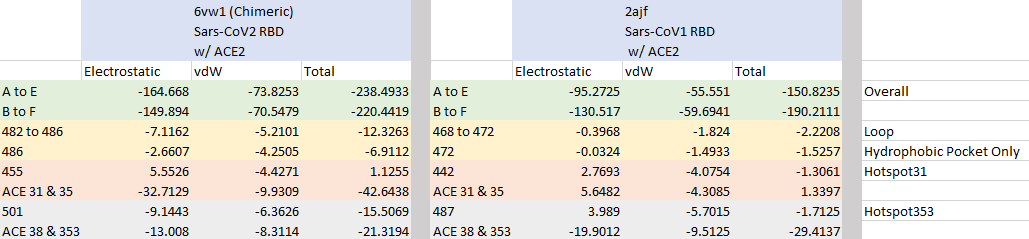
\includegraphics[width = 0.7\textwidth]{../images/NAMDEnergy2.png}
	\caption{ACE2 interaction energies of the chimeric SARS-CoV-2 RBD and SARS RBD. The PDB files contain two biological assemblies, or instances, of the corresponding structure. The first instance includes chain A (ACE2) and chain E (RBD), and the second instance includes chain B (ACE2) and chain F (RBD). The overall interactive energies between the RBD and ACE2 are shown in the first two rows (green). Then, the individual interaction energies are shown from the loop site (yellow), hotspot 31 (red), and hotspot 353 (grey). Total energy is computed as the sum of electrostatic interactions and van der Waals (vdW) forces.}
	\label{fig:NAMDEnergy2}
\end{figure}

We can see in the table that the overall attractive interaction energy between the RBD and ACE2 is lower for SARS-CoV-2 than for SARS-CoV, which supports previous studies that have found the SARS-CoV-2 spike protein to have higher affinity with ACE2.

Furthermore, all of the three regions of interest have a lower total energy in SARS-CoV-2 than in SARS-CoV, with hotspot 31 (red) having the greatest negative contribution. We now have quantitative evidence that the conformational changes in the three sites do indeed increase the binding affinity between the spike protein and ACE2.

Nevertheless, we should be careful with making inferences about the infectiousness of SARS-CoV-2 based on these results. To add evidence for our case, we would need biologists to perform additional experimental work to demonstrate that the improved binding of SARS-CoV-2 translates into greater infectiousness in human cells.

Another reason for our cautiousness is that proteins are not fixed objects but rather \textit{dynamic} structures whose shape is subject to small changes over time. In the conclusion to part 2 of this chapter, we will learn how to analyze the dynamics of a protein's movements within its environment.